%***********************************************************************
%* File            :    MAIN.tex
%*
%* HAUPTDOKUMENT
%*
%* Dieses Dokument bindet alle untergeordneten Dokumente
%* ein. Es wird beim Aufruf von pdflatex als Quelle angegeben.
%*
%* Autoren         :    Daniel Hering, Tobias Wartzek
%*
%* Datum           :    05.12.2009
%***********************************************************************



\documentclass[12pt,a4paper,twoside,openright,index=totoc,listof=totoc,BCOR=8.25mm,headinclude,footinclude=false,headsepline,notitlepage,numbers=noenddot,bibliography=totoc,headings=normal,parskip=full]{scrbook}

%************************************************************************
% Das Package muss leider hier eingebunden werden da sonst in den
% Befehlen f�r hypersetup keinerlei Umlaute zur Verf�gung stehen
%************************************************************************

\usepackage[latin1]{inputenc}            % erlaubt direkte Eingabe Deutscher
                                         % Sonderzeichen in .tex Dateien
                                         %(latin1=iso8859-1 fuer Unix Editoren
                                         % oder Windows Editoren die auch latin1
                                         % beherrschen)

%\usepackage[ngerman, english]{babel}
\usepackage[english]{babel}
\usepackage{tabularx}
\usepackage{multirow}
\usepackage{graphicx}
\usepackage{subfig}
\usepackage{booktabs}
%************************************************************************
% Dateiinfos eintragen (u.a. von hypersetup und f�r die Titelseite verwendet)
%************************************************************************
\usepackage{pdfpages}
% Titel der Arbeit
\newcommand*{\doclongtitle}{Modeling and flow control for a left ventricular assist device}

% Art der Arbeit (Diplomarbeit, Studienarbeit, Bachelorarbeit, etc.)
\newcommand*{\docsubject}{Master Thesis}

% Name des Autors
\newcommand*{\docauthor}{Julia Ribbrock}

% E-Mail Adresse des Autors
\newcommand*{\docauthoremail}{julia.ribbrock@rwth-aachen.de}

% Schl�sselworte der Arbeit
\newcommand*{\dockeywords}{MedIT Latex Studienarbeit Diplomarbeit Vorlage}

% Name des Betreuers
\newcommand*{\docsupervisor}{Patrick Borchers, M.Sc.}

\newcommand*{\docauthorfax}{+49 241 80-6-23211}
\newcommand*{\docauthorphone}{+49 241 80-23211}

% Bild auf der Titelseite
\newcommand*{\doctitlepic}{images/beispiel1}

% folgende Befehle nicht �ndern!!
\newcommand*{\dochomepage}{www.medit.hia.rwth-aachen.de}
\newcommand*{\docshorttitle}{\doclongtitle}

%**********************************************
%* Pakete (HEADER)                           *
%**********************************************

\include{HEADER}


%*************************************************************
%*************************************************************
%*																													**
%* 					Beginn des Dokuments 						  							**
%*																													**
%*************************************************************
%*************************************************************

\begin{document}
\begin{sloppypar}                       % sch�ner Blocksatz trotz langer Worte



%*************************************************************
%																														 *
%										 ENDE ALLER DEFINITIONEN 								 *
%																														 *
%*************************************************************


\frontmatter    												%r�mische Nummerierung aktivieren
%***********************************************************************
%* File            :    titel2.tex
%*
%* Titelseite
%*
%* Autor           :    Daniel Hering
%***********************************************************************

\newcommand{\defaultarraystretch}{\arraystretch}

\begin{titlepage}
\enlargethispage{31mm}
%***********************************************************************
%* Definition der Kopfzeile																						 *
%***********************************************************************
\vspace*{-3cm}
\hspace*{-1.8em}
\begin{tabularx}{19cm}{Xl@{}}
\textsf{\textbf{\LARGE{\docsubject}}} & %\includegraphics[height=45pt]{images/RWTH_Aachen_University}
\\
\mbox{\vspace{-10mm}\colorbox{rwthblue}{\hspace{18.4cm}}
\rule{0pt}{10pt}}
%\vspace{-10mm}\colorbox{rwthblue}{\hspace{12.7cm}}  {\includegraphics[height=30pt]{images/medit_l_m_blau_meditheadfoot}}
\end{tabularx}

%***********************************************************************
%* Ende der Definition der Kopfzeile																	 *
%***********************************************************************
\vspace*{15mm}
\par
\begingroup
\huge
\leftskip20pt
\noindent \textsf{\LARGE\docauthor\\
\textbf{\huge \docshorttitle}}
\par
\endgroup
\vfill % F�llt die Seite vertikal auf

%***********************************************************************
%* Hier eine zur Diplomarbeit geh�rende Grafik einbinden 							 *
%***********************************************************************
%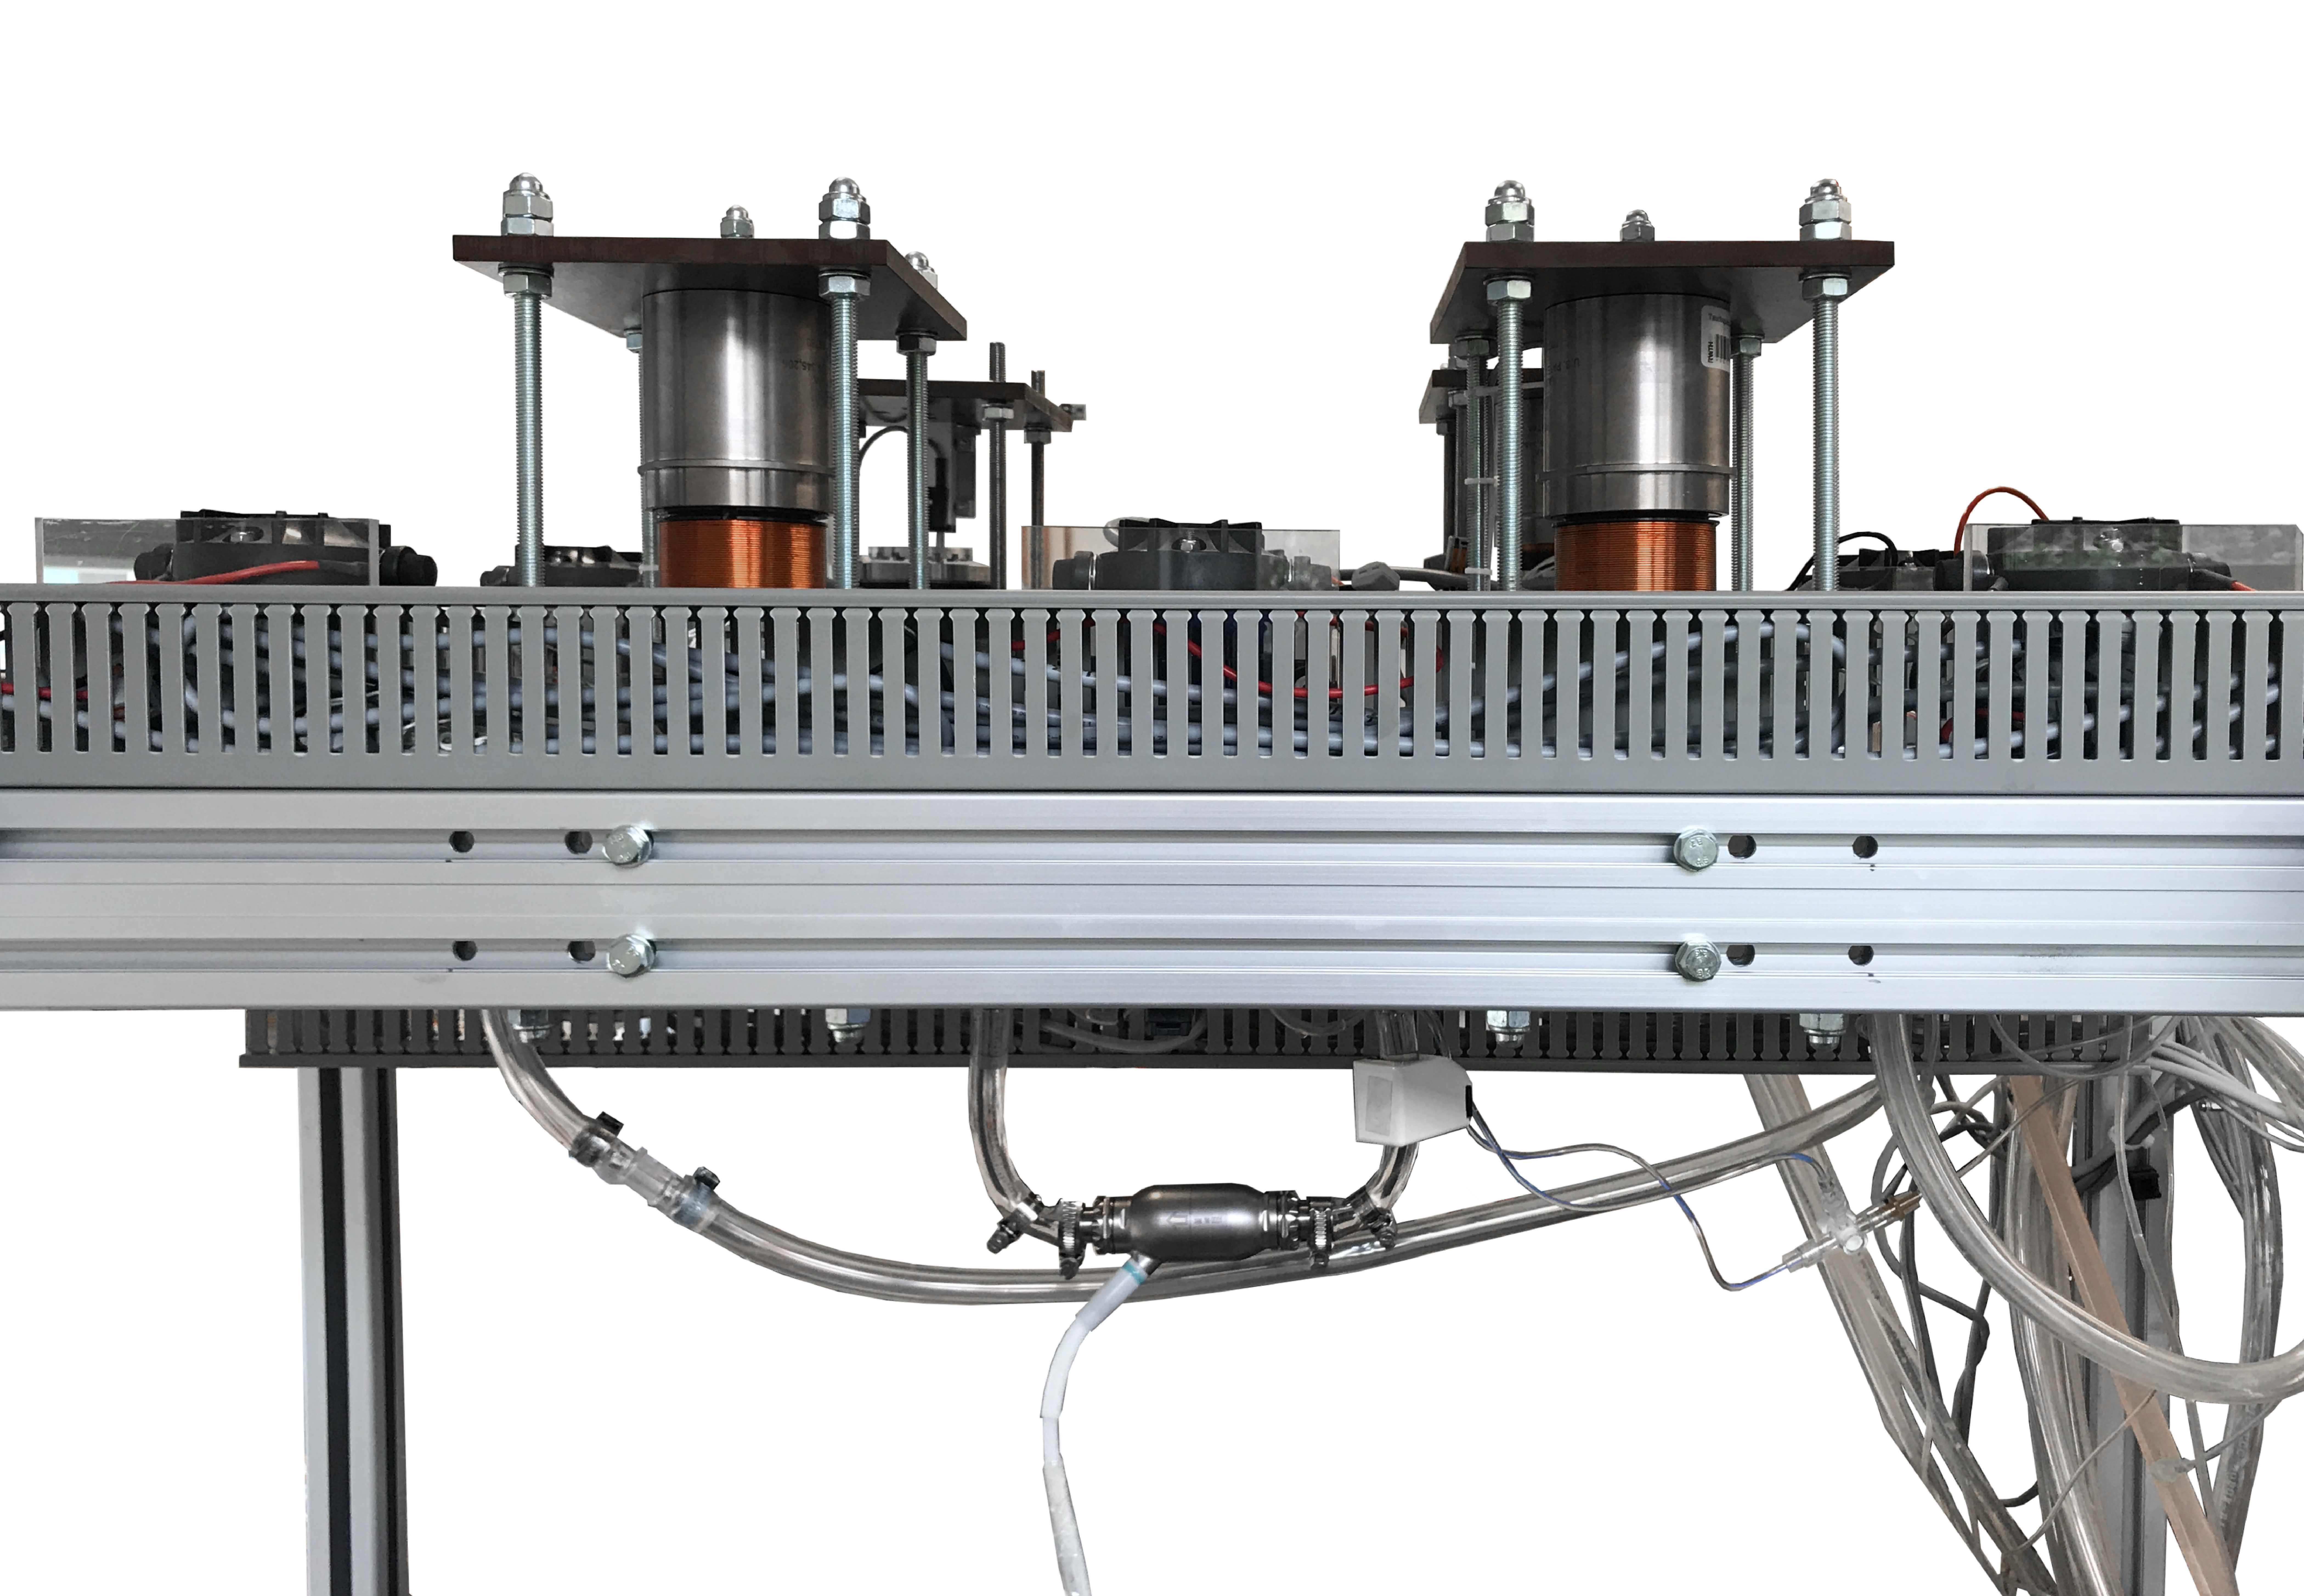
\includegraphics[width=0.9\textwidth]{images/Teststand_I.pdf}\vspace{10pt}

\AddToShipoutPicture*{
     \parbox[b][\paperheight]{\paperwidth}{%
       \vfill
        \centering
        \begin{tikzpicture}[overlay]%
       		  %\draw[help lines] (0,0) grid (10,20);
            \node (0,0) [opacity=0.8]{%
             \hspace{-8,25mm}\includegraphics[width=12cm, height=12cm,keepaspectratio]{\doctitlepic}};%
         \end{tikzpicture}
       \vspace{32.35em}
     }}







\renewcommand{\arraystretch}{1.3}
\hspace*{-1.8em}
\begin{tabularx}{19cm}{Xl}
\multicolumn{2}{l}{\colorbox{rwthblue}{\hspace{18.4cm}}}\\
\multicolumn{2}{l}{\textsf{\textbf{CHAIR FOR MEDICAL INFORMATION TECHNOLOGY}}}\\
\multicolumn{2}{l}{\textsf{{Faculty of Electrical Engineering and Information Technology, RWTH Aachen}}}\\
\multicolumn{2}{l}{\textsf{Univ.-Prof. Dr.-Ing. Dr. med. Dr. h.c. Steffen Leonhardt}}\\
\textsf{Supervisor: \docsupervisor} & \\
\textsf{Date: \today} & \multirow{-2}*~%{\includegraphics[height=30pt]{images/medit_l_m_blau_meditheadfoot}} \\
\end{tabularx}%}
\renewcommand{\arraystretch}{\defaultarraystretch}

\thispagestyle{empty}
\cleardoublepage

\end{titlepage}

%%***********************************************************************
%* File            :    titel.tex
%*
%* Titelseite 		 
%*
%* Autor           :    Daniel Hering
%***********************************************************************



\let\savedbaselinestretch=\baselinestretch    % Probleme mit geandertem 
                                              % baselinestretch umgehen
\renewcommand{\baselinestretch}{1}%
\begin{titlepage}

%***********************************************************************
%* Definition der Kopfzeile																						 *
%***********************************************************************

\titlehead{\vspace*{-15mm}\underline{\parbox[b]{\textwidth}{\includegraphics[height=24pt]{images/rwth_logo_blau_rechts}\parbox[b]{0.632\textwidth}{\raggedleft\textcolor{rwthblue}{\footnotesize{HELMHOLTZ-INSTITUT F�R BIOMEDIZINISCHE TECHNIK\\DER RWTH AACHEN}}}\includegraphics[height=24pt]{images/hia_logo_blau}}}\\\underline{\parbox[b]{\textwidth}{LEHRSTUHL F�R MEDIZINISCHE INFORMATIONSTECHNIK\\Univ.-Prof. Dr.-Ing. Dr. med. Steffen Leonhardt}}}

%***********************************************************************
%* Ende der Definition der Kopfzeile																	 *
%***********************************************************************

\subject{\vspace*{2\baselineskip}}
\title{\docshorttitle}
\author{
  \parbox{.8\linewidth}{%
     \centering\docauthor\\%
\vspace{0.7em}
\large Betreuer/-in: \docsupervisor\\
 \date{\large \today}
}
}%

\publishers{\small\vspace*{\stretch{1000}}%
  \parbox{\linewidth}{%
  \vspace{10cm}
    Pauwelsstra�e 20\\%
    D-52074 Aachen\\%
    Telefon: +49 (0)241 80 -23211\\%
    Fax: +49 (0)241 80 -82442\\%
    E-Mail: medit@hia.rwth-aachen.de\\%
  }%
  \vspace*{-\stretch{1}}%
}
\maketitle
\thispagestyle{empty}
\cleardoublepage
\let\baselinestretch=\savedbaselinestretch%
\end{titlepage}



\cleardoubleemptypage


%**************
%* Danksagung *
%**************

% \chapter{Acknowledgement}
% \thispagestyle{empty}
% As getting to the point of writing this thesis would not have been possible without the great help of some people, i would like to use this as an opportunity to say thanks.
%
% A big thank you goes out to my supervisor, Patrick Borchers (M.Sc.), who has always been at my side with kind words and information, pushing me through the finish line of this thesis.
%
% Furthermore i would like to thank Prof. Dr.-Ing. Dr. Med. Leonhardt, chairman of the chair for medical information technology, for enabling me to write this thesis.
%
% Last but not least, i want to thank all the wonderful people in my daily life, who all stood beside me during these challenging times of my studies, never doubting me especially when i've lost faith in this process.

\cleardoubleemptypage

%************************************************
%* Erkl�rung (hier muss nichts ge�ndert werden) *
%************************************************

\include{erklaerung}
\cleardoubleemptypage

%************
%* Abstract *
%************

\chapter{Abstract}

% Acute heart failure is one of the most common reasons for hospitalization due to heart diseases. As patients lifes at the final stages of heart failure depend on receiving a suitable donor heart and the numbers of cases does by far exceed the number of available donor organs, acute heart failure often results in patients death. Left ventricular assist devices (LVADs) have become a common treatment option in patients with heart insufficiency. They provide the ability to assist the patients heart in it's functionality of pumping blood through the circulatory system and thus can prolong a patients time span for proper treatment with a donor heart.
% \\
% The Sputnik VAD is a rotary blood pump that was recently developed by our project partner in Russia. In the course of this work,  first a model representation for the Sputnik LVAD will be developed and the parameters of this model will be identified. The model will then be used to design a current and a speed control. Furthermore, a cascaded flow control is to be designed in order to be able to specify arbitrary flow trajectories. Additionally, different Iterative Learning Controls will be implemented and compared. The control algorithms will be implemented using Matlab and Simulink. Finally, the different control approaches will be evaluated on a cardiovascular simulator developed at MedIT.


% VAD6 for abstract/introduction input

\cleardoubleemptypage
\thispagestyle{empty}

\cleardoubleemptypage

%**********************
%* Inhaltsverzeichnis *
%**********************


\addcontentsline{toc}{chapter}{Contents} % Eintrag im Inhaltsverzeichnis erstellen
\tableofcontents                        % Inhaltsverzeichnis anlegen√
\cleardoubleemptypage

%\addcontentsline{toc}{chapter}{List of Figures}
\listoffigures
\cleardoubleemptypage

\listoftables
\cleardoubleemptypage


%*********************
%* Symbolverzeichnis *
%********************

\chapter*{List of Symbols}										% da *-Variante m�ssen Kopfzeilen und TOC-Eintrag von Hand generiert werden
\markboth{List of Symbols}{List of Symbols} 				% Kopfzeile manuell anpassen
\addcontentsline{toc}{chapter}{List of Symbols}				% TOC-Eintrag



\section*{Abbreviations}
%
\acrodef{AV}[AV]{Atrioventricular}
\acrodef{bpm}[bpm]{beats per minute}
\acrodef{BTD}[BTD]{Bridging to decision}
\acrodef{BTR}[BTR]{Bridging to recovery}
\acrodef{BTT}[BTT]{Bridging to transplantation}
\acrodef{BVAD}[BVAD]{Biventricular Assist Device}
\acrodef{CHR}[CHR]{Chien Hrones Reswick}
\acrodef{CO}[CO]{Cardiac Output}
\acrodef{CVDs}[CVDs]{Cardiovascular Diseases}
\acrodef{CVS}[CVS]{Cardiovascular System}
\acrodef{DT}[DT]{Destination therapy}
\acrodef{EDV}[EDV]{End-diastolic volume}
\acrodef{EF}[EF]{Ejection fraction}
\acrodef{ESV}[ESV]{End-systolic volume}
\acrodef{ILC}[ILC]{Iterative learning control}
\acrodef{IMACS}[IMACS]{International Mechanically Assisted Circulatory Support}
\acrodef{INTERMACS}[INTERMACS]{Interagency Registry for Mechanically Assisted Circulatory Support}
\acrodef{HiL}[HiL]{Hardware in the Loop}
\acrodef{HR}[HR]{Heart rate}
\acrodef{HTx}[HTx]{Heart transplantation}
\acrodef{LVAD}[LVAD]{Left Ventricular Assist Device}
\acrodef{MCL}[MCL]{Mock circulatory loop}
\acrodef{MCS}[MCS]{Mechanical Circulatory Support}
\acrodef{MISO}[MISO]{Multiple-input-single-output}
\acrodef{RMSE}[RMSE]{Root Mean Square Error}
\acrodef{RWTH}[RWTH]{Rheinisch-Westf{\"a}lische Technische Hochschule}
\acrodef{RVAD}[RVAD]{Right Ventricular Assist Device}
\acrodef{SISO}[SISO]{Single-input-single-output}
\acrodef{SL}[SL]{Semilunar}
\acrodef{SV}[SV]{Stroke Volume}
\acrodef{VADs}[VADs]{Ventricular Assist Devices}
\acrodef{WHO}[WHO]{World Health Organization}
\acrodef{ZN}[ZN]{Ziegler Nichols}

%* \acs{Name} ruft explizit die Abk�rzung auf.
%* \acl{Name} ruft explizit den ausgeschriebenen Begriff auf.

\begin{tabbing}
  ---------------------\=--------------------------------\kill
%\begin{tabularx}{\textwidth}{p{.18\textwidth}X}
  \textbf{A}\\
\acs{AV}       \> \acl{AV} \\
\\
\textbf{B}\\
\acs{bpm}       \> \acl{bpm} \\
\acs{BTD}       \> \acl{BTD} \\
\acs{BTR}       \> \acl{BTR} \\
\acs{BTT}       \> \acl{BTT} \\
\acs{BVAD}       \> \acl{BVAD} \\
\\
\textbf{C}\\
\acs{CHR}       \> \acl{CHR} \\
\acs{CO}       \> \acl{CO} \\
\acs{CVDs}       \> \acl{CVDs} \\
\acs{CVS}       \> \acl{CVS} \\
\\
\textbf{D}\\
\acs{DT}       \> \acl{DT} \\
\\
\textbf{E}\\
\acs{EDV}       \> \acl{EDV} \\
\acs{EF}       \> \acl{EF} \\
\acs{ESV}       \> \acl{ESV} \\
\\
\textbf{H}\\
\acs{HiL}       \> \acl{HiL} \\
\acs{HR}       \> \acl{HR} \\
\acs{HTx}       \> \acl{HTx} \\
\\
\\
\pagebreak
\textbf{I}\\
\acs{ILC}       \> \acl{ILC} \\
\acs{IMACS}       \> \acl{IMACS}\\
\acs{INTERMACS}       \> \acl{INTERMACS}\\
\\
\textbf{L}\\
\acs{LVAD}       \> \acl{LVAD} \\
\\
\textbf{M}\\
\acs{MCL}       \> \acl{MCL} \\
\acs{MCS}       \> \acl{MCS} \\
\acs{MISO}       \> \acl{MISO}\\
\\
\textbf{R}\\
\acs{RMSE}       \> \acl{RMSE}\\
\acs{RWTH}       \> \acl{RWTH}\\
\\
\textbf{S}\\
\acs{SISO}       \> \acl{SISO}\\
\acs{SL}       \> \acl{SL}\\
\acs{SV}       \> \acl{SV} \\
\\
\textbf{V}\\
\acs{VADs}       \> \acl{VADs} \\
\\
\textbf{W}\\
\acs{WHO}       \> \acl{WHO} \\
\\
\textbf{Z}\\
\acs{ZN}       \> \acl{ZN} \\
\end{tabbing}
%\end{tabularx}
%
% \section*{Physical parameters}
% \begin{tabbing}
%   ---------------------\=---------------------\=---------------------\kill
%   f \> frequency \> Hz\\
%   p \> pressure \> mmHg\\
%   q \> flow \> $\mathrm{l\min}$\\
%   t \> time \> s \\
%   T \> timespan \> s\\
%   v \> rotational speed \> rpm\\
%
% \end{tabbing}
%
% \section*{Mathematische Gr��en}
%
% \begin{tabularx}{\textwidth}{p{.18\textwidth}X}
% $\mathrm{M}$ & mathematische Beispielgr��e \\
% \end{tabularx}
%
% \section*{Indizes}
%
% \begin{tabularx}{\textwidth}{p{.18\textwidth}X}
% $k$ & Anzahl der Proze�schritte \\
% $P_{1}...P_{n}$ & Proze�schritt $P_{1}$ bis $P_{n}$\\
% $V_{Ziel}$ &  Zielvektor\\
% \end{tabularx}
%

\cleardoubleemptypage

\mainmatter							% Arabische Nummerierung, Beginn des Hauptteils

%**************
%* Einleitung *
%**************

\chapter{Introduction}
\section{Motivation and goal}

\section{Thesis structure}


%*************
%* Hauptteil *
%*************

\chapter{Medical Fundamentals}
Comprehension of the physiological functionality of the human heart and the cardiovascular system is an important prerequisite to the work addressed in this thesis. Therefore the basics of these topics will be explained in this chapter. 

\section{Anatomy of the Heart}

\section{Cardiovascular System}

\section{Heartinsufficency}

% \chapter{Technical Fundamentals}
% Since the main part of this thesis addresses the implementation of flow control algorithms for a left ventricular assist device, the basics of control theory and a introduction on iterative learning control will be presented here as well.

\chapter{Control Theory}
Since the field of control theory is very extensive, this section will only deal with the notation and structure of a standard control loop in general. Furthermore, the basic principles of a PI controller and an iterative learning control are discussed, since these are used within pratical part of the thesis.
\section{Fundamentals}
The basic task of control engineering is to influence a time-varying process from the outside with the goal that the process is executed in a predetermined manner. A control system is characterized in particular by the feedback of the controlled variable to the reference variable. The reference variable represents the state to be achieved.
In theory, this is represented by a control loop with the components shown in \figurename~{\ref{fig:control_loop}}.
\begin{figure}
  \centering
  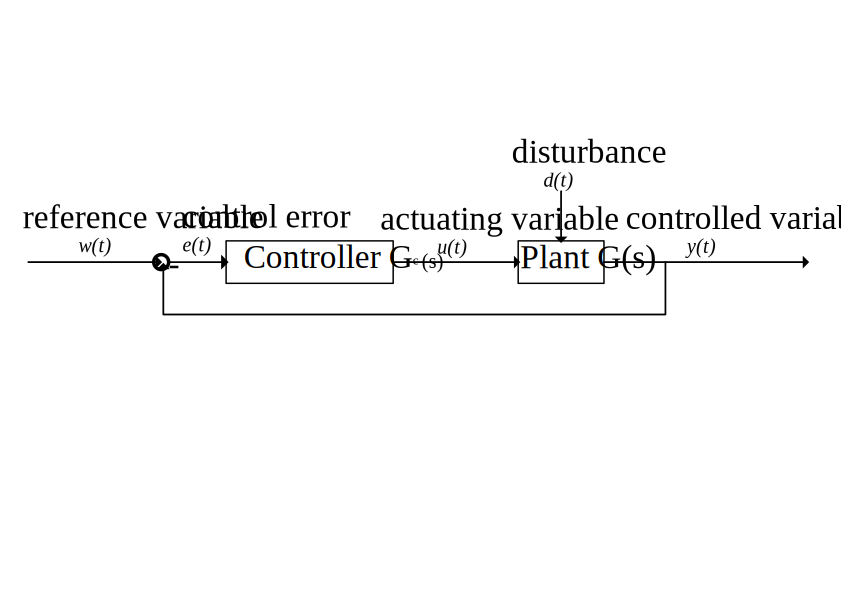
\includegraphics[width=0.9\textwidth]{images/control_loop.jpg}
  \caption[General structure of a control loop]{General structure of a control loop}
  \label{fig:control_loop}
\end{figure}
The plant $G(s)$ transfers the actuating variable $u(t)$, as well as the influence of the the disturbance $d(t)$, to the controlled variable $y(t)$. This variable is permanently compared with the reference variable $w(t)$ by means of a feedback. Which results in the control error
\begin{equation}
  e(t) = w(t) - y(t)
 \label{eq:e_t}
\end{equation}
The controller $G_{c}(s)$ then transfers the control error to the actuating variable again. The aim of the control loop is to achieve the smallest possible control error with the greatest possible damping. Since these goals contradict each other, a trade off must always be accepted here.\cite{Reg_17}
\\However, there are some general requirements for the closed control loop, which have to be fulfilled. The first of which states that the closed loop needs to be stable. This is the case when the control loop responds to a finite excitation with a finite output signal. The second one is the requirement for disturbance rejection, stating that the controlled variable needs to follow the reference variable asymptotically, so that
\begin{equation}
    \lim\limits_{t \rightarrow \infty}{e(t)} = 0
 \label{eq:lim_e}
\end{equation}
Another requirement is that the dynamic relationship between the reference variable w(t) and the controlled variable y(t) must satisfy specified quality requirements.  The last requirement states that the first three requirements must be statisfied despite uncertainties in the plant. This requirement is called the Robustness requirement. More detailed information on these requirements can be found in \cite{Reg_10}.

The plant $G(s)$ corresponds to the part of the system in which the physical quantity to be controlled is influenced by the controller. The calculation of the plant by setting up and solving differential equations is only possible in a few cases. Due to this, the determination of the plant's characteristic values is usually carried out experimentally. There are several basic types of plants. These are classified according to their dynamic behavior. As only the PT$_{1}$-element is used in the practical part of this thesis, all other variations will not be discussed at this point. Detailed information on this topic can be found in \cite{Reg_10}.
\\The PT$_{1}$-element is the plant type which is most common in technical equipment. A PT$_{n}$-element, in it's static state, reacts proportionally to the input value and has a distinct transition behavior. The index n describes the system order. A PT$_{1}$-element therefore is a proportional delay element of first order. The mathematical formulation of the transfer function of a PT$_{1}$-element is
\begin{equation}
    G(s) = \frac{k_{s}}{1+sT}
 \label{eq:tf_pt1}
\end{equation}

\begin{figure}[h]
   \centering
   \includegraphics[width=0.9\textwidth]{images/tf_pt1.jpg}
   \caption[Tranfer function of a PT$_{1}$-element]{Transfer function of a PT$_{1}$-element \cite{Reg_10}.}
   \label{fig:tf_pt1}
 \end{figure}
The value $k_{s}$ describes the static gain, which equals the final value of the transfer function, in case $u(0)=0$. The time constant T enables an impression of the speed with which the system can react to changes at the input. It is defined as the time at which the transfer function reaches 63\% of the static gain. \cite{Reg_10}
\figurename~\ref{fig:tf_pt1} shows the tranfer function of a PT$_{1}$-element.


\section{PI-controller}
A PI-controller is a control structure commonly used for linear systems. This structure consists of both a propotional and an integral control element.
The output value of a P-controller is proportional to it's input value. In relation to the control loop in \figurename~\ref{fig:control_loop} this leads to
\begin{equation}
    u(t) = K_{P}e(t).
 \label{eq:p_contr_1}
\end{equation}
Using Laplacetransformation the transfer function for a P controller can be determined as
\begin{equation}
    G(s) = \frac{u(s)}{e(s)} = K_{P}
 \label{eq:p_contr_2}
\end{equation}
Therefore, the step response of this controller equals a step weighted with the Parameter $K_{P}$.
The relationship between input and output value of an I-controller is described through
\begin{equation}
    u(t) = K_{I}\int e(t) dt.
 \label{eq:i_contr_1}
\end{equation}
Equal to the P-controller, Laplacetransformation can be used to determine the transfer function of the I-controller.
This leads to
\begin{equation}
    G(s) = \frac{u(s)}{e(s)} = \frac{K_{I}}{s},
 \label{eq:i_contr_2}
\end{equation}
which indicates a step response in form of a ramp with slope $K_{I}$.
In order to generate a PI-controller from these elements the elements can be added, which leads to
\begin{equation}
    u(t) = K_{P}e(t) + K_{I}\int e(t) dt.
 \label{eq:pi_contr_1}
\end{equation}
The Laplacetransformation can be used again to formulate the transfer function
\begin{equation}
    G(s) = \frac{u(s)}{e(s)} =  K_{P} + \frac{K_{I}}{s}.
 \label{eq:pi_contr_2}
\end{equation}
The step response of the PI-controller, illustrated in \figurename~\ref{fig:step_resp_pi}, shows both the weigthed step from the P-controller and the ramp from the I-controller.

\begin{figure}[h]
   \centering
   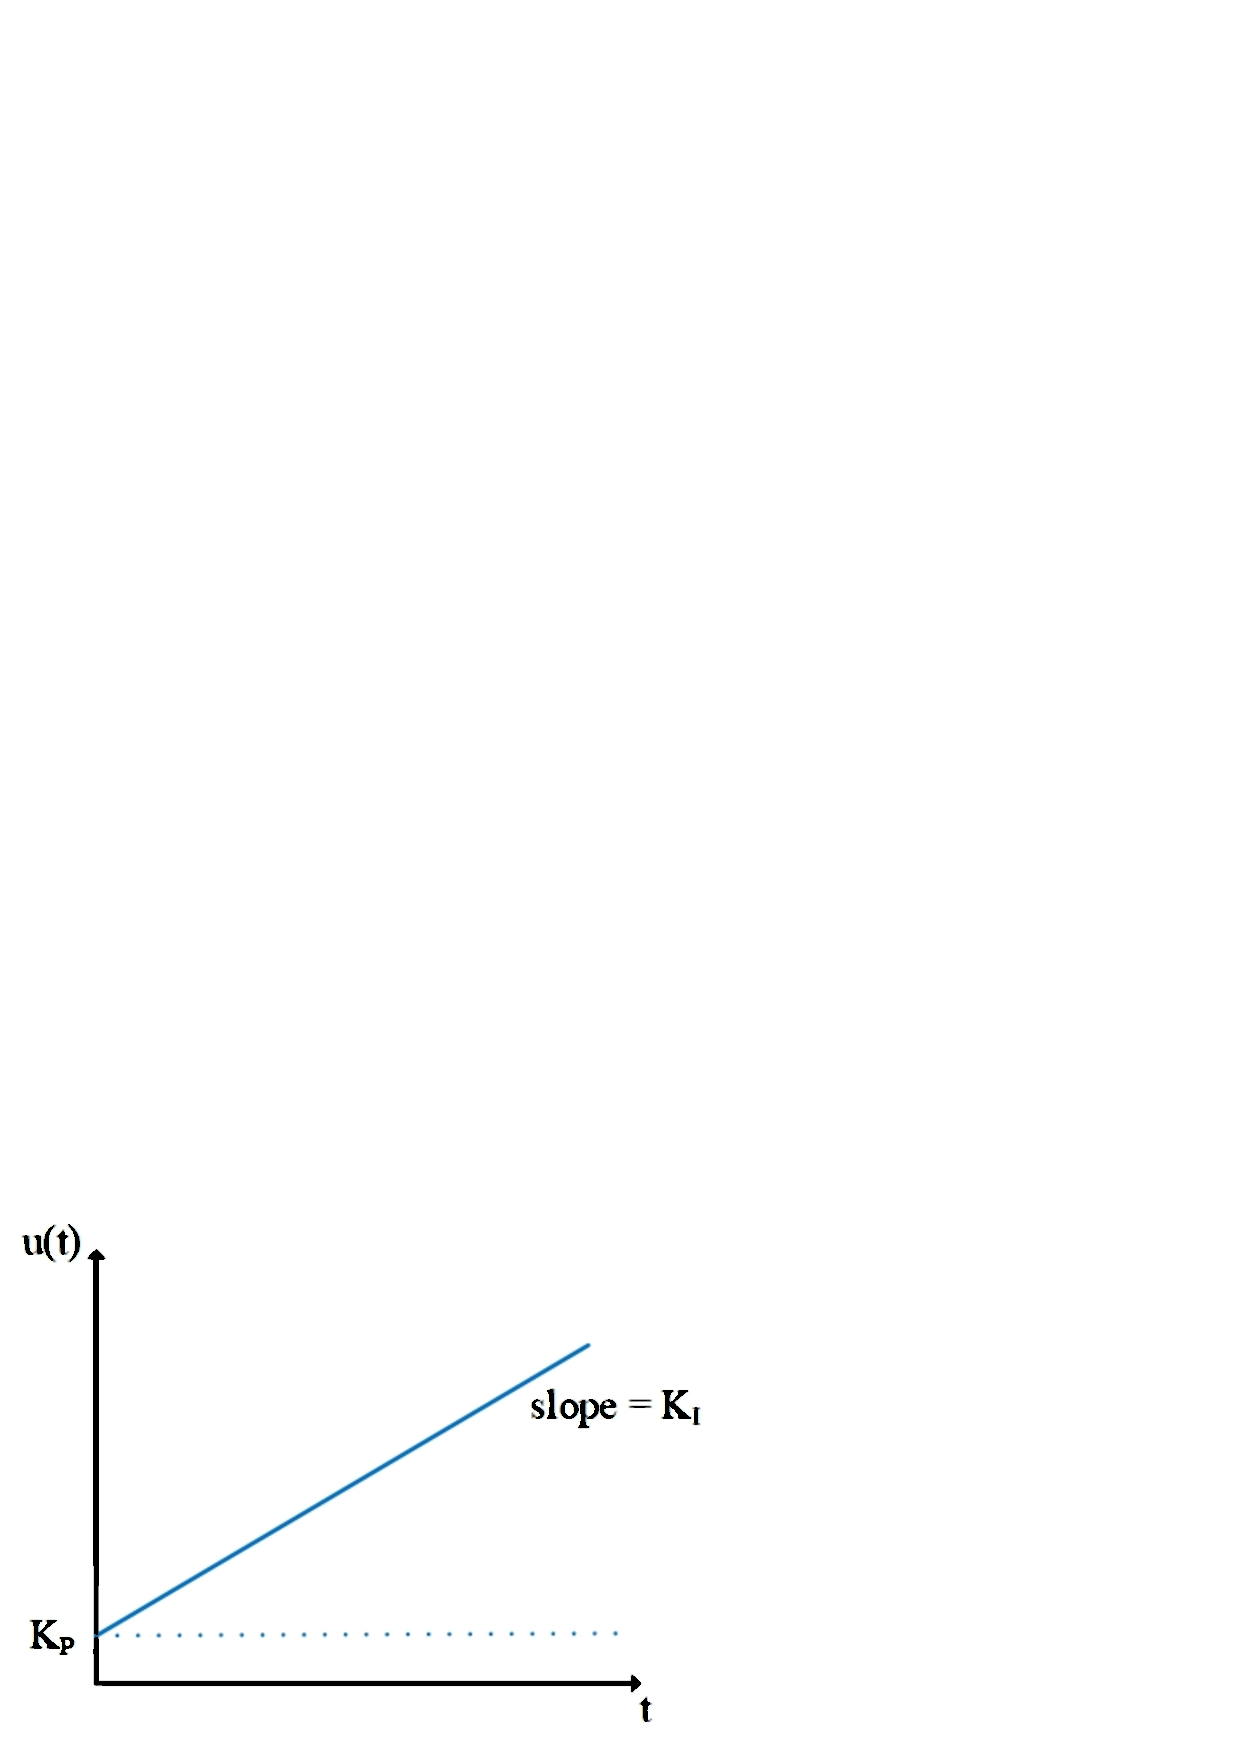
\includegraphics[width=0.4\textwidth]{images/step_resp_pi.jpg}
   \caption[Step response of a PI-Controller]{Step response of a PI-Controller}
   \label{fig:step_resp_pi}
 \end{figure}

\subsection{Tuning rules}
In regards to the controller parameters, tuning is of great importance. If the parameters are chosen incorrectly it can lead to poor performance. There are many different approach to tuning a PI-Controller in order to achieve the best system performance. These are reaching from heuristic methods, over analysis of pole-zero plots, to computer-aided numerical parameter optimization \cite{Reg_10} At this point only the tuning rules according to Ziegler Nichols (ZN) and the rules according to Chien Hrones Reswick (CHR) will be discussed, as these have been used for the implementation of flow control in the practical work.  Information on other approaches can be found in \cite{Reg_11}.

\subsubsection{Tuning rules according to Ziegler Nichols}
The tuning rules according to Ziegler Nichols are on of the most commoly used heuristic methods in tuning controller parameters for PID-Controllers. They are used especially, if a mathematical model of the plant is not available, but the plant can be approximated as a PT$_{n}$-element. \cite{Reg_17}
A necessary condition is that the step response of the plant needs to be experimentally identifiable without risk of damage to the system. After the step response has been determined, it is displayed graphically. Then the inflection tangent is drawn into the step response as shown in the \figurename~\ref{fig:param_zn}.
\begin{figure}
   \centering
   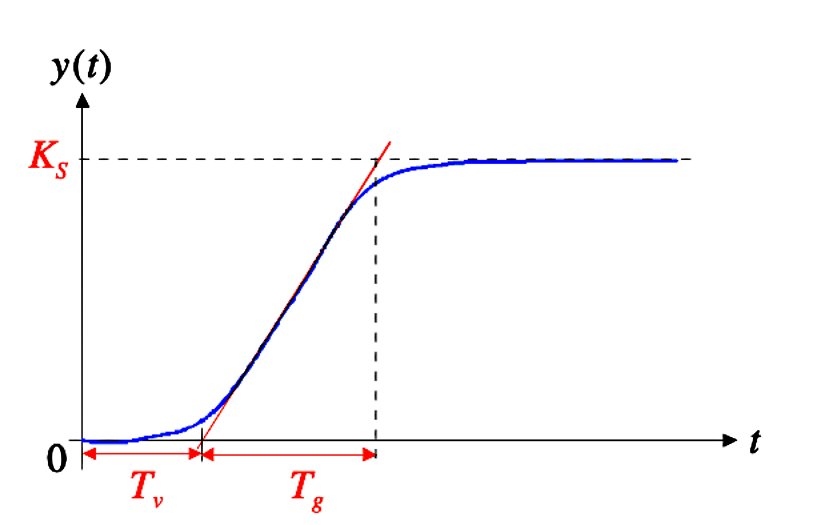
\includegraphics[width=0.8\textwidth]{images/param_zn.jpg}
   \caption[Inflection tangent method Ziegler Nichols]{Inflection tangent method Ziegler Nichols}
   \label{fig:param_zn}
 \end{figure}
The gain $K_{P}$, the delay time $T_{v}$ and the settling time $T_{g}$ can be read from the graph.
The calculation of the controller parameters is performed according to the data in \tablename~\ref{tab:param_zn}. The factor $K_{p}$ from the table equals the term $K_{p}$ in (\ref{eq:pi_contr_2}), while the factor $K_{I}$ is calculated to:
\begin{equation}
    K_{I}  = \frac{K_{P}}{T_{N}}.
 \label{eq:K_I}
\end{equation}
\begin{table}
  \centering
  \begin{tabularx}{0.6\textwidth}{c|c|c|c}
    \toprule
    Controller Type & $K_{P}$ &  $T_{N}$ & $T_{V}$   \\
    \midrule
    P-Controller &  $\frac{T_{G}}{K_{S}T_{v}}$ & $\infty$ & 0 \\
    & & & \\
    PI-Controller & $0.9\frac{T_{G}}{K_{S}T_{v}}$ & $3.33T_{v}$ & 0 \\
    & & & \\
    PID-Controller & $0.9\frac{T_{G}}{K_{S}T_{v}}$ & $2T_{v}$ & $0.5T_{v}$ \\
     \bottomrule
  \end{tabularx}
  \caption[Tuning parameters Ziegler Nichols]{Tuning parameters according to Ziegler Nichols}
  \label{tab:param_zn}
\end{table}

\subsubsection{Tuning rules according to Chien Hrones Reswick}

\section{Iterative Learning Control}

\chapter{Identification}
\section{Sputnik VAD}\label{Sputnik}
% graphic of Sputnik construction
The Sputnik VAD is an axial-flow blood pump, developed in a cooperative project of the National Research University of Electronic Technology, OJSC Zelenograd Innovation-Technology Center of Medical Equipment, FSBI "Academician V.I. Shumakov Federal Research Center of Transplantology and Artificial Organs", Ministry of Health of Russian Federation, DONA-M LLC and BIOSOFT-M LLC in 2009. \cite{Sputnik1}
\\This device is used for left ventricular assistance in patients with acute heart failure. The therapeutic objective in implantation of a Sputnik VAD is bridging to transplantation. The VAD is able to pump up to 10 liters of blood per minute with a continuous flow profile. The implantable pump weighs about $200\, g$, has a length of $81\, mm$ and a maximum diameter of $34\, mm$. It consists of a moving and a stationary part. The moving part, the impeller, a rotor with four blades, contains a permanent NdFeB-magnet, which is actuated by a brushless DC motor. The rotor spins clockwise with speed values between $4000-10000\, rpm$. An overview of the pump's specification is presented in \tablename~ \ref{tab:sput1}.
\begin{table}[ht]
  \centering
  \begin{tabular}{c|c}
    \toprule
    Blood flow  & 0-10 l/min \\
    Rotational speed & 4000-10000 rpm \\
    Length & 81 mm \\
    Diameter & 34 mm \\
    Weight & 200 g \\
    \bottomrule
\end{tabular}
  \caption[Specifications of Sputnik VAD]{Specifications of Sputnik VAD}
  \label{tab:sput1}
\end{table}
\\The stator is located inside a titanium housing with a $16\, mm$ diameter. The stationary part of the pump consists of a flow straightener with three stationary blades and a flow diffusor with three twisted blades. The flow straightener is located in front of the rotor and straightens the incoming blood flow into the rotor. Behind the rotor, blood is directed into the diffusor. %\cite{Sputnik1}
\figurename~ \ref{fig:sput_cross} depicts a cross-section of the Sputnik VAD and identifies its individual components.
The connection between the pump and the cardiovascular system is performed using in- and outflow cannulas, a felt ferule and vascular prosthesis which is sewed to the aorta. \cite{Sputnik1}
\begin{figure}[ht]
  \centering
  \includegraphics[width=0.6\textwidth]{images/chapt_4/sputnik_cross.png}
  \caption[Cross-section of Sputnik VAD \cite{Sputnik6}]{Cross-section of the Sputnik VAD \cite{Sputnik6}.}
  \label{fig:sput_cross}
\end{figure}
\\The Sputnik VAD is powered using two lithium-ion batteries, fully charged providing enough energy for up to eight hours of system support. The maximum charging time for the batteries is less than five hours. During this time the batteries can either be exchanged by another set of batteries or the system can be powered through connection to an AC network. A microprocessor-based driving unit is used to regulate the pump speed, manage the power supply and store parameter data. It is connected percutaneously to the pump with an up to $170\, cm$ long and $5\, cm$ wide lead. \cite{Sputnik1}
\\During the practical part of this work, the pump was controlled using the servo controller module ESCON 50/4 EC-S from maxon motor. This is a 4-quadrant pulse width modulation controller for controlling motors without Hall sensors.
%%%% ANSTEUERUNG ÜBER ESCON ERKLÄREN!!!

\section{Hardware in the Loop Test Bench}
For all measurements and tests performed during this thesis, a hardware in the loop (HiL) test bench of the Chair of Medical Information Technology at RWTH Aachen University was used. The test bench is implemented as a feedback controlled human circulatory system simulator. With the aid of the test rig, it is possible to test MCS systems under various physiological and pathological load patterns of the heart.
\begin{figure}[ht]
  \centering
  \includegraphics[width=\textwidth]{images/chapt_4/mock_loop.jpg}
  \caption[HiL test bench]{Structure of the HiL human ciculatory system simulator based on \cite{MCL}.}
  \label{fig:mock_loop}
\end{figure}
\\The structure of the mock circulatory loop (MCL) is depicted in \figurename~\ref{fig:mock_loop}. The boxes marked $V_{1}$ and $V_{2}$ are pressure compartments simulating the volume of the left ventricle and the aorta, respectively. Therefore, the pressure values of these compartments, referred to as $p_{1}$ and $p_{2}$, can be physiologically compared to the pressure values of the left ventricle and aorta. The MCL is actuated by three gear pumps ($GP_{1}$, $GP_{12}$ and $GP_{2}$) and two voice coil actuators ($VCA_{1}$ and $VCA_{2}$). The Sputnik VAD is connected to the pressure chambers in parallel, enabling tests similar to real use cases. This way, the VAD can be subjected to comparable pressure changes in the differential pressure between the aorta and ventricle as would be the case when used on the beating heart.
\\By controlling the MCL through a dSpace system (DS1103), pressure in the chambers can be adjusted in real time to simulate different cardiac dysfunctions. The dSpace system furthermore enables recording of reference signals presented to the MCL, as well as real time measurements. All recorded data can be exported formatted as Matlab matrices.
\\As the Sputnik VAD is not usually included into the MCL setup, flow through the device can not be measured without further equipment. For this purpose the Transonic Systems Inc. T110 flowmeter is included in the setup. The flow sensor measurement is based on ultrasonic technology. The sensor probe, as presented in \figurename~\ref{fig:flow_meter_tube}, is mounted onto the tube leading from the pressure chamber representing the left ventricle to the VAD. The flowmeter also is connected to the dSpace system, enabling recording of the measured flow values. In \figurename~\ref{fig:mock_loop} the measurement of the device is represented by $\dot{V}_{DUT}$.
\begin{figure}[ht]
  \centering
  \includegraphics[width=0.8\textwidth]{images/chapt_4/flow_meter.pdf}
  \caption[Sputnik VAD and flowmeter in HiL setup]{Sputnik VAD and flowmeter in HiL setup.}
  \label{fig:flow_meter_tube}
\end{figure}
\\The ESCON servo controller mentioned in chapter \ref{Sputnik}, as well as the other devices, is connected to the dSpace system. Using the digital input port of the controller, a set value for regulation of the rotational speed can be transferred to the controller after setting the value in the system.
\\The dSpace system itself is controlled with the use of the program ControlDesk. This software provides the opportunity to include Matlab and Simulink source code. By this, controllers designed with the use of Simulink can directly be tested at the HiL test bench.

\section{System Identification}
For the implementation of flow control algorithms for the Sputnik VAD, knowledge of the system behavior is required. In order to gain this information, various tests have been performed to determine a static map for the system. For this purpose, a multiple-input-single-output (MISO) system with input variables differential pressure $\Delta{p}$ in $mmHg$, rotational speed $v$ in $rpm$ and output variable blood flow $q$ in $l/min$ is assumed. The differential pressure is defined as
\begin{equation}
  \Delta{p} = p_{ao} - p_{lv} = p_2 - p_1,
\end{equation}
with $p_{ao}$ depicting the pressure of the aorta and $p_{lv}$ the left ventricular pressure.
\\Using the HiL test rig, the differential pressure was increased in steps of $20\, mmHg$ starting at $0\,mmHg$ and ending at $140\,mmHg$. For each differential pressure step, the reference speed of the pump was increased from $4000\, rpm$ in steps of $1000\, rpm$ to $9000\, rpm$. Flow for each reference speed was measured for $5\, s$. In order to eliminate inaccuracies due to transient processes, solely the last quarter each mesurement stage was considered for the evaluation using Matlab. \figurename~\ref{fig:test_60w40g_long} depicts the signal curves for the measurement described above. The upper graph shows the course of the reference differential pressure ($\Delta{p_{ref}}$) and the differential pressure measured at the HiL test stand ($\Delta{p_{HiL}}$).
In the middle, the curves of the reference velocity ($v_{ref}$) and the measured velocity of the Sputnik VAD ($v_{vad}$) are shown. The lower graph shows the resulting flow through the blood pump ($q_{vad}$).


\begin{figure}[ht]
  \centering
  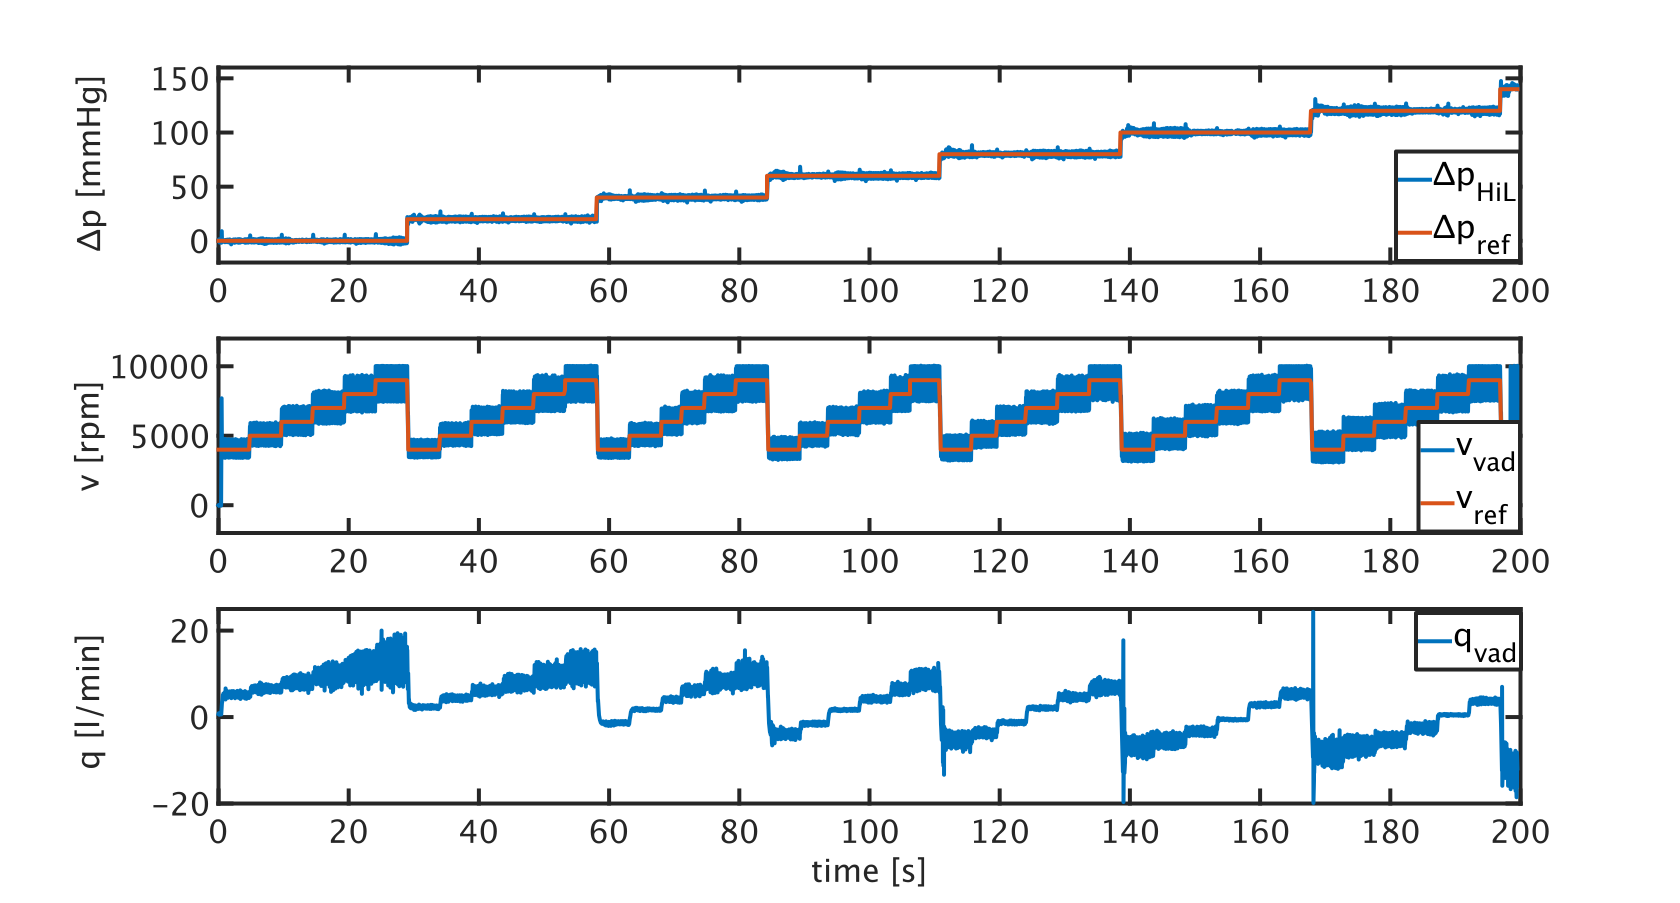
\includegraphics[width=\textwidth]{images/chapt_4/Test_60w40g_long.pdf}
  \caption[Signal curves for creation of the static map.]{Signal curves for creation of the static map for $60\,\%$ water, $40\,\%$ glycerin solution with $15 \, cm$ long tubes. Top: differential pressure, middle: rotational speed, bottom: flow through VAD.}
  \label{fig:test_60w40g_long}
\end{figure}
To determine the static map, the flow data is first broken down into individual parts corresponding to the various differential pressure levels.  These are then split into data sections for each velocity rate. Finally, the mean of the last quarter of each section is calculated. The average flow values are then displayed as a function of the differential pressure. The values of each velocity level are connected with each other.
\\At the beginning of the practical work, the Sputnik VAD was connected to the test stand via tubes of about $30\, cm$ length on both sides. Since in clinical use, the pump is implemented in the patient's body and connected to the left ventricle and aorta, the tube length is not representative of a real application. To test the effect tube length has on the operating range of the pump, three different tube lengths for attachment of the VAD to the test rig are compared. The measurements have been performed with tubes of approximately $5\, cm$, $10\, cm$ and $15\, cm$ length. \figurename~\ref{fig:60w_40g} depicts the static maps for all three tube lengths measured with a fluid solution of $60\, \%$ water $40\, \%$ glycerin.
\begin{figure}[ht]
  \centering
  \includegraphics[width=\textwidth]{images/chapt_4/60w40g_tube_length_new.pdf}
  \caption[Static map for different tube length in 60 \% water 40 \% glycerin solution]{Static map for varying tube length in 60 \% water 40 \% glycerin solution.}
  \label{fig:60w_40g}
\end{figure}
\\Under inspection of the blue curves corresponding to a tube length of $5\, cm$ it is evident that measurements in this case were only performed up to a differential pressure of $\Delta{p}=100 \, mmHg$. This is a result of the abrupt change in differential pressure and reference speed which lead to spontaneous reduction of the flow and possibly high backflow values through the pump. As a result, the pump's rotor comes to a stop. For longer tubes ($10\, cm$ and $15\, cm$ length) and therefore higher flow resistance, this phenomenon occurs at a differential pressure $\Delta{p}=140\, mmHg$. However, the deviation of the curves is insignificant when comparing all three cases. Due to this the tubes of $15\, cm$ length were chosen for reasons of improved handling of the MCL. \figurename~\ref{fig:anh_1} to \figurename~\ref{fig:anh_3} in the appendix show comparisons of the static maps for varying tube length in different mixing ratios of water and glycerin.
\\In addition to different tube lengths, another preliminary investigation was carried out with regard to the influence of the test liquid used. Since leakage or evaporation of test liquid can occur in some parts, it is relevant to know the effect a change in liquid conditions has on the test performance. The same measurements for determining the static map were performed in pure water, a solution of $80\, \%$ water $20\, \%$ glycerin, a solution of $60\, \%$ water $40\, \%$ glycerin and a solution of $40\, \%$ water $60\, \%$ glycerin. Representing the static maps for all four solutions measured, \figurename~\ref{fig:long_tubes} discloses significant deviations between the fluids.
\begin{figure}[ht]
  \centering
  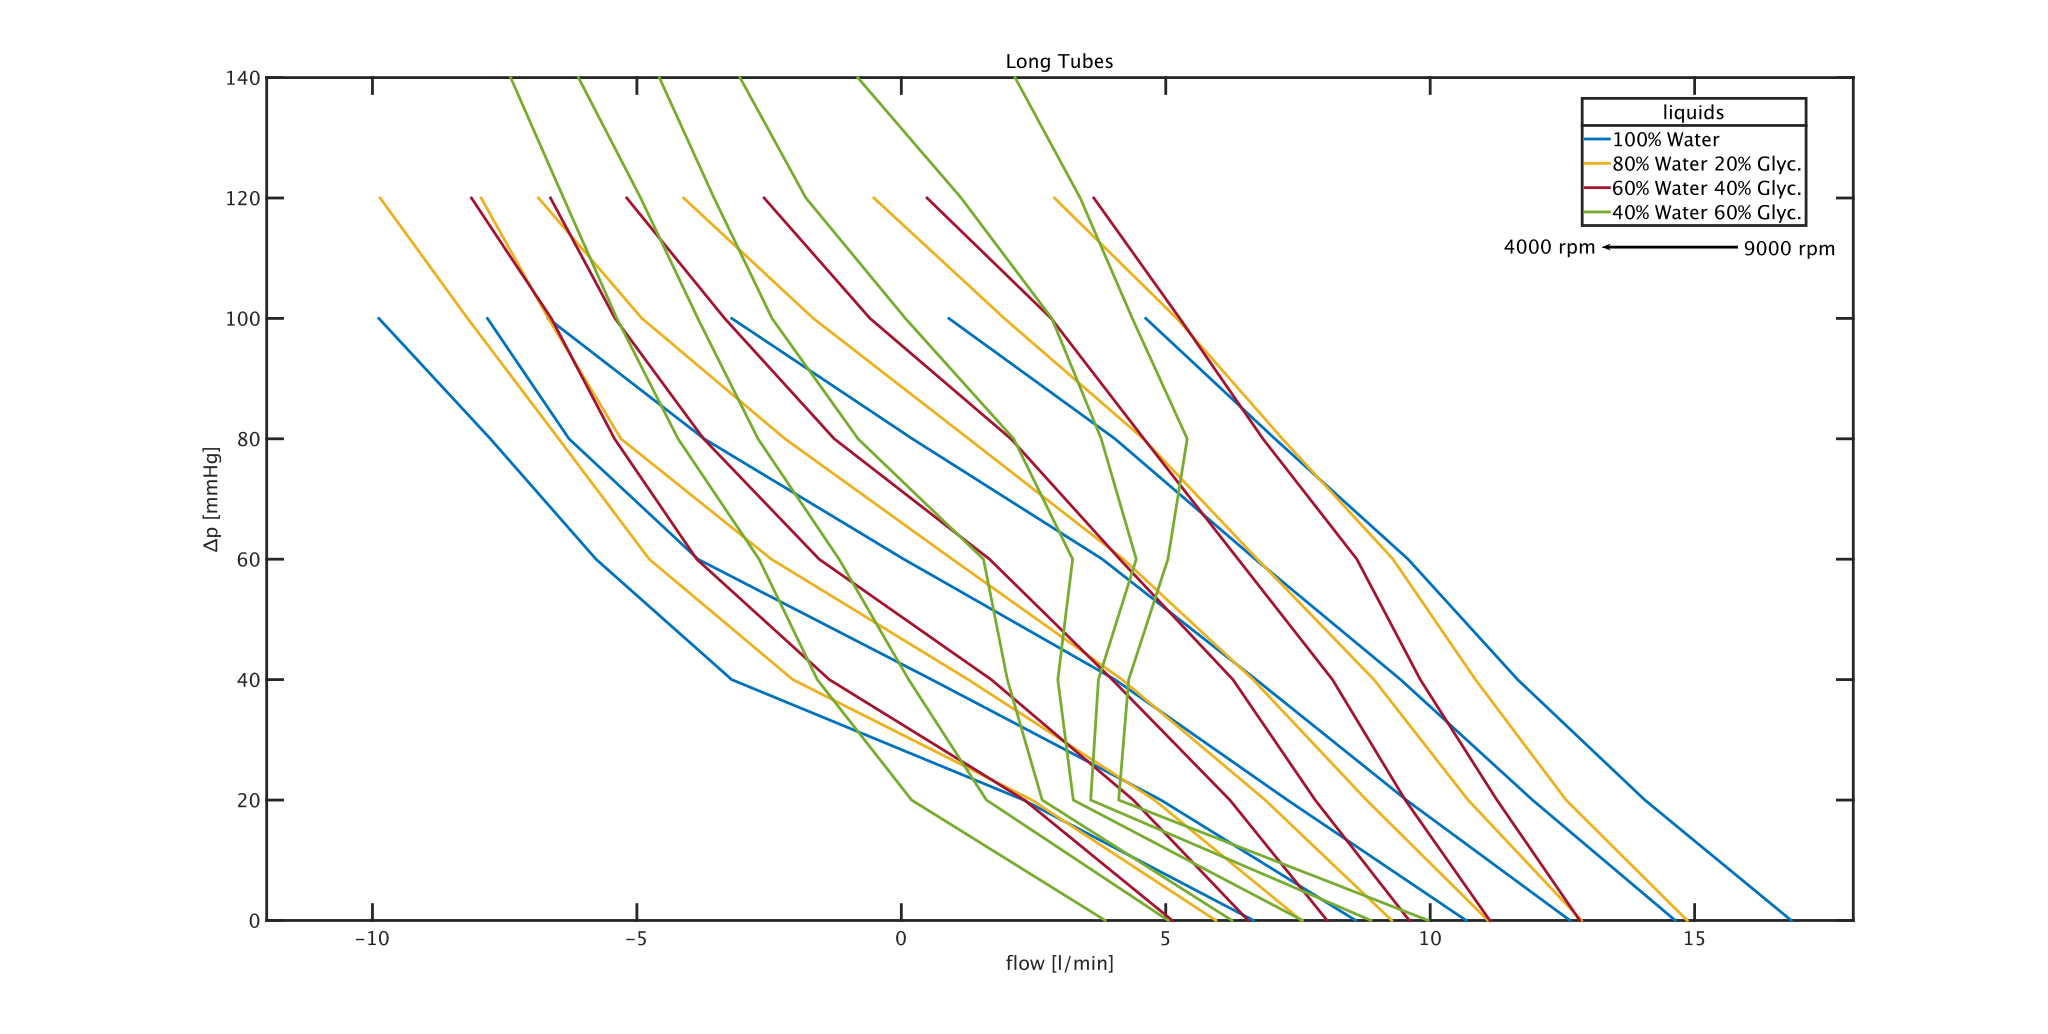
\includegraphics[width=\textwidth]{images/chapt_4/long_liquid_change_new.pdf}
  \caption[Static map for varying fluid solution with $15\,cm$ long tubes]{Static map for varying fluid solutions with $15\,cm$ long tubes.}
  \label{fig:long_tubes}
\end{figure}
 \\Since the resistance of the liquid falls with decreasing proportion of glycerin in the solution, differences in reachable differential pressure occur due to the aforementioned reason of spontaneous flow reduction. However, as the fluid resistance increases, the pumpable flow decreases. All further measurements of this thesis are performed for a solution of $60\, \%$ water $40\,\%$ glycerin as this mixture most closely reflects the properties of blood.
\figurename~\ref{fig:anh_4} and \figurename~\ref{fig:anh_5} in the appendix depict comparisons of the static maps for varying  solutions with $5\, cm$ and $10\, cm$ tube length.
The resulting static map for the chosen final setup of the MCL is depicted in \figurename~\ref{fig:60w40glong}.

\begin{figure}[ht]
  \centering
  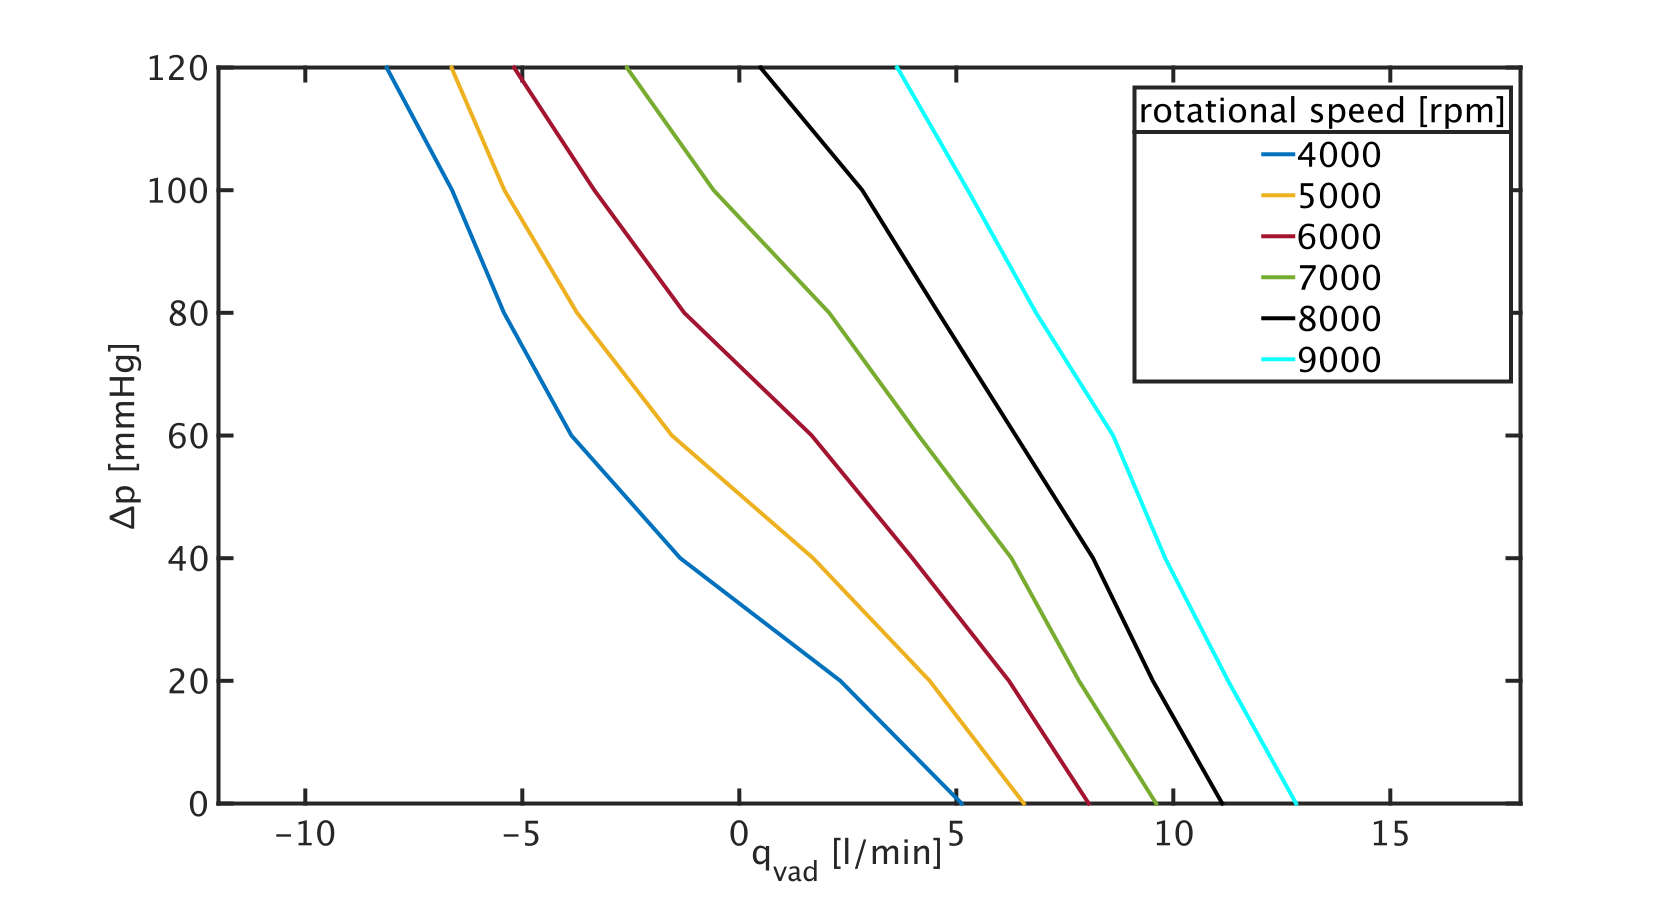
\includegraphics[width=\textwidth]{images/chapt_4/60w40g_long.pdf}
  \caption[Static map for solution of $60\, \%$ water $40\, \%$ glycerin with $15\,cm$ long tubes]{Static map for solution of $60\, \%$ water $40\, \%$ glycerin with $15\,cm$ long tubes.}
  \label{fig:60w40glong}
\end{figure}

%% close up von einem 1k Sprung zur Auslegung der Plant im durch 4.7 definitierten positiven Fluss Bereich.
%% Vergleich des gemessenen Signals mit simuliertem Signal.
As part of the system identification, the transfer function of the Sputnik VAD is determined. For this purpose, the step response of the pump to a $1000\,rpm$ step in reference speed is analyzed.
\\Initially, the measured flow values from the static map determination measurement are prepossessed by using a $2^{nd}$-order butterworth filter with a cut-off frequency of $f_c = 5\,Hz$ and sampling frequency $f_s=1000 \, Hz$. For determination of the transfer function, filtered flow for an increase from $v_{ref,low}=5000\,rpm$ to $v_{ref,high}=6000\,rpm$ in reference speed at a differential pressure of $\Delta{p}=40\,mmHg$ is analyzed. The blue line in \figurename~\ref{fig:plant} depicts the filtered flow for this measurement. It is evident that the system's behavior can be approximated by a $PT_1$-element.
 The characteristic parameters of the transfer function according to equation (\ref{eq:tf_pt1}) are represented in \figurename~\ref{fig:plant}. The static gain $k_s$ is determined as
\begin{equation}
%  \begin{split}
  k_s = \frac{k_{high}-k_{low}}{v_{ref,high}-v_{ref,low}}=0.0018
  %\\ = \frac{2.3008 - 0.4672}{6000 - 5000} = 0.0018.
%  \end{split}
\label{eq:k_s_1}
\end{equation}
with $k_{high}=2.3008$ and $k_{low}=0.4672$. The time constant T is determined to $T=0.081$.
According to equation (\ref{eq:tf_pt1}) the transfer function for the plant results in
\begin{equation}
    G(s) = \frac{0.0018}{1+0.081s}.
 \label{eq:plant}
\end{equation}
\begin{figure}[t]
  \centering
  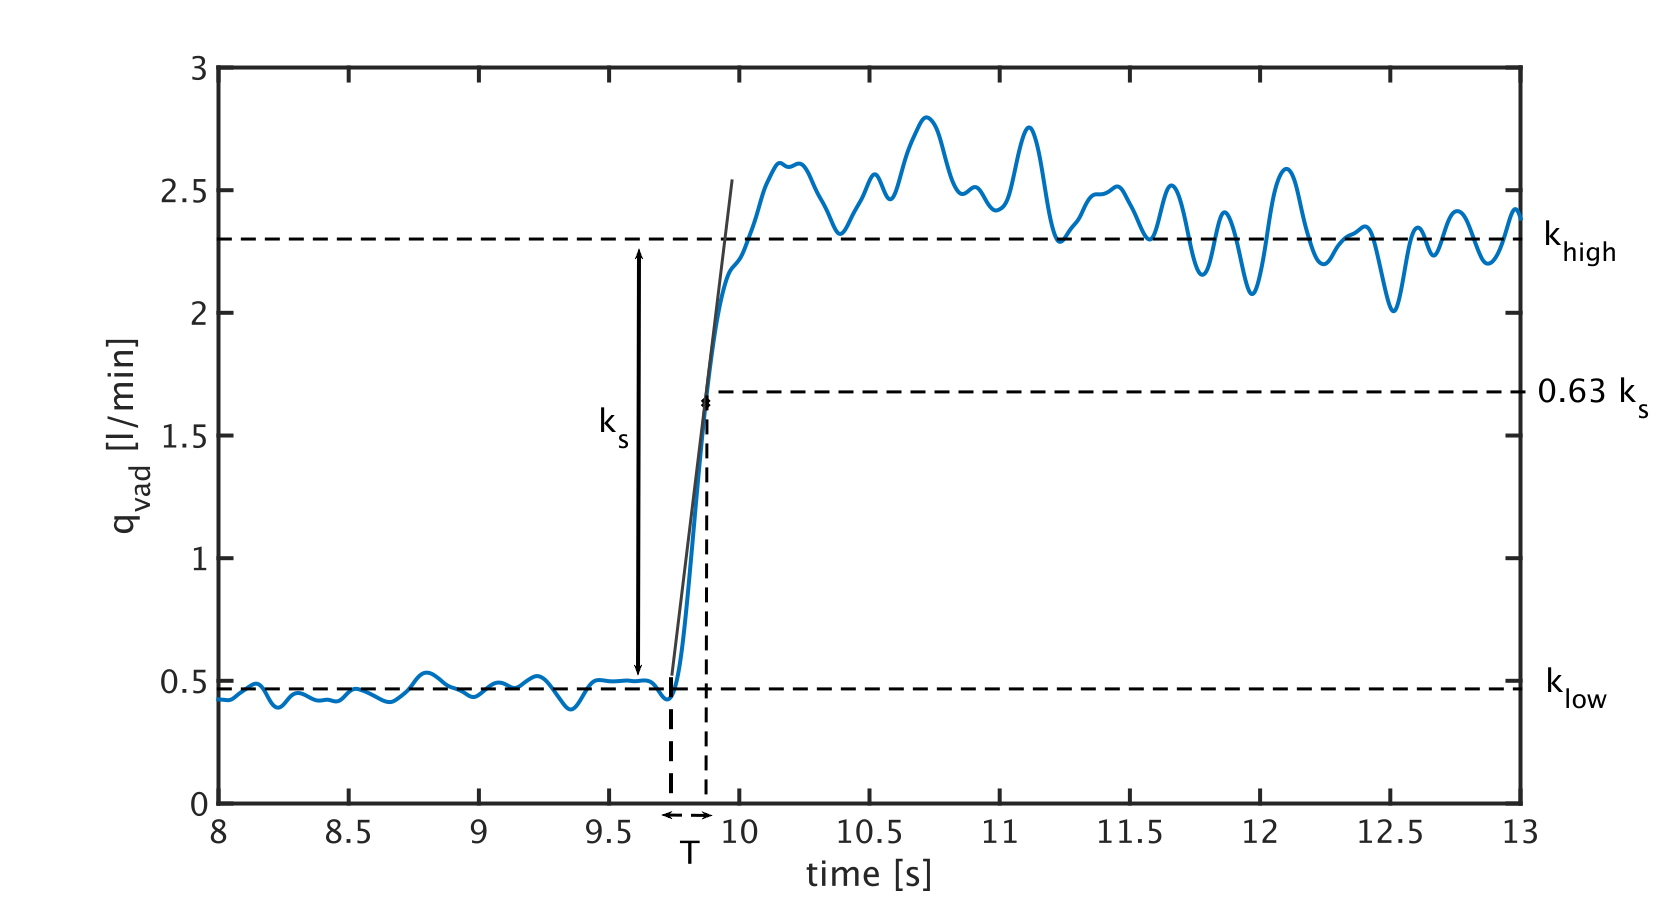
\includegraphics[width=\textwidth]{images/chapt_4/plant_generation.pdf}
  \caption[Transfer function of Sputnik VAD]{Step in flow, triggered by a step in reference speed by 1000 rpm with identification of the variables for determining the transfer function of a $PT_1$ element.}
  \label{fig:plant}
\end{figure}

\chapter{Flow Control}
In this chapter, implementation and evaluation of various control algorithms for flow control purposes will be presented. At first, the aim is to enable regulation of flow to a constant value. Later on, the system's ability to follow different reference flow trajectories will be tested. In a final step, the system will be subjected to disturbancees through the HiL test rig in form of heart beats at different heart rates. Performances of the implemented control algorithms will be compared.

% As a first step towards flow control implementation two versions of PI controllers are implemented to ensure stable system behavior. After comparing the performance results of both approaches, a parallel approach to ILC implementation under use of the higher performing PI controller is applied to improve the follow up behavior and reduce control errors.

\section{PI Controller}
PI control implementation is performed on the basis of the tuning rules according to Ziegler Nichols (see chapter \ref{chap:ZN}) as well as according to Chien Hrones Reswick (Chapter \ref{chap:CHR}). The performance of these controllers is then compared and evaluated.

\subsection{Design and Implementation}
As a preparation for utilization of the inflection tangent method for these tuning approaches, a measurement similar to the one for determining the static map is performed. \figurename~\ref{fig:dyn_meas} depicts the signal curves for the determination of the tuning parameters.
\begin{figure}[ht]
  \centering
  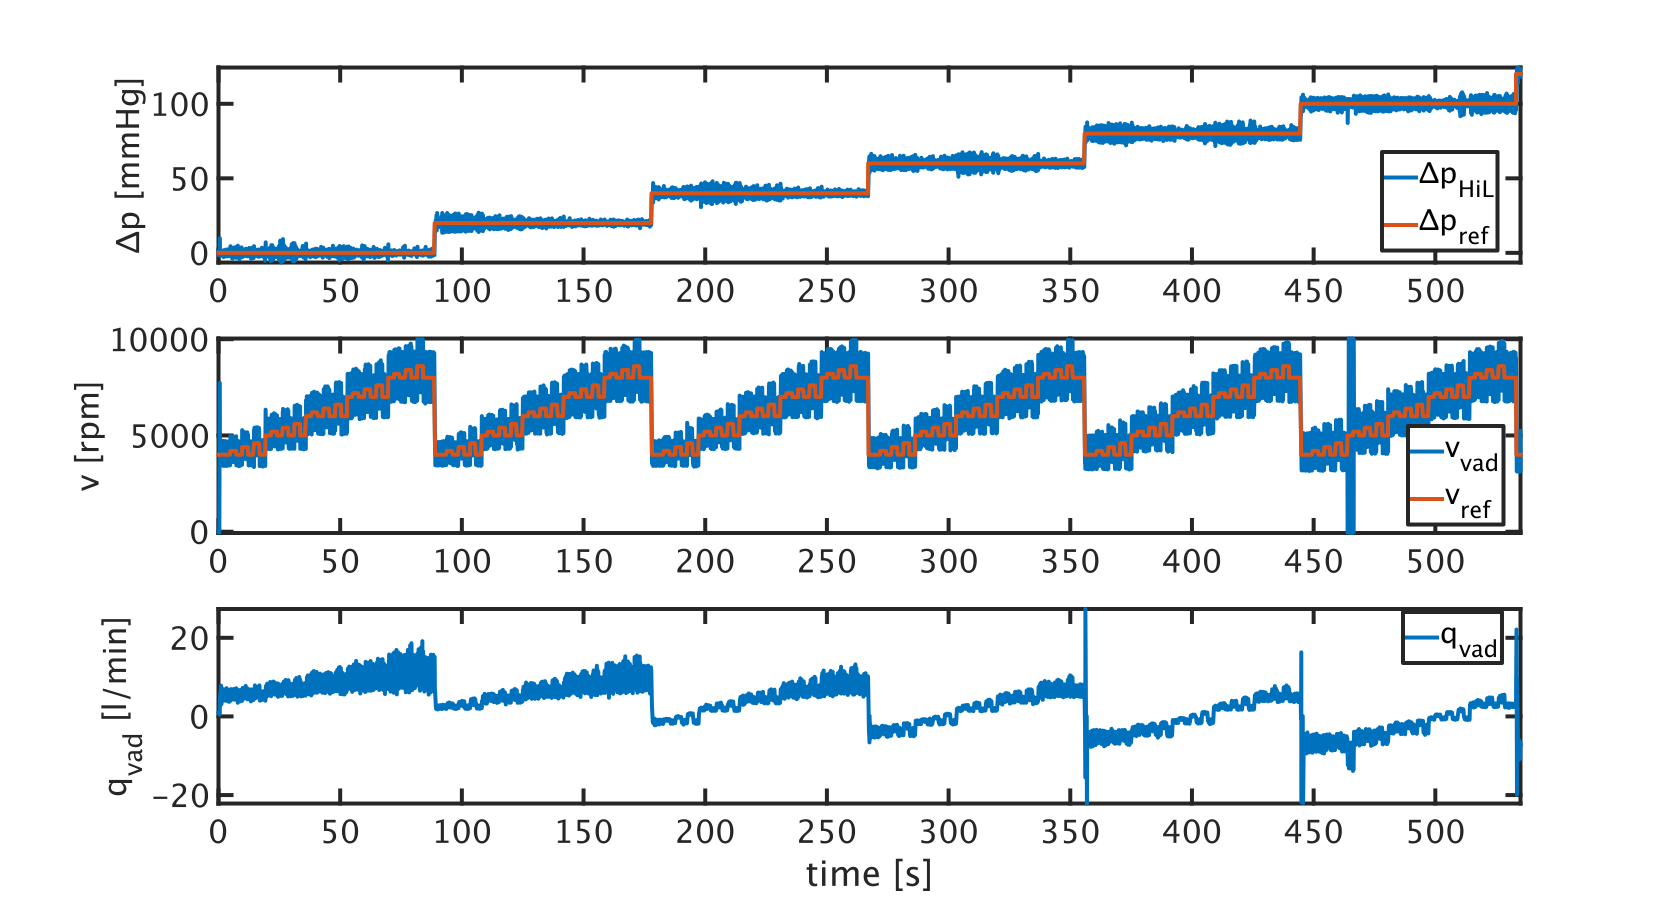
\includegraphics[width=\textwidth]{images/chapt_5/dyn_measure.pdf}
  \caption[Signal curves for determination of PI controller parameters]{Signal curves for determination of PI controller parameters. Top: differential pressure as reference and measured signal, middle: reference and measured rotational speed, bottom: measured flow through Sputnik VAD.}
  \label{fig:dyn_meas}
\end{figure}
As presented in the upper graph, differential pressure is increased in steps of $20\,mmHg$ from $\Delta{p}=0\,mmHg$ to $\Delta{p}=100mmHg$. For each level the sequence of reference velocities depicted exemplary for $\Delta{p}=40\,mmHg$ in the center graph of \figurename~\ref{fig:dyn_meas_40} is targeted. Starting at $v_{ref}=4000 \, rpm $ the velocity, in three steps of varying height, is first increased and then decreased by the same value. The first step amounts to $200 \, rpm$, the second to $400\,rpm$ and the third to $600 \, rpm$. The reference value is then increased by $1000\,rpm$ and again the three steps are executed. This sequential behavior is repeated up to a start value of $v_{ref}=8000\,rpm$.
\begin{figure}[ht]
  \centering
  \includegraphics[width=\textwidth]{images/chapt_5/dyn_meas_40.pdf}
  \caption[Signal curves for determination of PI controller parameters at $\Delta{p}=40\,mmHg$]{Signal curves for determination of PI controller parameters at $\Delta{p}=40\,mmHg$.}
  \label{fig:dyn_meas_40}
\end{figure}
For the determination of the parameters for the controller design the step from $v_{ref,low}=5000\, rpm$ to $v_{ref,high}=5400\, rpm$ at $\Delta{p}=40mmHg$, which is located in the center of the pump's operating range, is used.
Since the flow signal is affected by high measurement noise, the signal is prepossessed using an $8^{th}$-order butterworth filter with cut off frequency $f_c=5\,Hz$ and sampling frequency $f_s=1000\,Hz$.
\begin{figure}[ht]
  \centering
  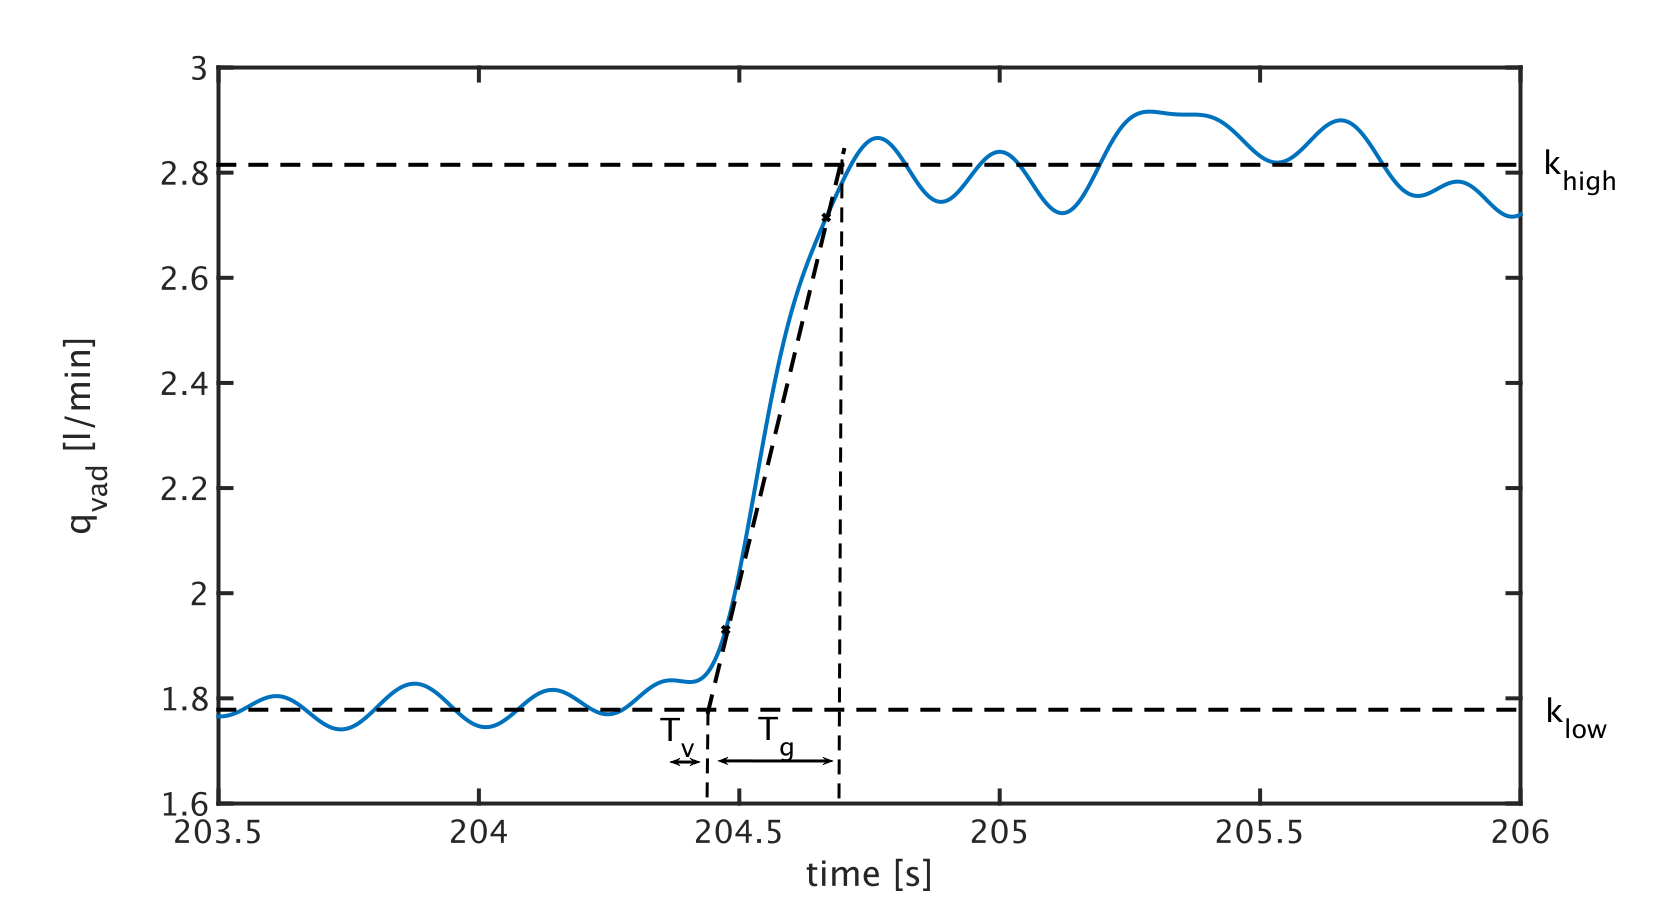
\includegraphics[width=\textwidth]{images/chapt_5/param_calc_PI.pdf}
  \caption[Step response for determination of PI controller tuning parameters]{Step response for a step in rotational speed of $400\,rpm$ for determination of PI controller tuning parameters.}
  \label{fig:param_calc_PI}
\end{figure}
The resulting signal and the characteristic parameters needed for parameter tuning of the PI controller are depicted in \figurename~\ref{fig:param_calc_PI}. With $k_{high}=2.8149$ and $k_{low}=1.7783$ the static gain is determined as in equation (\ref{eq:k_s_1}) to
\begin{equation}
  k_s = \frac{k_{high}-k_{low}}{v_{ref,high}-v_{ref,low}}= 0.0026.
\label{eq:k_s_2}
\end{equation}
The time constants result to $T_g=0.193$ and $T_v=0.1$.
\\For determination of a PI controller tuned according to Ziegler Nichols equations (\ref{eq:kp_zn}) to (\ref{eq:T_N_zn}) are used. By this $K_{P}$ is determined as
\begin{equation}
  K_{P} = 0.9*\frac{0.193}{0.0026*0.1}=670.3052
\end{equation}
and $K_I$ as
\begin{equation}
  K_{I}  = \frac{670.3052}{3.3*0.1}=2031.2278.
\end{equation}
Substituting these values in equation (\ref{eq:pi_contr_2}) results in the transfer function
\begin{equation}
  G_{PI,ZN}(s)=670.3052+\frac{2031.2278}{s}.
\end{equation}
\\The calculation for overdamped controller behavior was chosen for the controller tuning using Chien Hrones Reswick. Determination of the parameters $K_P$ and $K_I$ is performed following the equations presented in \tablename~\ref{tab:param_chr} resulting in
\begin{equation}
  K_P = 0.35*\frac{0.193}{0.0026*0.1}=260.6742
\end{equation}
and
\begin{equation}
  K_I = \frac{260.6742}{1.2*0.1}=2172.2853.
\end{equation}
This in turn leads to the transfer function
\begin{equation}
  G_{PI,CHR}(s)=260.6742+\frac{2172.2853}{s}.
\end{equation}
\subsection{Evaluation}
% gesamt:
% rms pi total chr = 0.3705
% rms pi total zn = 0.5396
% \begin{figure}[ht]
%   \centering
%   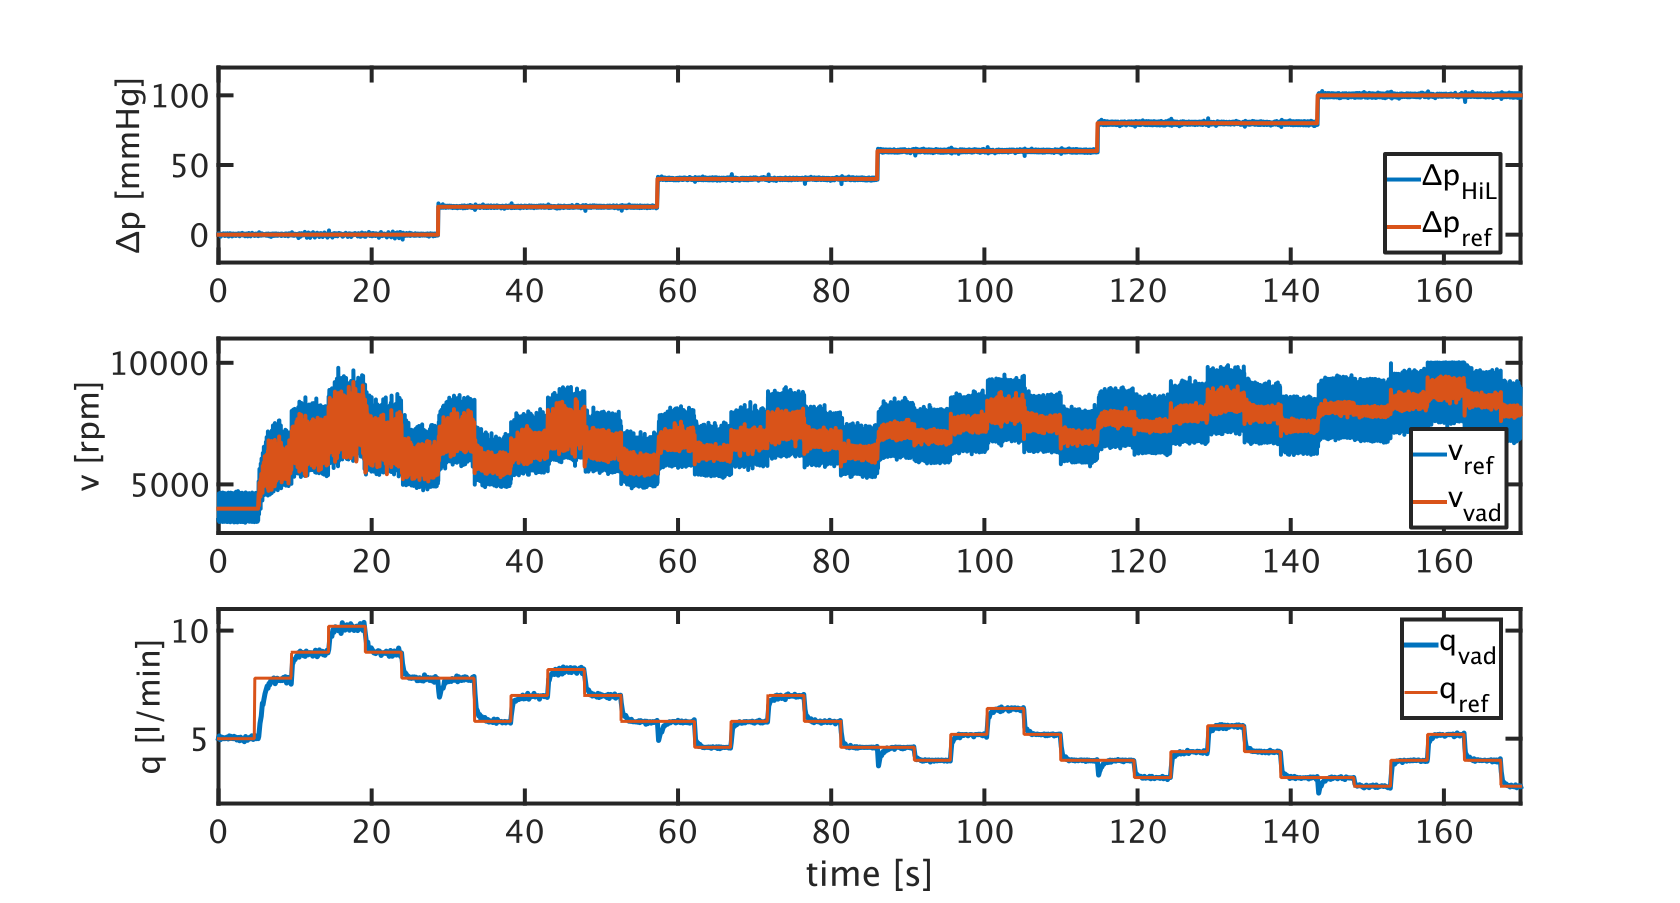
\includegraphics[width=\textwidth]{images/chapt_5/pi_contr_chr.pdf}
%   \caption[Step response for determination of PI controller tuning parameters]{Step response for a step in rotational speed of $400\,rpm$ for determination of PI controller tuning parameters.}
%   \label{fig:pi_contr_chr}
% \end{figure}

% \begin{figure}[ht]
%   \centering
%   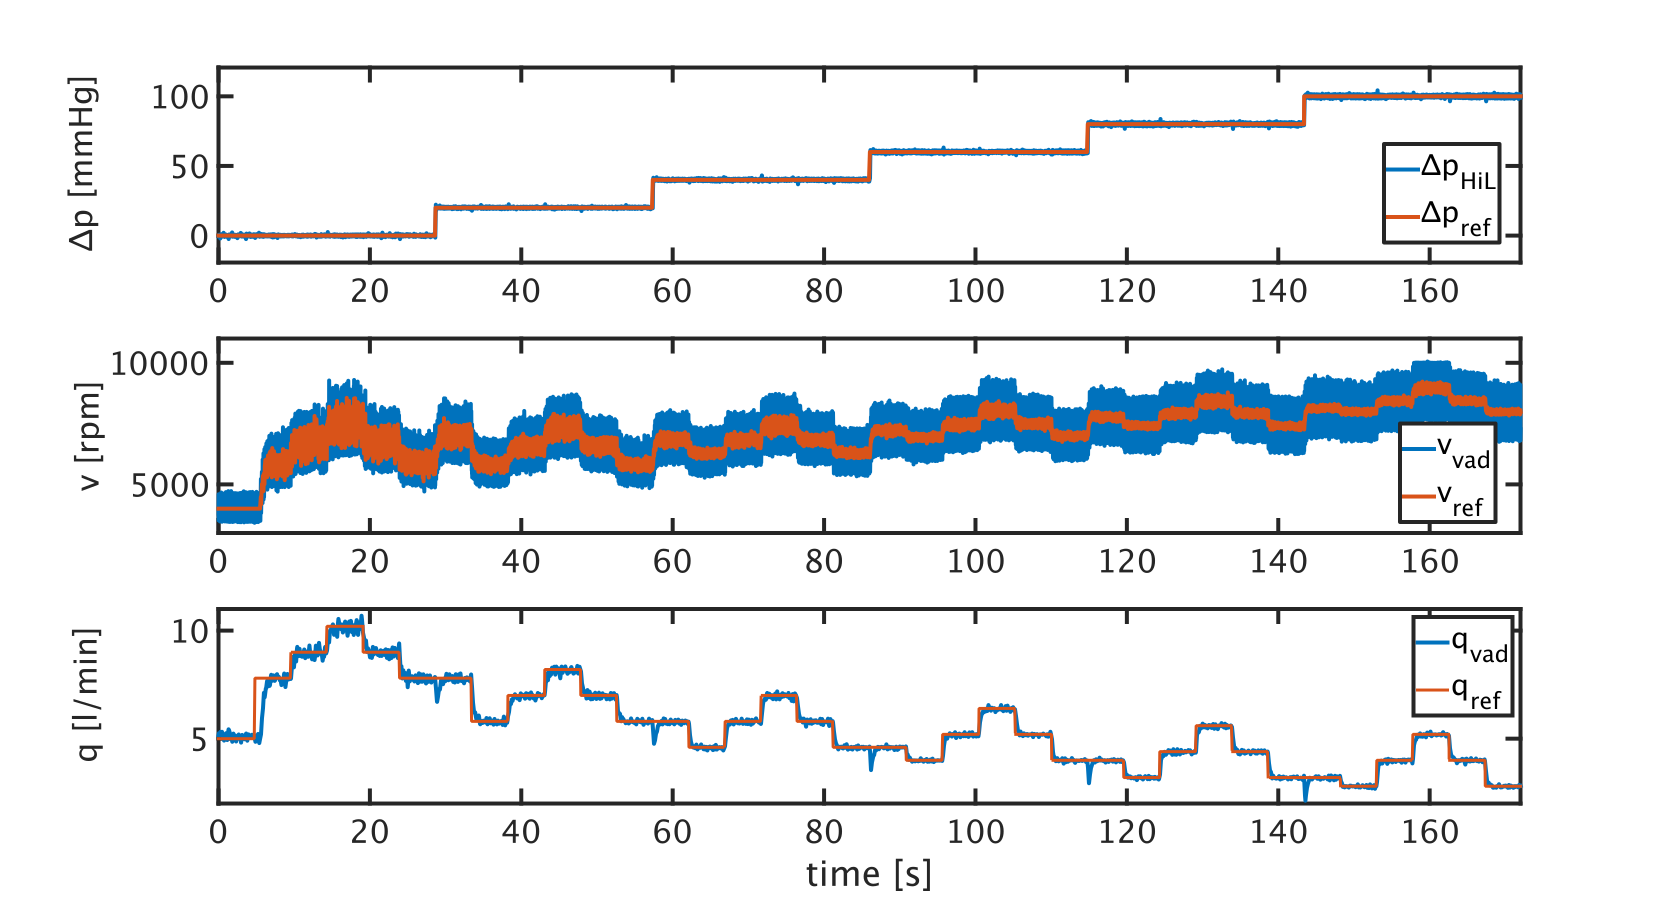
\includegraphics[width=\textwidth]{images/chapt_5/pi_contr_zn.pdf}
%   \caption[Step response for determination of PI controller tuning parameters]{Step response for a step in rotational speed of $400\,rpm$ for determination of PI controller tuning parameters.}
%   \label{fig:pi_contr_zn}
% \end{figure}

% Bereich der Auslegung: 40mmHg
% RMS PI CHR = 0.2753
% RMS PI ZN = 0.4013

% \begin{figure}[ht]
%   \centering
%   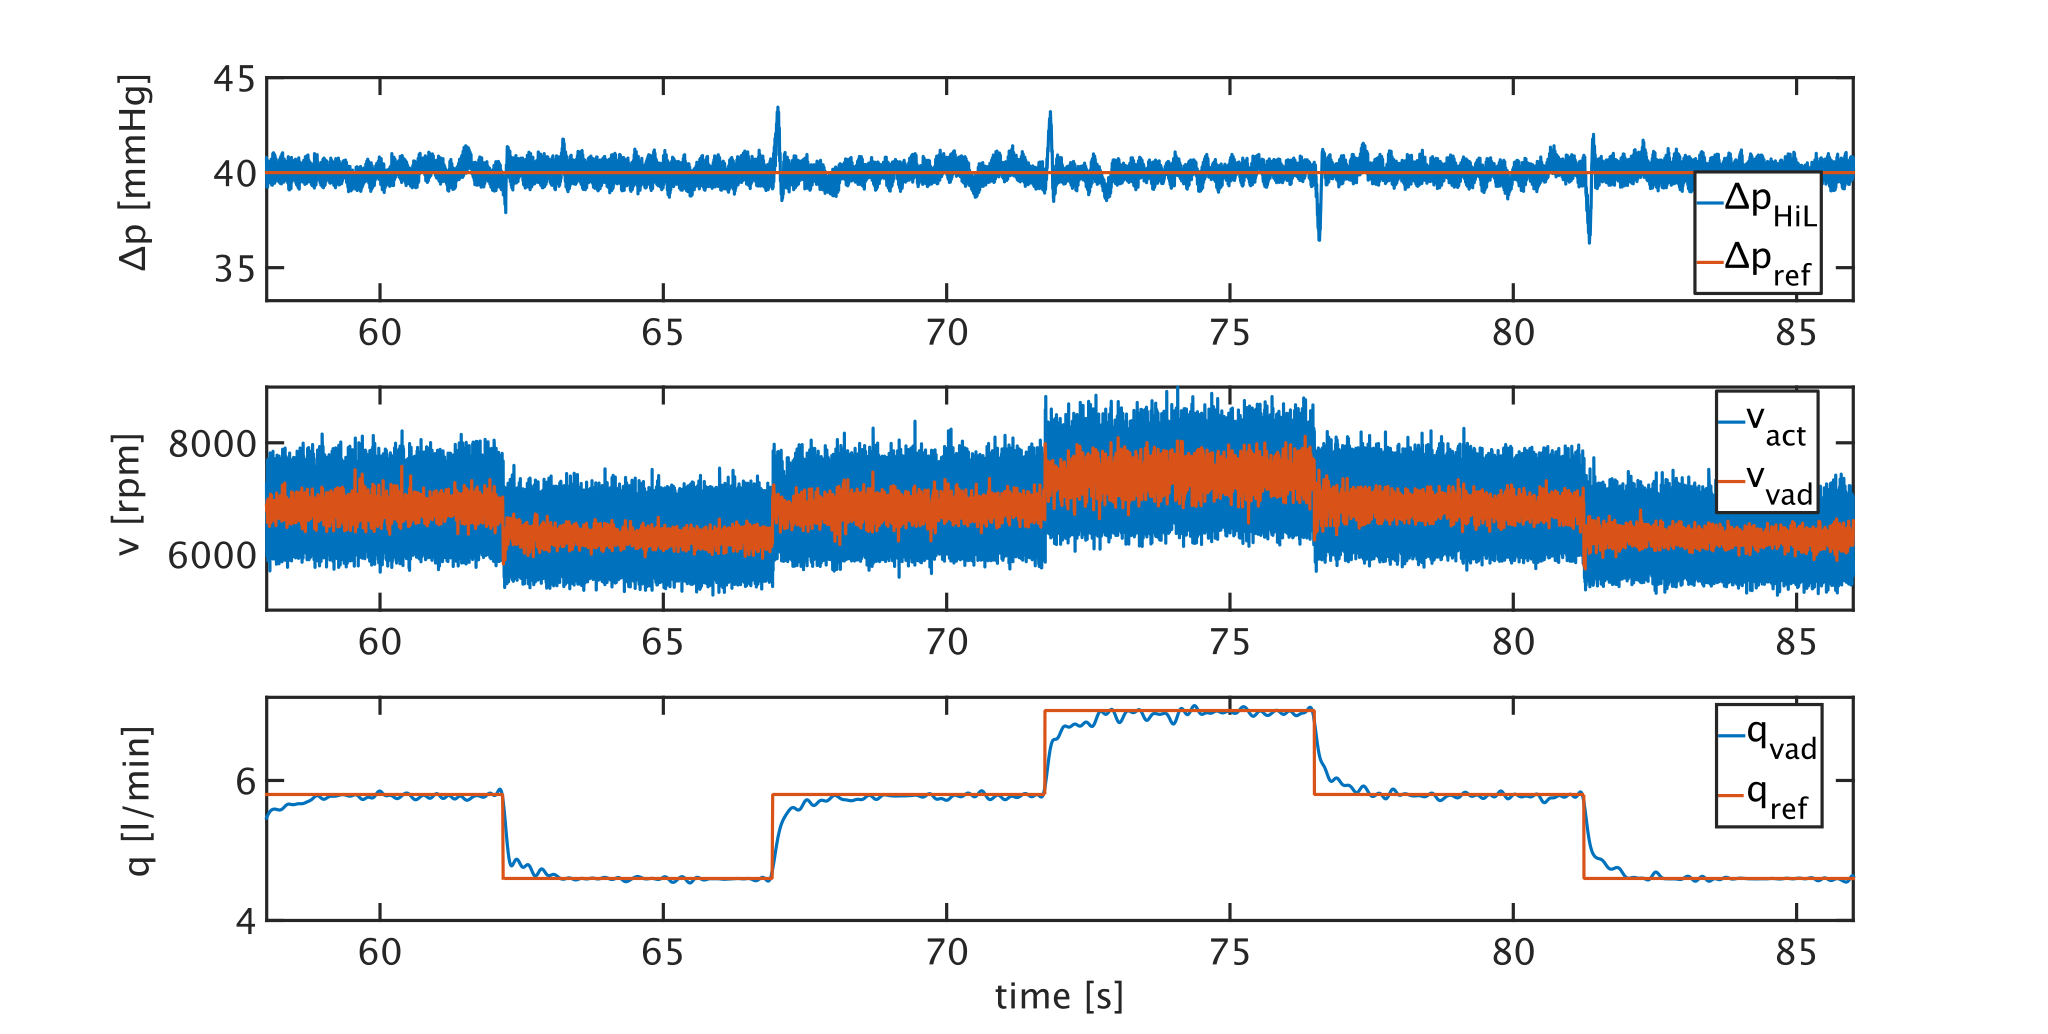
\includegraphics[width=\textwidth]{images/chapt_5/pi_contr_chr_40.pdf}
%   \caption[Step response for determination of PI controller tuning parameters]{Step response for a step in rotational speed of $400\,rpm$ for determination of PI controller tuning parameters.}
%   \label{fig:pi_contr_chr_40}
% \end{figure}

% \begin{figure}[ht]
%   \centering
%   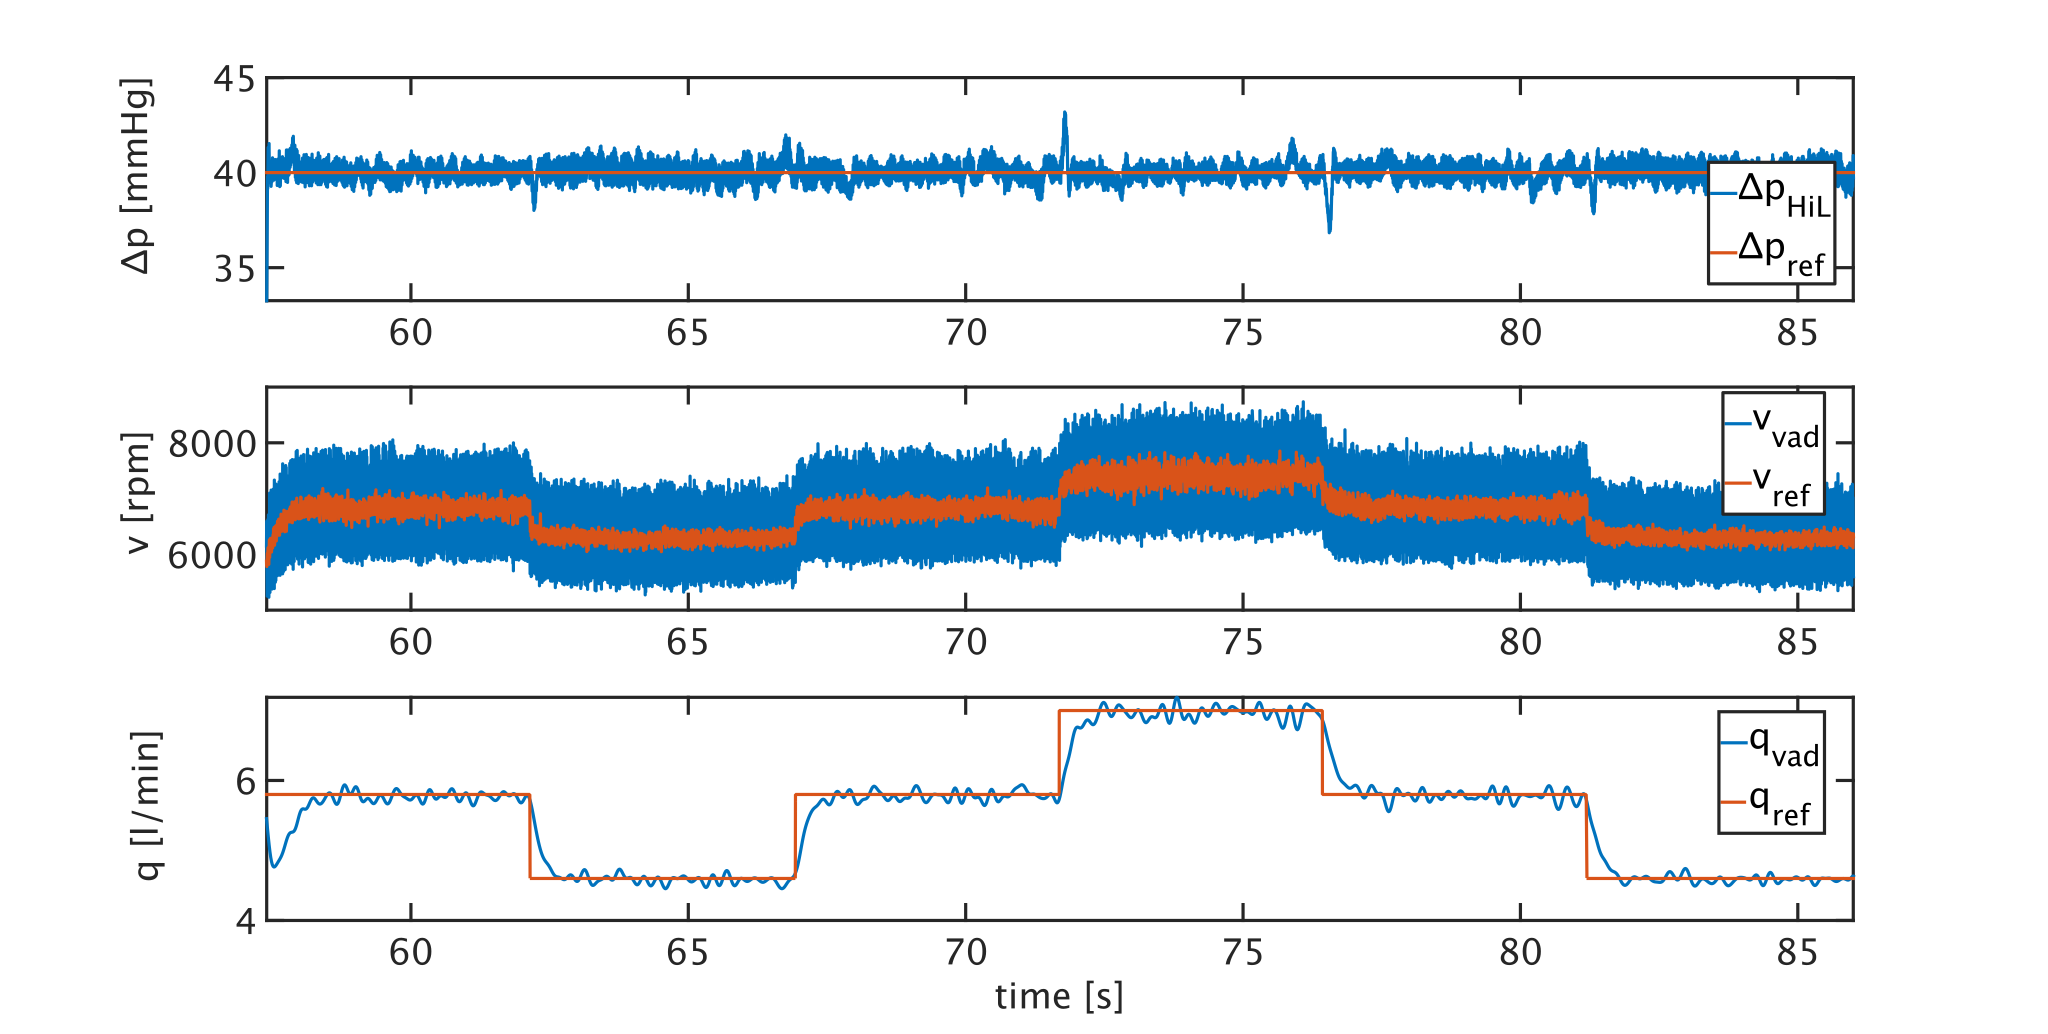
\includegraphics[width=\textwidth]{images/chapt_5/pi_contr_zn_40.pdf}
%   \caption[Step response for determination of PI controller tuning parameters]{Step response for a step in rotational speed of $400\,rpm$ for determination of PI controller tuning parameters.}
%   \label{fig:pi_contr_zn_40}
% \end{figure}

% Dynamische Messung nutzen
% Werte an Sprungstellen
% Nach Wendetangenten verfahren -> GRAFIK
%Berechnung erklären

\section{Iterative Learning Control}
\subsection{Design and Implementation}
Trigger signal aus simulink generiert
\subsection{Evaluation}

\section{Iterative Learning Control with repeating disturbance}
trigger von Störung
\subsection{Design and Implementation}

\subsection{Evaluation}
Q-Filter optimierung f_c vergleich
Test auf verschiedenen Arbeitsbereichen


\section{Iterative Learning Control with varying disturbance length}
trigger von Störung
\subsection{Design and Implementation}
\subsection{Evaluation}
% \section{Evaluation}
% \subsection{PI Controller}
% % gesamt:
% % rms pi total chr = 0.3705
% % rms pi total zn = 0.5396
% % \begin{figure}[ht]
% %   \centering
% %   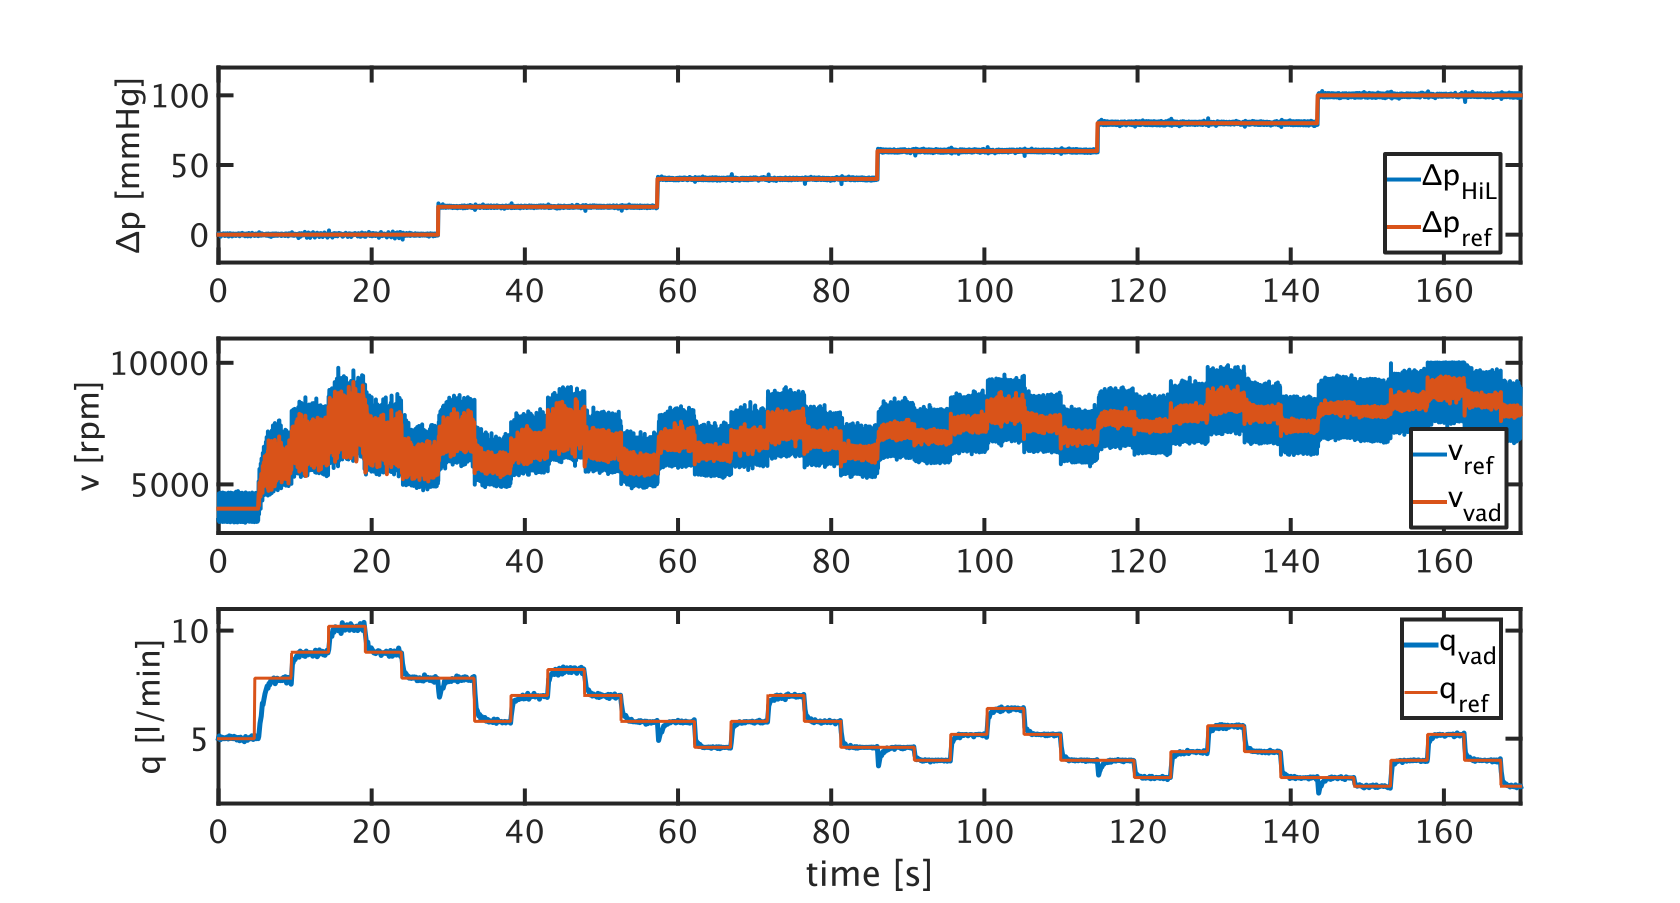
\includegraphics[width=\textwidth]{images/chapt_5/pi_contr_chr.pdf}
% %   \caption[Step response for determination of PI controller tuning parameters]{Step response for a step in rotational speed of $400\,rpm$ for determination of PI controller tuning parameters.}
% %   \label{fig:pi_contr_chr}
% % \end{figure}
%
% % \begin{figure}[ht]
% %   \centering
% %   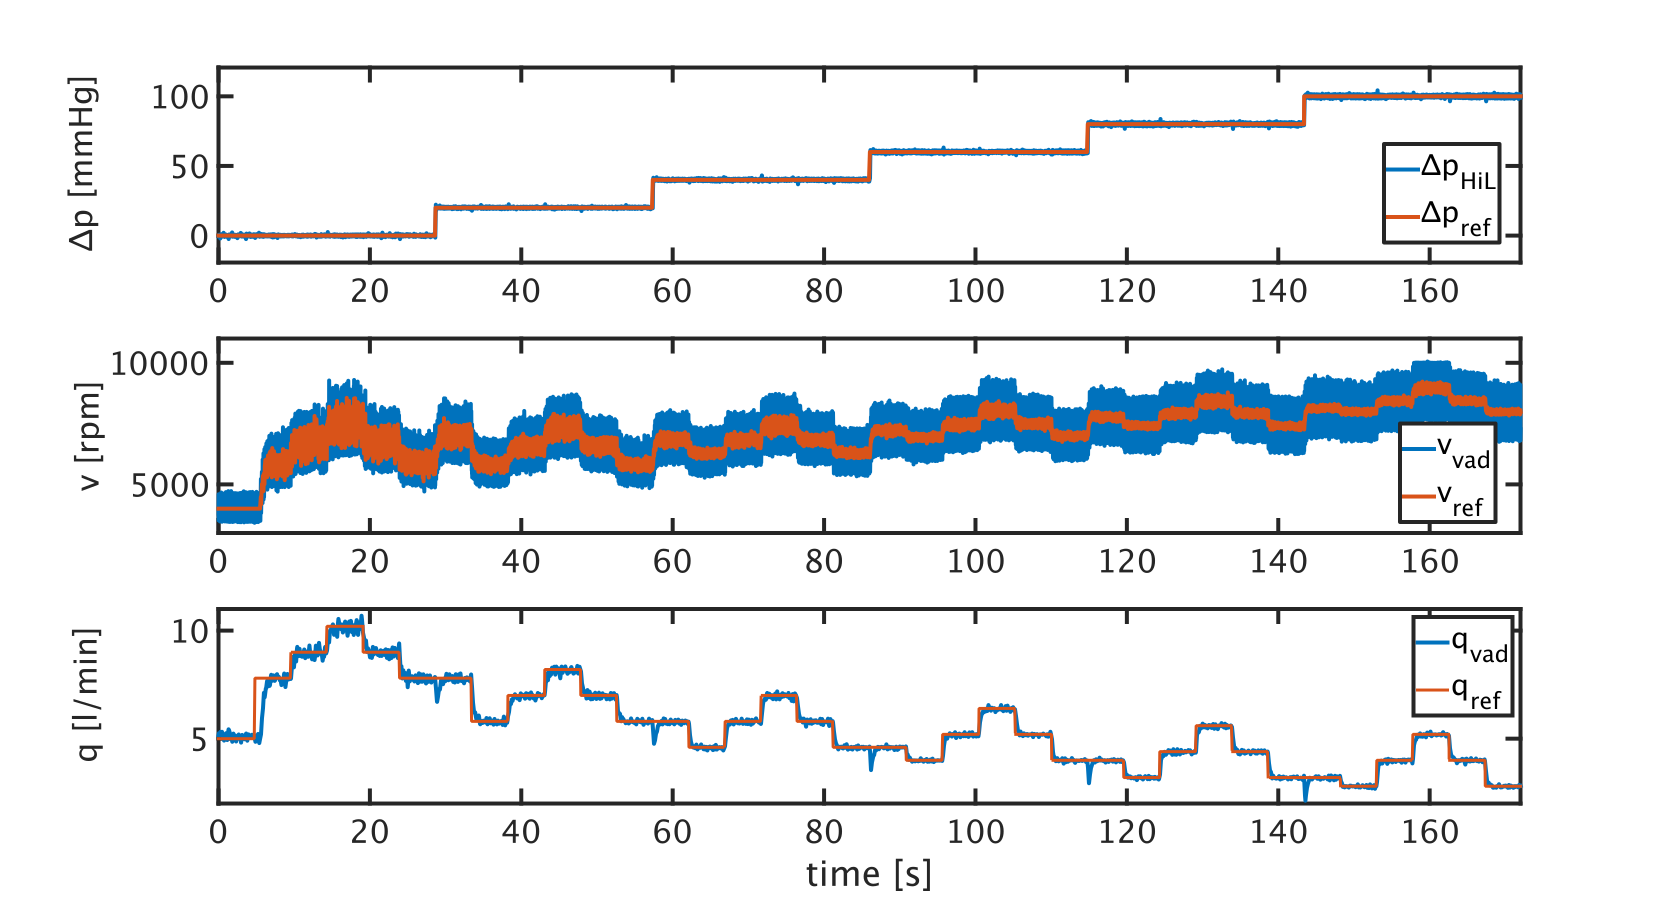
\includegraphics[width=\textwidth]{images/chapt_5/pi_contr_zn.pdf}
% %   \caption[Step response for determination of PI controller tuning parameters]{Step response for a step in rotational speed of $400\,rpm$ for determination of PI controller tuning parameters.}
% %   \label{fig:pi_contr_zn}
% % \end{figure}
%
% % Bereich der Auslegung: 40mmHg
% % RMS PI CHR = 0.2753
% % RMS PI ZN = 0.4013
%
% % \begin{figure}[ht]
% %   \centering
% %   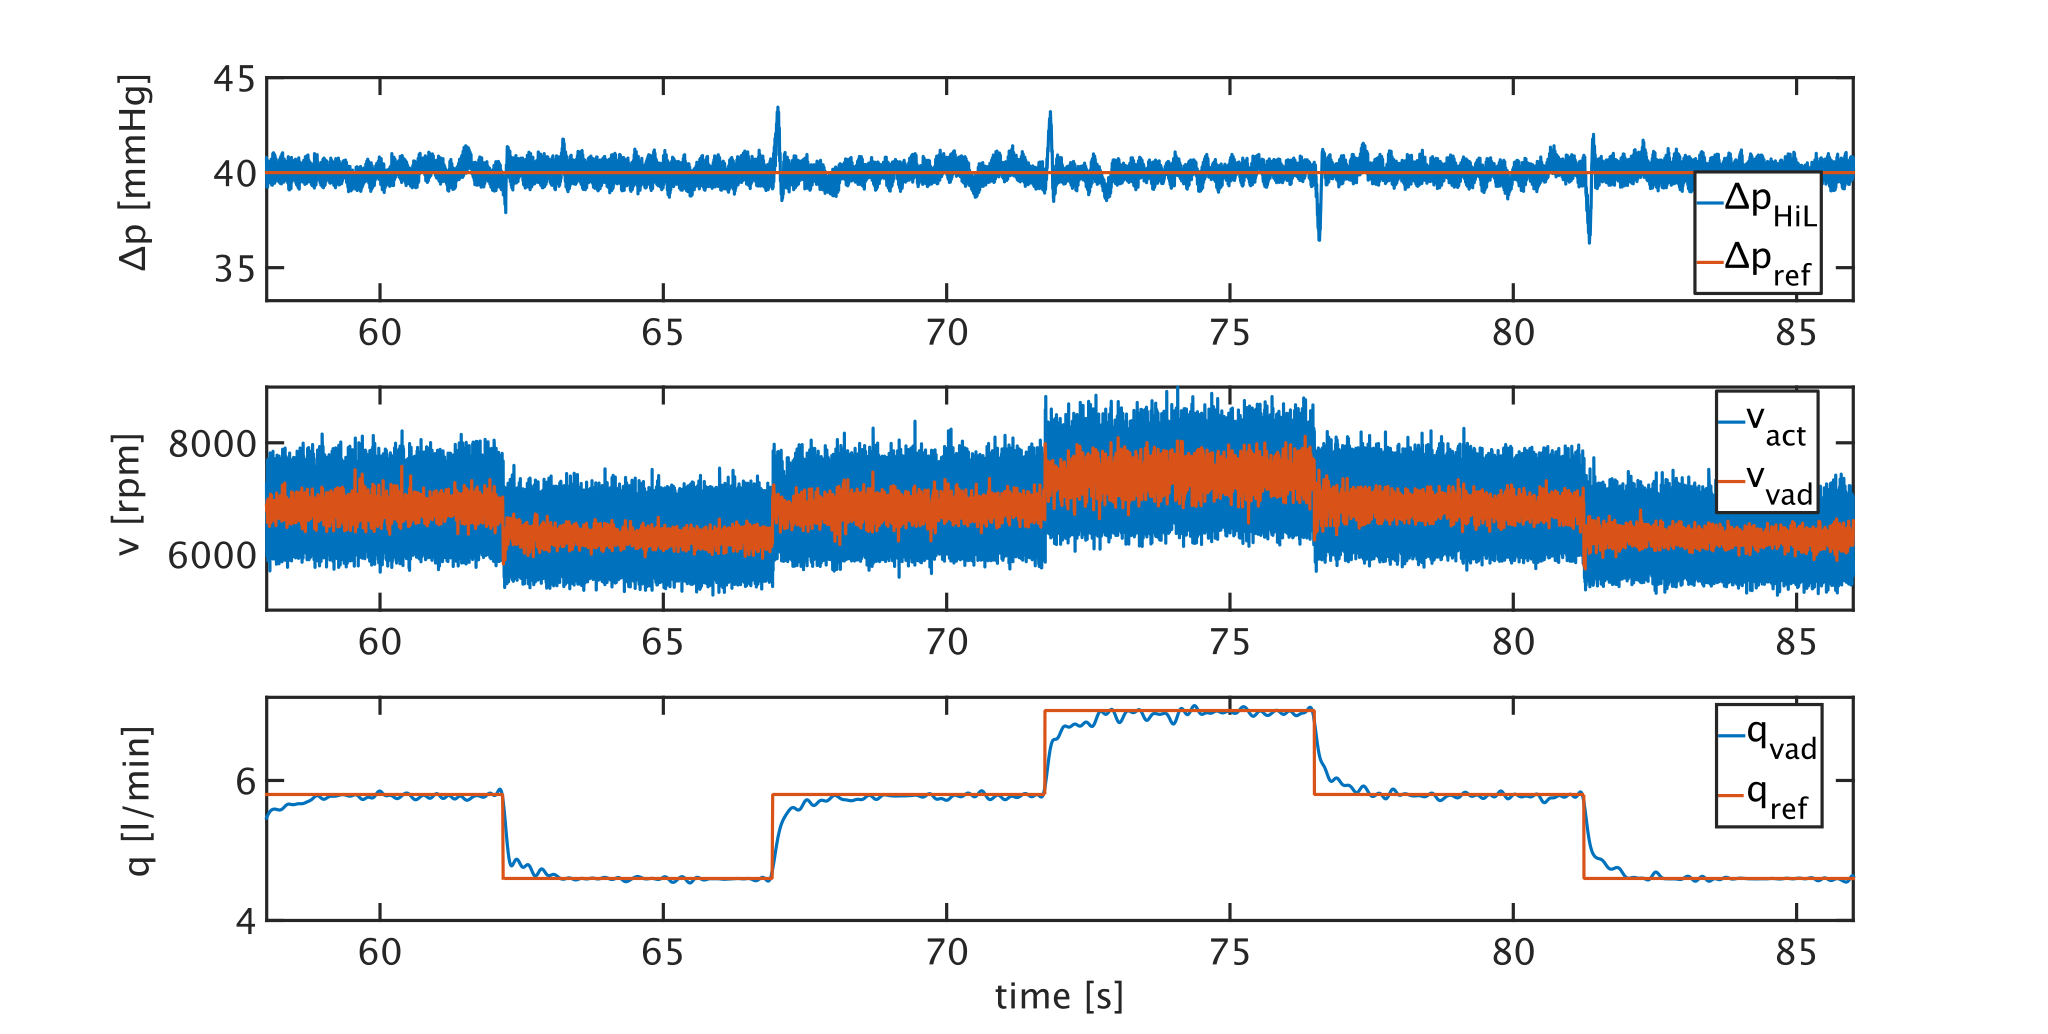
\includegraphics[width=\textwidth]{images/chapt_5/pi_contr_chr_40.pdf}
% %   \caption[Step response for determination of PI controller tuning parameters]{Step response for a step in rotational speed of $400\,rpm$ for determination of PI controller tuning parameters.}
% %   \label{fig:pi_contr_chr_40}
% % \end{figure}
%
% % \begin{figure}[ht]
% %   \centering
% %   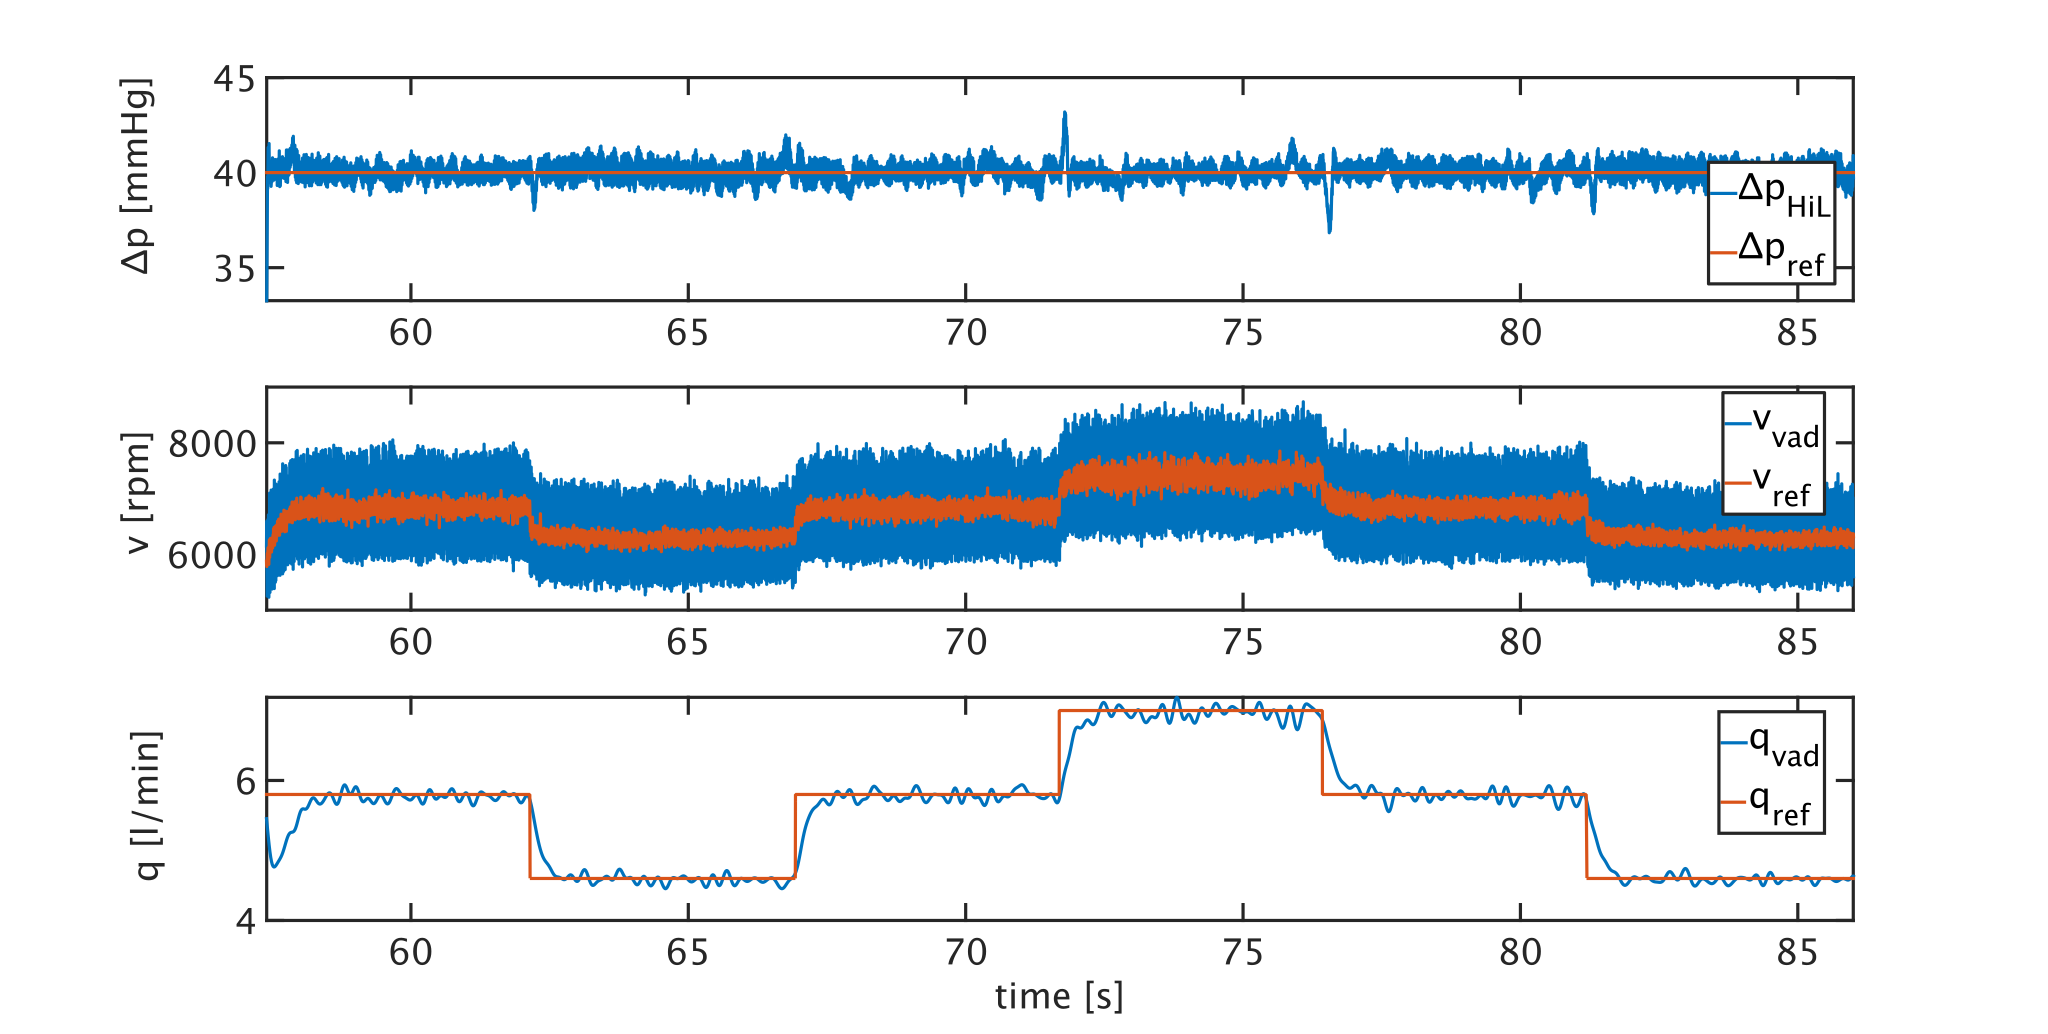
\includegraphics[width=\textwidth]{images/chapt_5/pi_contr_zn_40.pdf}
% %   \caption[Step response for determination of PI controller tuning parameters]{Step response for a step in rotational speed of $400\,rpm$ for determination of PI controller tuning parameters.}
% %   \label{fig:pi_contr_zn_40}
% % \end{figure}
%
% % Dynamische Messung nutzen
% % Werte an Sprungstellen
% % Nach Wendetangenten verfahren -> GRAFIK
% %Berechnung erklären
% \subsection{Iterative Learning Control}
% \subsection{Iterative Learning Control with varying iteration length}
% % Kontanten Fluss über verschiedene Druckbereiche?
% %
% % %Druckverlauf ohne Störung
% %
% % Herzschlag dazu - Druckverlauf

\chapter{Conclusion and future work}
\section{Conclusion}
As the gap between the incidence of cardiovascular disease and the availability of donor organs will continue to grow in the coming years due to demographic change, it is of increasing importance to further develop alternative therapies for CVDs.
For this reason, a flow control system for the Sputnik VAD axial flow pump was developed in the context of this work, enabeling the system to follow different predefined flow trajectories.
\\This was achieved by a stepwise development and optimization of a control loop, which comprises a parallel architecture of a PI controller and an ILC.
\\First, the performance of two PI controllers, designed using the Ziegler Nichols and Chien Hrones Reswick methods, was compared. The second one showed a significantly higher performance, which led to its further use within the ILC implementation as a stabilizing feedback controller.
\\After successful optimization of the Q-filter implemented within the ILC, a series of tests were performed to determine the quality of the ILC. Under the idealized assumption of disturbance by a heartbeat with regular heart rate of $60\, bpm$ and adjustment of the length of the flow trajectories to a duration of $1\,s$ per iteration, satisfactory results were obtained with averaged error values ranging from $RMSE_{\mathrm{rect}}=0.22\,l/min$ for a rectangular trajectory to $RMSE_{\mathrm{sine}}=0.09\,l/min$ for a sinusoidal trajectory. When the standard ILC was subjected to a non-repetitive disturbance in the form of heartbeats of variable heart rates, a significant degradation in performance was evident. For this case, the averaged error values amounted to $RMSE_{\mathrm{rect}}=0.77\,l/min$ for the rectangular signal. For a constant reference flow, it peaked at $RMSE_{\mathrm{const}}=1.13\, l/min$.
\\In order to ensure high performance even in the presence of variable disturbances, the ILC was extended by further data preprocessing in the form of resampling of the ILC's actuating variable data to an iteration length corresponding to the current heart rate. This allowed the averaged error values for a constant flow to be reduced to just $RMSE_{\mathrm{resampled,const}}=0.05\, l/min$. A noticeable improvement in performance was also achieved for a sinusoidal and a triangular signal. Only for the rectangular signal no clear increase in performance could be seen.
For all four reference trajectories tested, however, the pump stopped after some time because the actuating variable exhibited oscillating behavior.

\section{Future work}
In order to ensure long-term flow control under the influence of non-repeating disturbances, as would be necessary for use on patients, the robustness of the controller to this type of disturbance would have to be optimized.

Conceivable approaches to achieve this goal could be given in the use of other ILC implementations, such as a current iteration learning control. Also, the use of a higher-order learning algorithm, which uses not only the last but also even earlier iterations for the calculation, would be recommendable.

One possible hardware improvement with respect to the robustness of the control system would be to use the control unit associated with the Sputnik VAD instead of the ESCON 50/4 EC-S.

For employment of the resampling functionality, as implemented in this work to improve the ILC for non-repetitive disorders, the additional analysis of ECG data would be necessary in clinical use.
\\However, since the Sputnik pump is a therapeutic option with the therapeutic goal of bridging to transplantation, it is conceivable that a patient may require prolonged support from the system. In such a case, it would be desirable not to restrict the patient's mobility and quality of life with an additional medical device. For this reason, a further development of the ILC approach, which would make the use of an ECG signal obsolete, would be desirable.



%**********
%* Anhang *
%**********

\cleardoublepage
\appendix
\chapter{Appendix}
 %\section{System Identification}\label{A1}
\begin{figure}[ht!]
  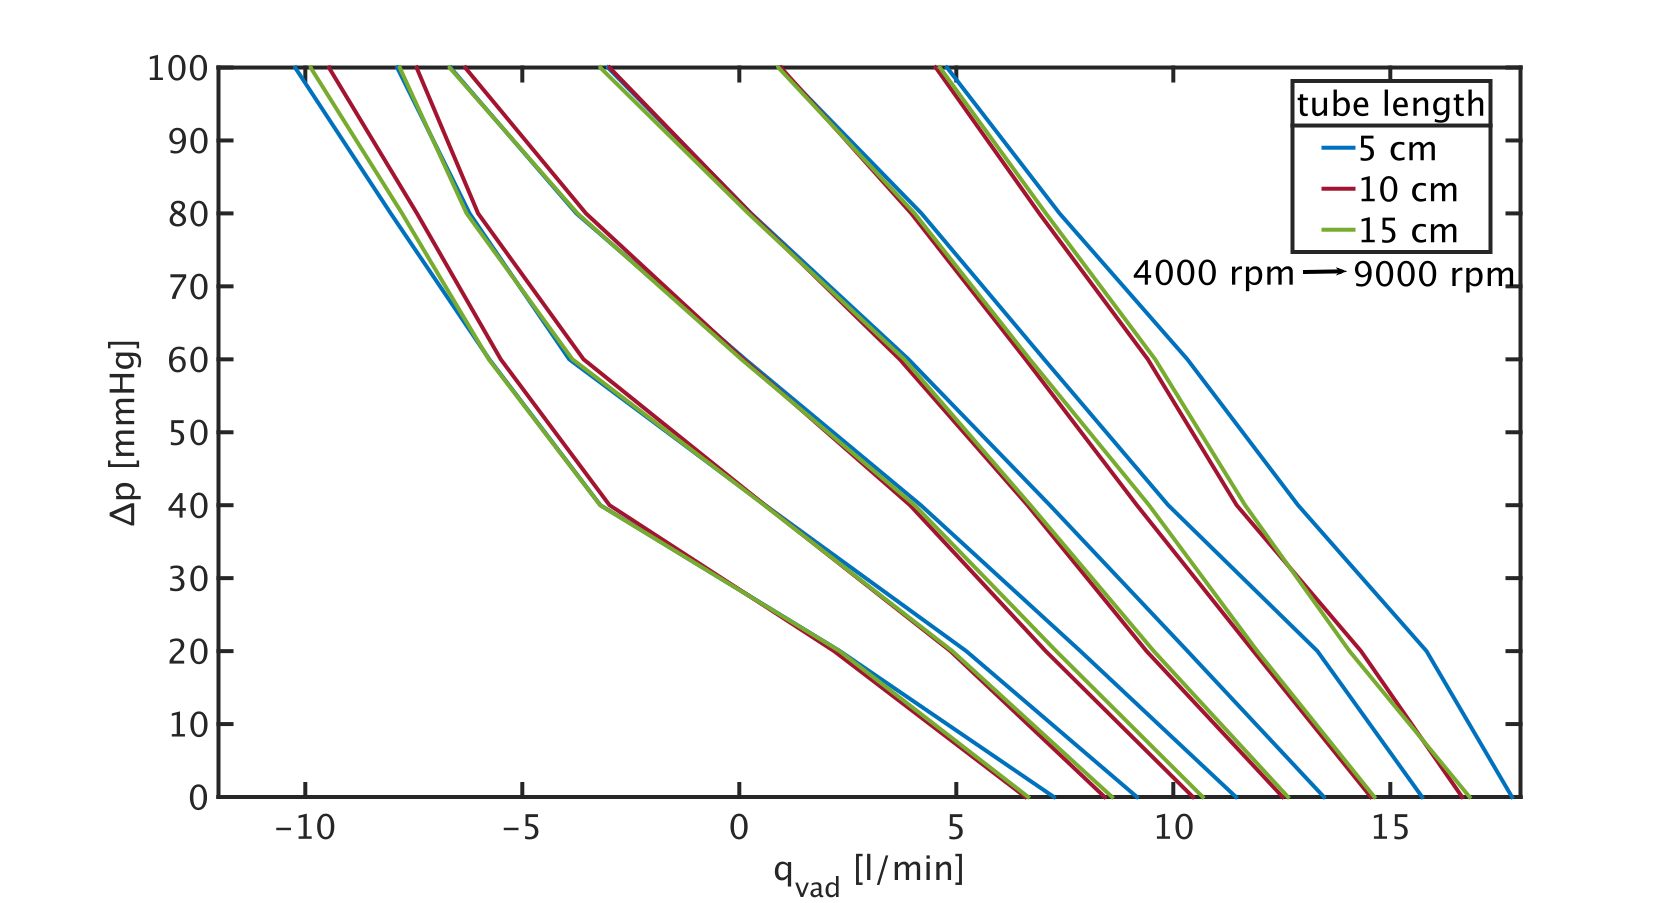
\includegraphics[width=\textwidth]{images/chapt_4/100w_tube_length_new.pdf}
  \caption[Static map for different tube length in 100 \% water]{Static map for varying tube length in 100 \% water}
  \label{fig:anh_1}
\end{figure}

\begin{figure}[ht!]
  \includegraphics[width=\textwidth]{images/chapt_4/80w20g_tube_length_new.pdf}
  \caption[Static map for different tube length in 80 \% water 20 \% glycerin solution]{Static map for varying tube length in 80 \% water 20 \% glycerin solution}
 \label{fig:anh_2}
\end{figure}

\begin{figure}[ht!]
  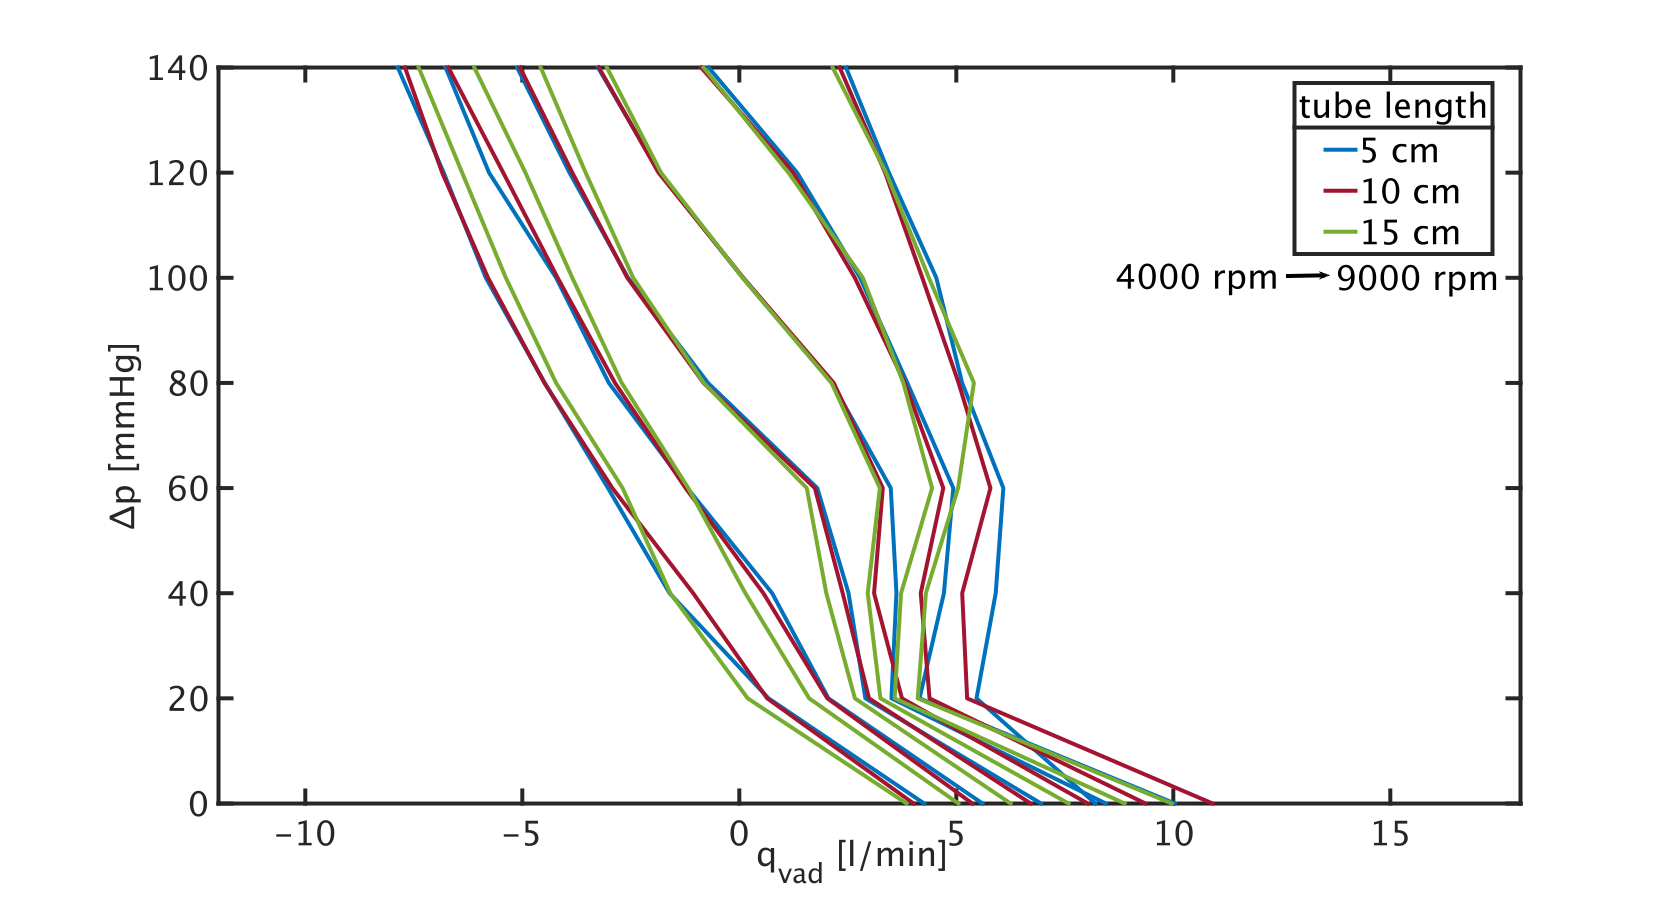
\includegraphics[width=\textwidth]{images/chapt_4/40w60g_tube_length_new.pdf}
  \caption[Static map for different tube length in 40 \% water 60 \% glycerin solution]{Static map for varying tube length in 40 \% water 60 \% glycerin solution}
    \label{fig:anh_3}
\end{figure}

\begin{figure}[ht!]
  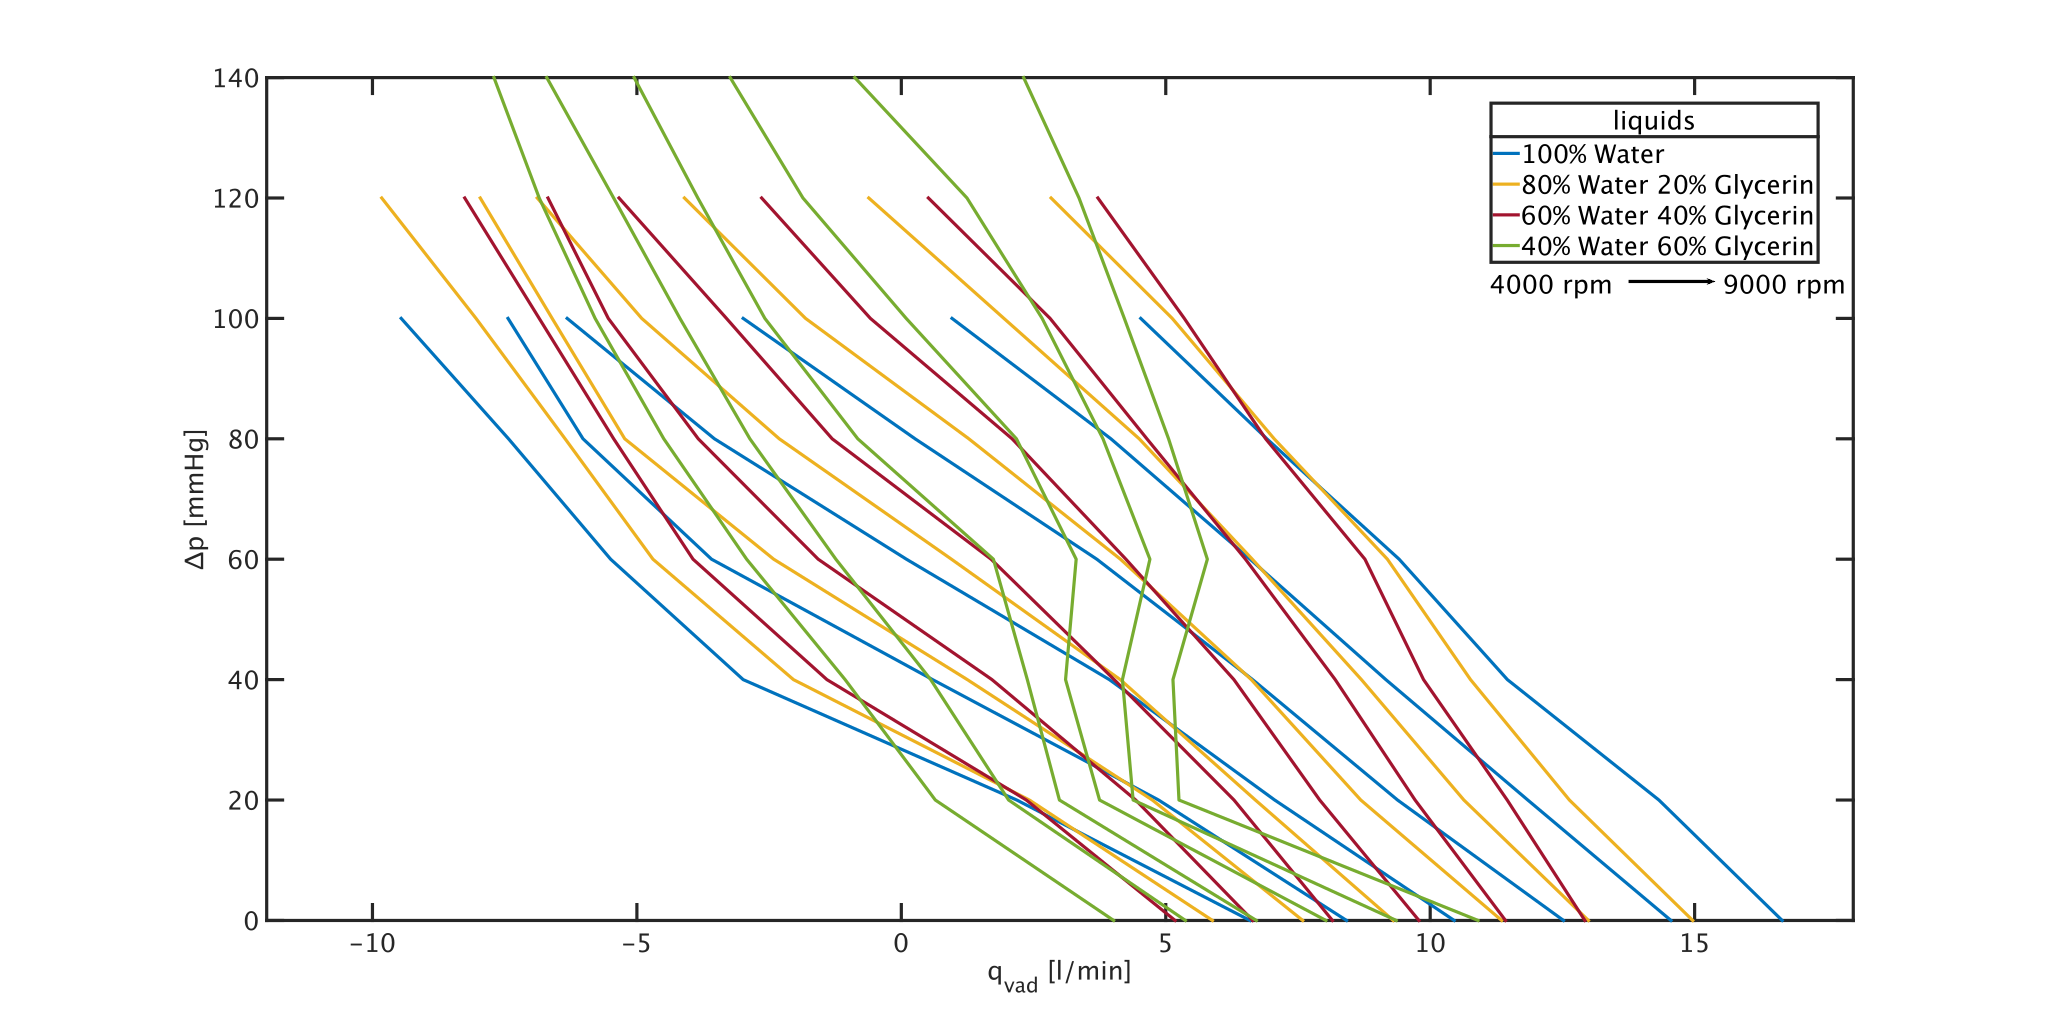
\includegraphics[width=\textwidth]{images/chapt_4/medium_liquid_change_new.pdf}
  \caption[Static map for varying liquid solutions with $10\,cm$ tube length]{Static map for varying liquid solutions with $10\,cm$ tube length.}
    \label{fig:anh_4}
\end{figure}

\begin{figure}[ht!]
  \includegraphics[width=\textwidth]{images/chapt_4/short_liquid_change_new.pdf}
  \caption[Static map for varying liquid solutions with $5\,cm$ tube length]{Static map for varying liquid solutions with $5\,cm$ tube length.}
    \label{fig:anh_5}
\end{figure}

 %\section{Flow Control}
% \subsection{PI Controllers}\label{A2_1}
\begin{figure}[ht!]
  \centering
  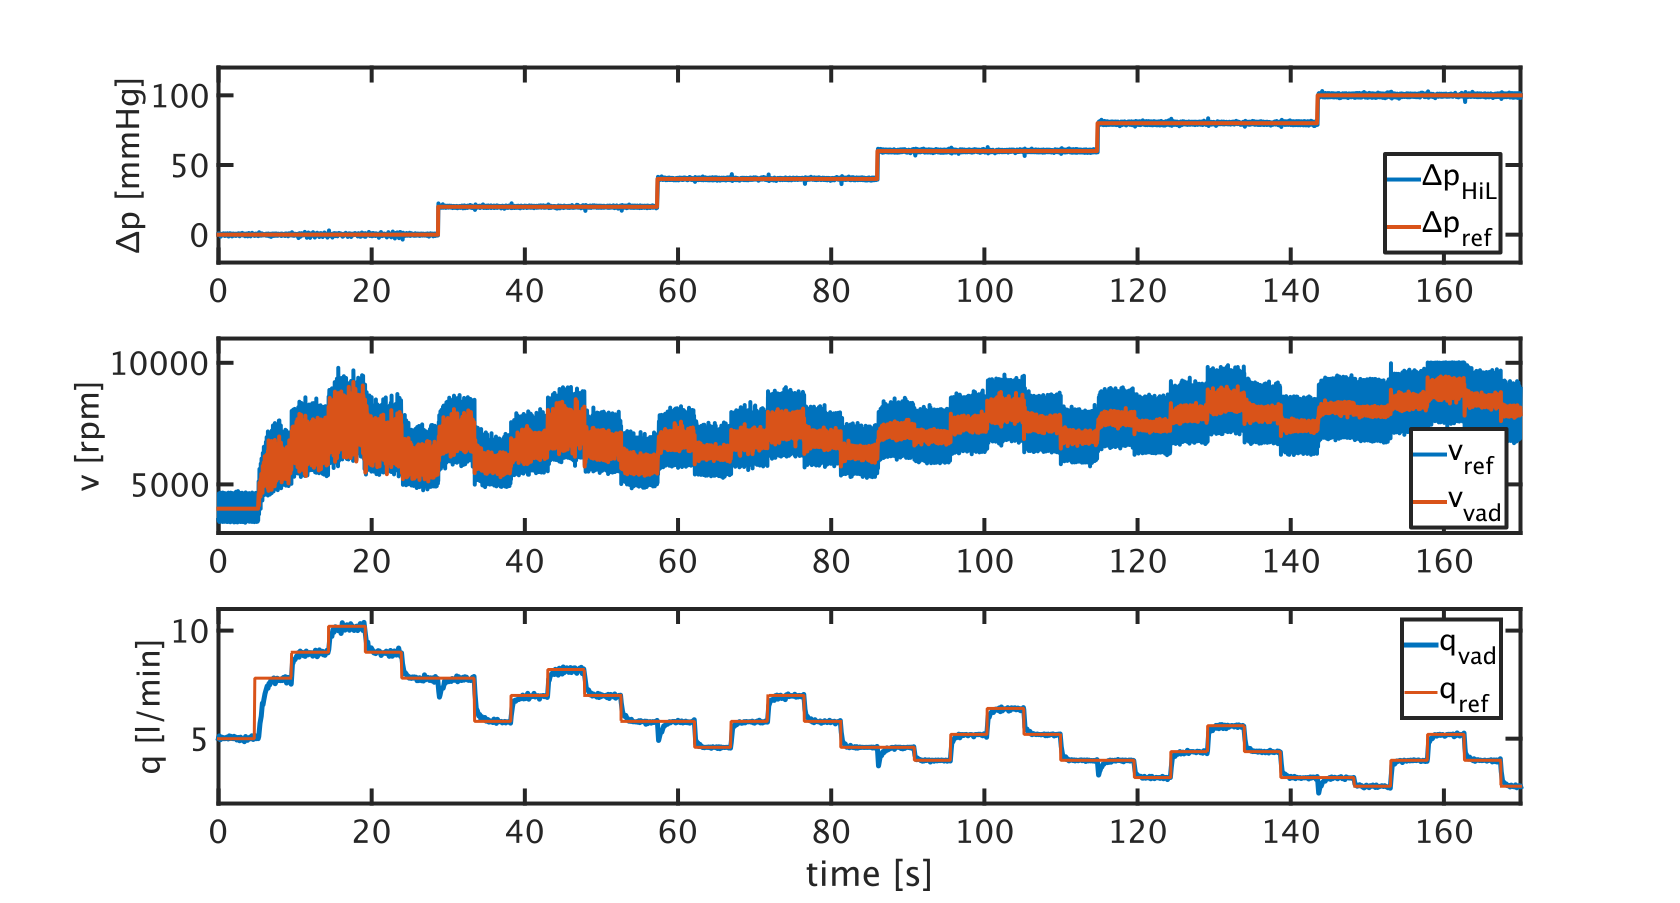
\includegraphics[width=\textwidth]{images/chapt_5/pi_contr_chr.pdf}
  \caption[Test measurement for PI controller tuned according to Chien Hrones Reswick]{Test measurement for PI controller tuned according to Chien Hrones Reswick.}
  \label{fig:anh_6}
\end{figure}

\begin{figure}[ht!]
  \centering
  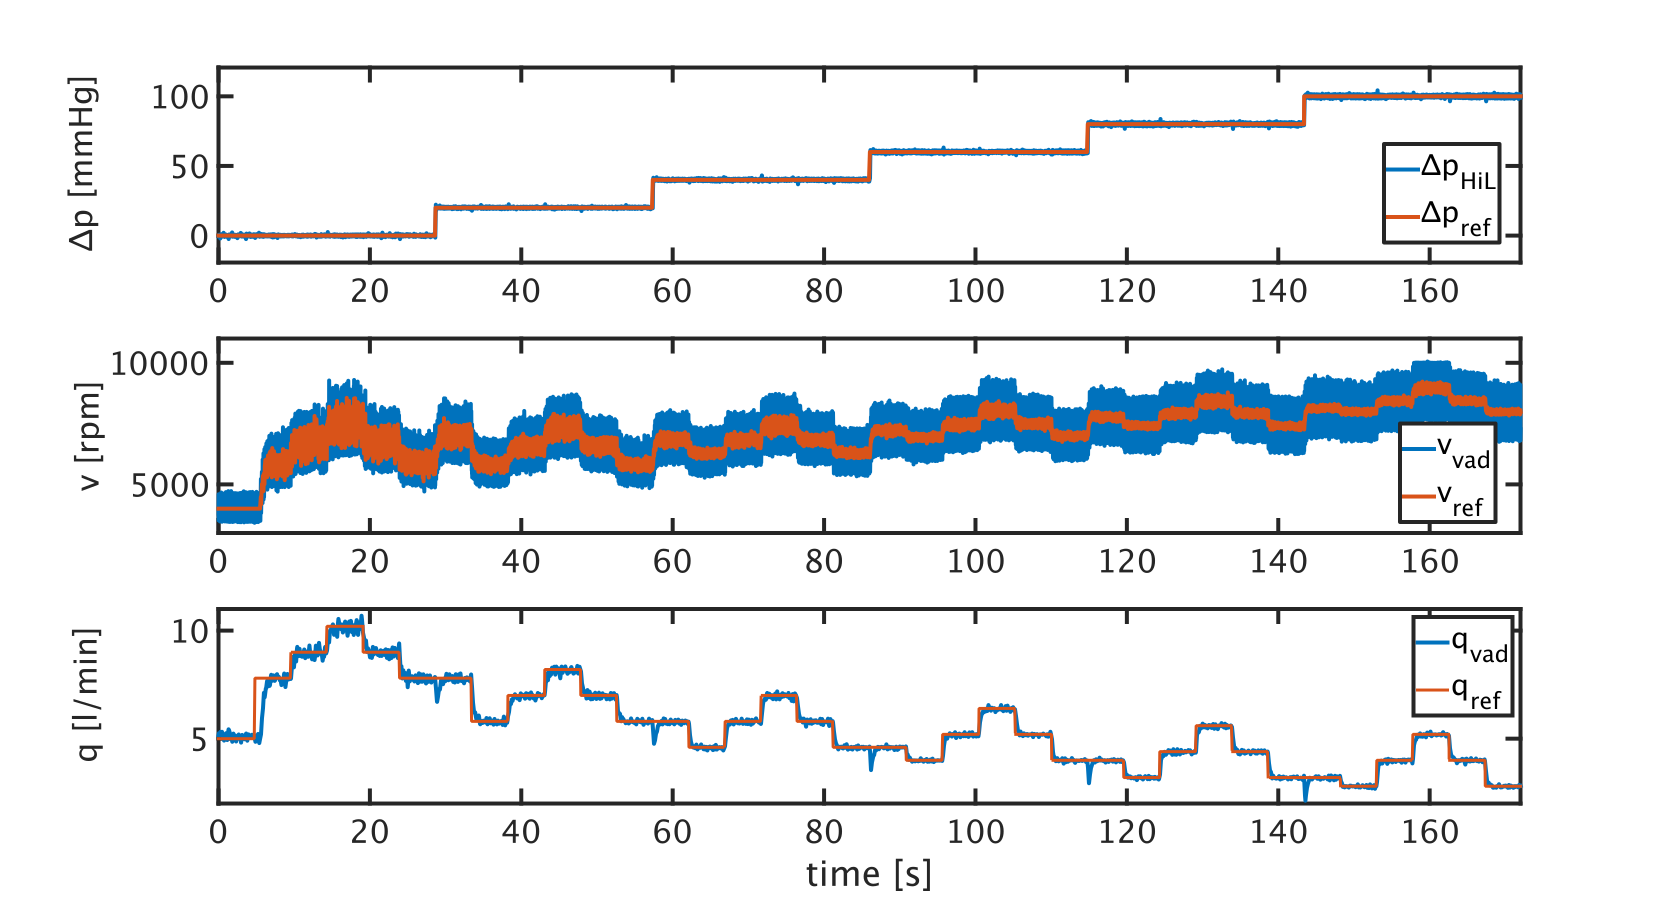
\includegraphics[width=\textwidth]{images/chapt_5/pi_contr_zn.pdf}
  \caption[Test measurement for PI controller tuned according to Ziegler Nichols]{Test measurement for PI controller tuned according to Ziegler Nichols.}
  \label{fig:anh_7}
\end{figure}

\begin{figure}[ht!]
  \centering
  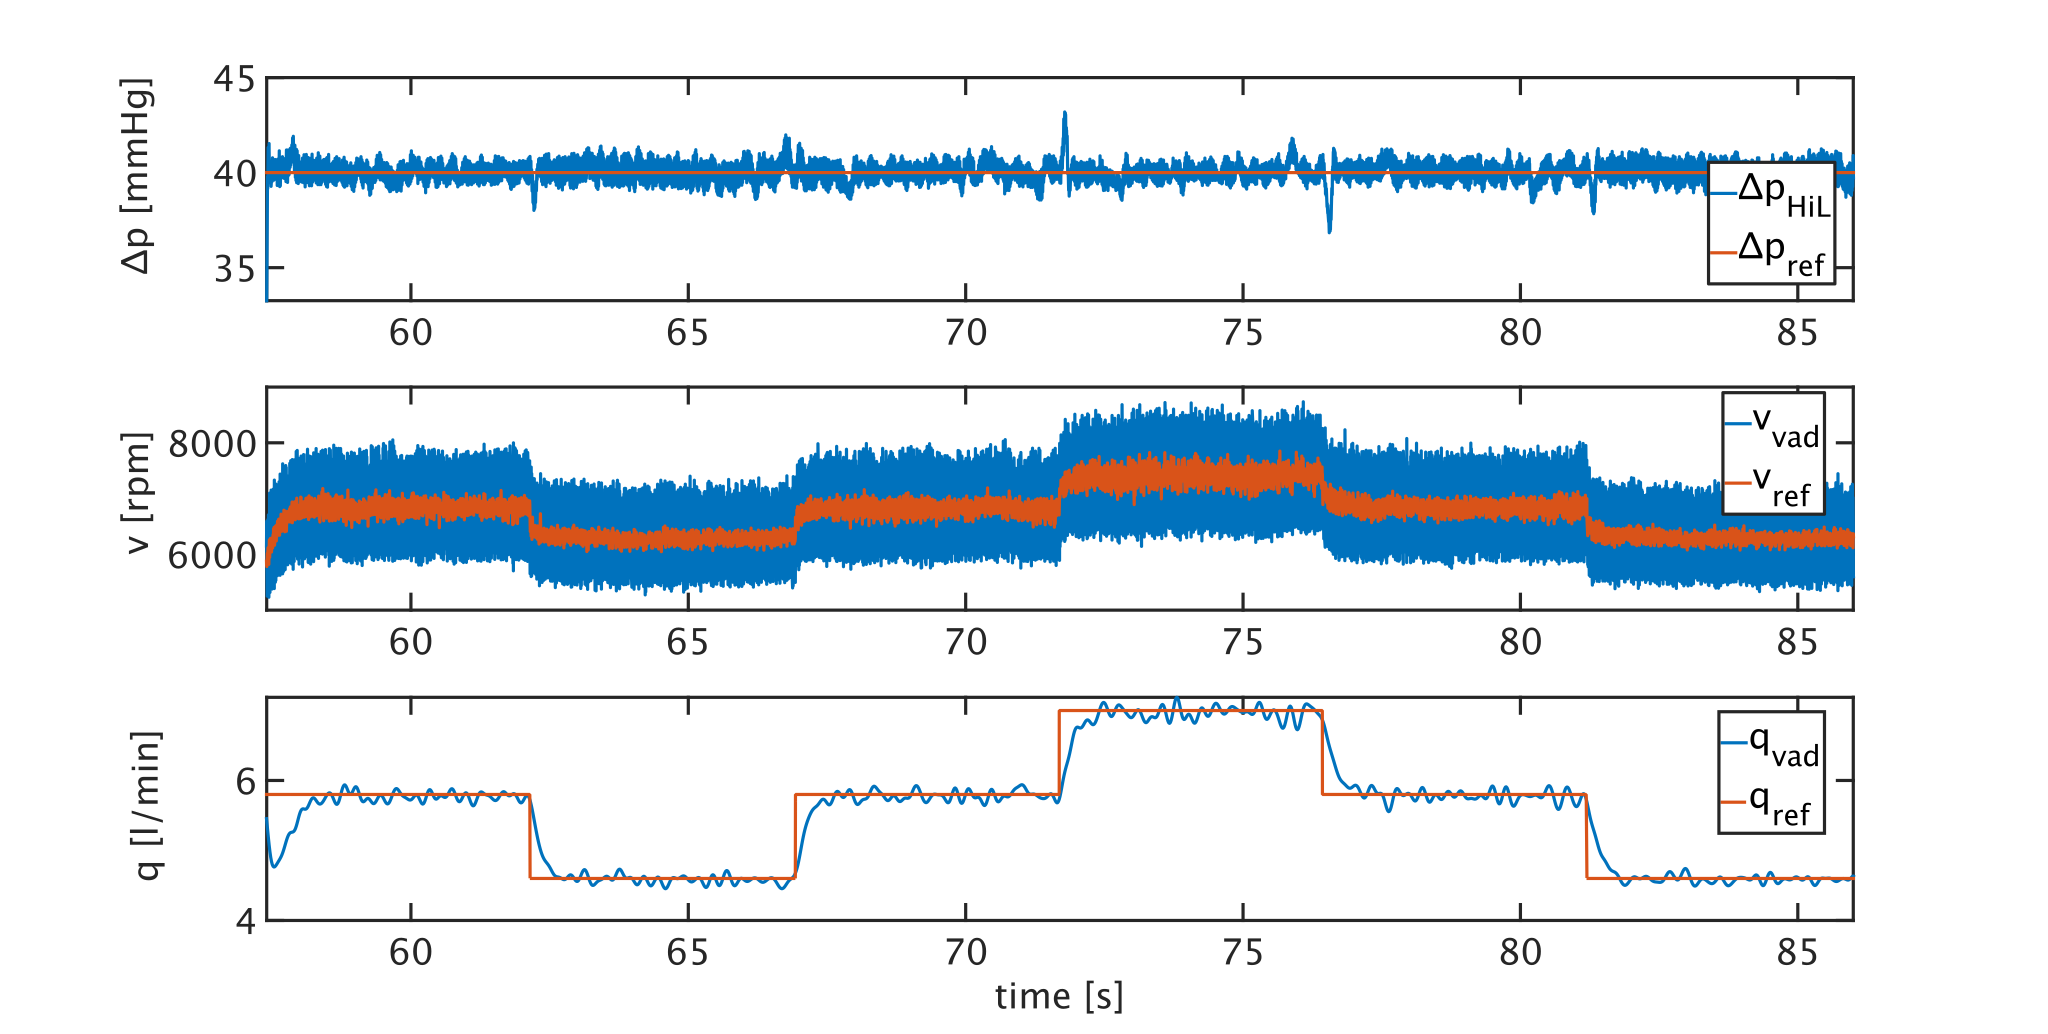
\includegraphics[width=\textwidth]{images/chapt_5/pi_contr_zn_40.pdf}
  \caption[Test measurement for PI controller tuned according to Ziegler Nichols at $\Delta{p}=40\,mmHg$]{Test measurement for PI controller tuned according to Ziegler Nichols at $\Delta{p}=40\,mmHg$.}
  \label{fig:anh_8}
\end{figure}

%\section{ILC with varying disturbance}

\begin{figure}[ht!]
  \centering
  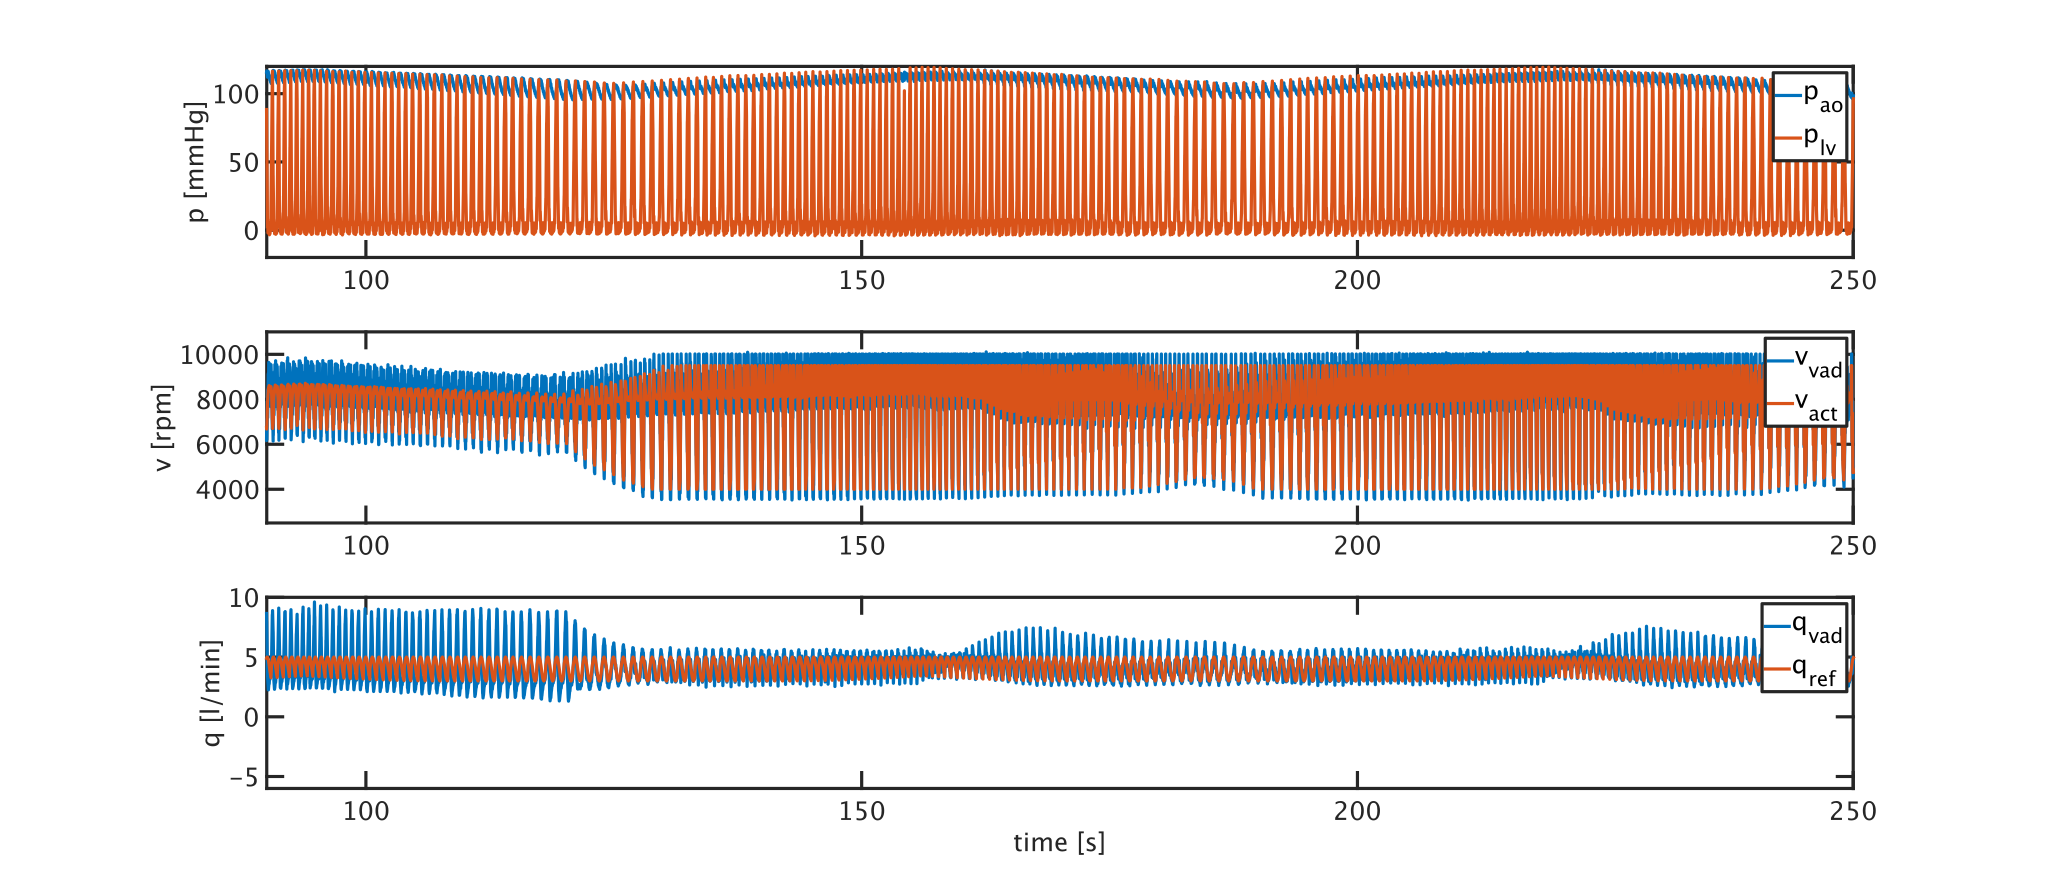
\includegraphics[width=0.95\textwidth]{images/chapt_5/ILC/ilc_var_dist_unfix_sine.pdf}
  \caption[Segment of measurement for ILC with varying disturbance with $cf_{\mathrm{Lv}}=1$ for sinusoidal reference flow without data resampling]{Segment of measurement for ILC with varying disturbance with $cf_{\mathrm{Lv}}=1$ for sinusoidal reference flow without data resampling. Top:  pressure values of the MCL. Middle: actuating variable and measured rotational speed of the VAD. Bottom: targeted flow trajectory and measured flow through the VAD}
 % \label{fig:ilc_var_dist_unfix_sine}
 \label{fig:anh_9}
\end{figure}

\begin{figure}[ht!]
  \centering
  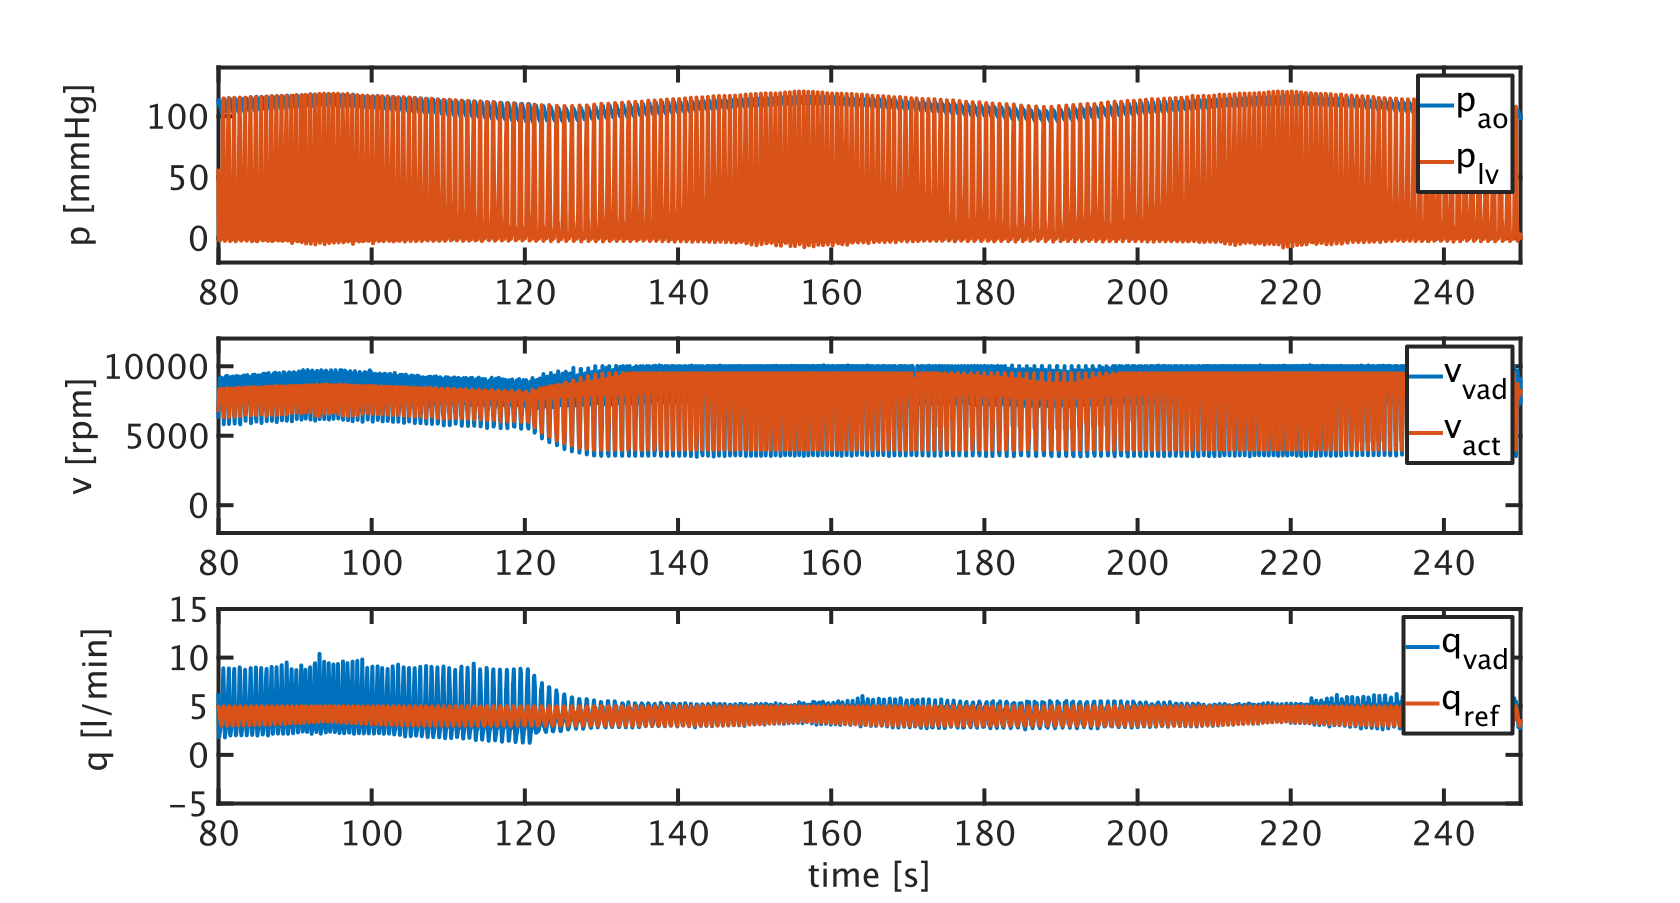
\includegraphics[width=0.95\textwidth]{images/chapt_5/ILC/ilc_var_dist_fix_sine.pdf}
  \caption[Segment of measurement for ILC with varying disturbance with $cf_{\mathrm{Lv}}=1$ for sinusoidal reference flow with data resampling]{Segment of measurement for ILC with varying disturbance with $cf_{\mathrm{Lv}}=1$ for sinusoidal reference flow with data resampling. Top:  pressure values of the MCL. Middle: actuating variable and measured rotational speed of the VAD. Bottom: targeted flow trajectory and measured flow through the VAD}
  %\label{fig:ilc_var_dist_fix_sine}
   \label{fig:anh_10}
\end{figure}

\begin{figure}[ht!]
  \centering
  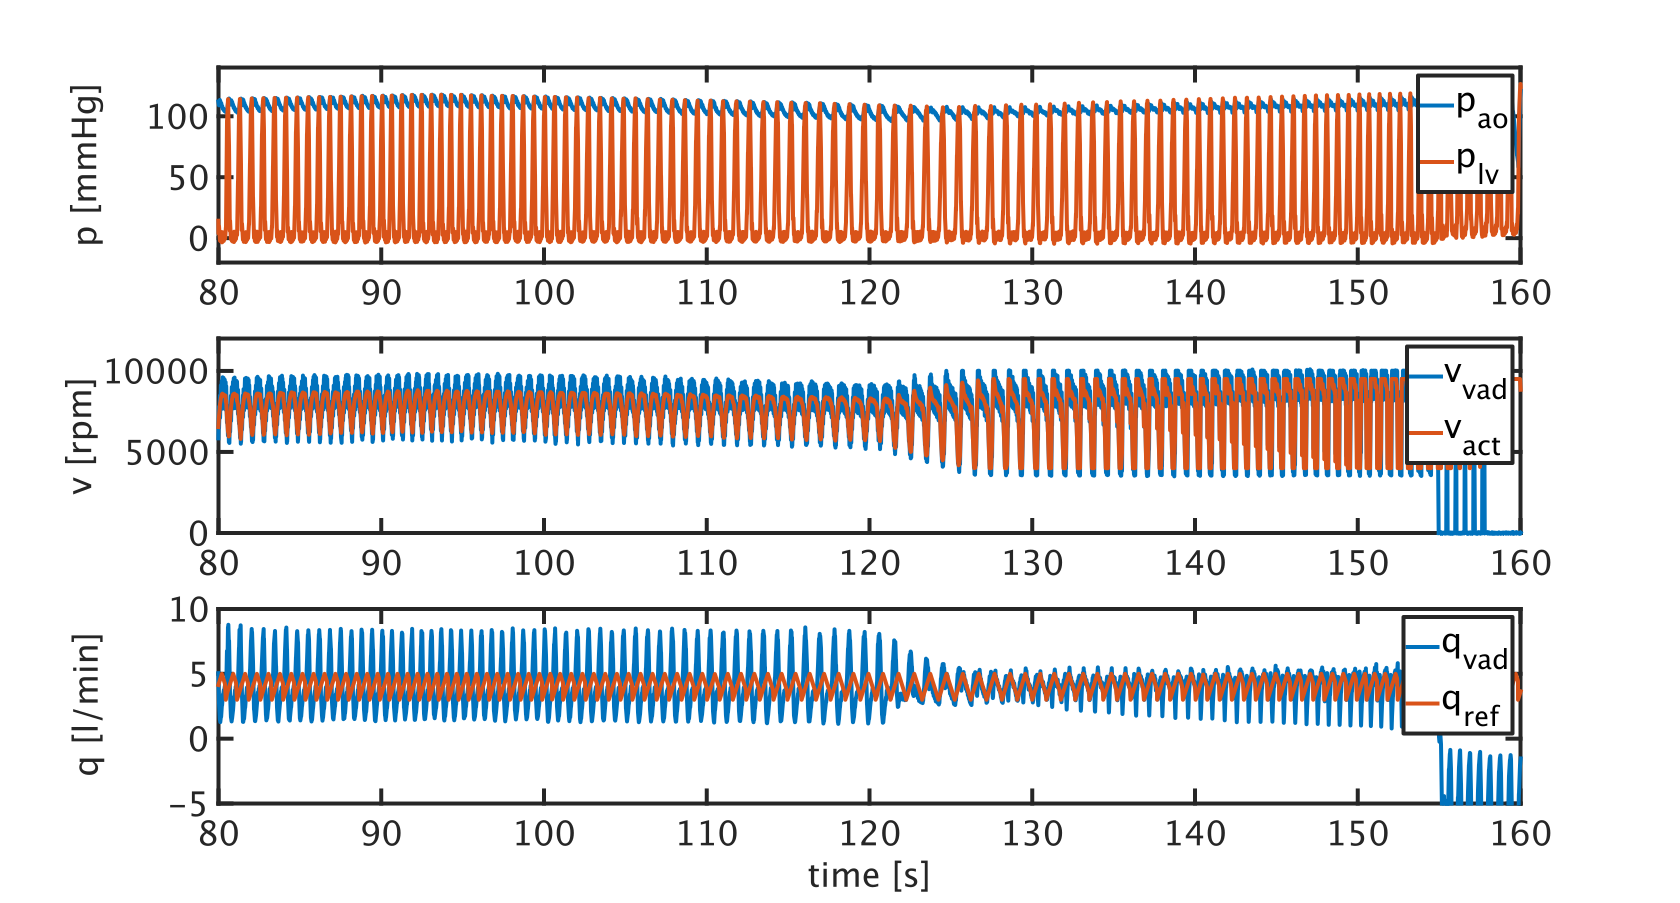
\includegraphics[width=0.95\textwidth]{images/chapt_5/ILC/ilc_var_dist_unfix_triang.pdf}
  \caption[Segment of measurement for ILC with varying disturbance with $cf_{\mathrm{Lv}}=1$ for triangular reference flow without data resampling]{Segment of measurement for ILC with varying disturbance with $cf_{\mathrm{Lv}}=1$ for triangular reference flow without data resampling. Top:  pressure values of the MCL. Middle: actuating variable and measured rotational speed of the VAD. Bottom: targeted flow trajectory and measured flow through the VAD}
  %\label{fig:ilc_var_dist_unfix_triang}
   \label{fig:anh_11}
\end{figure}

\begin{figure}[ht!]
  \centering
  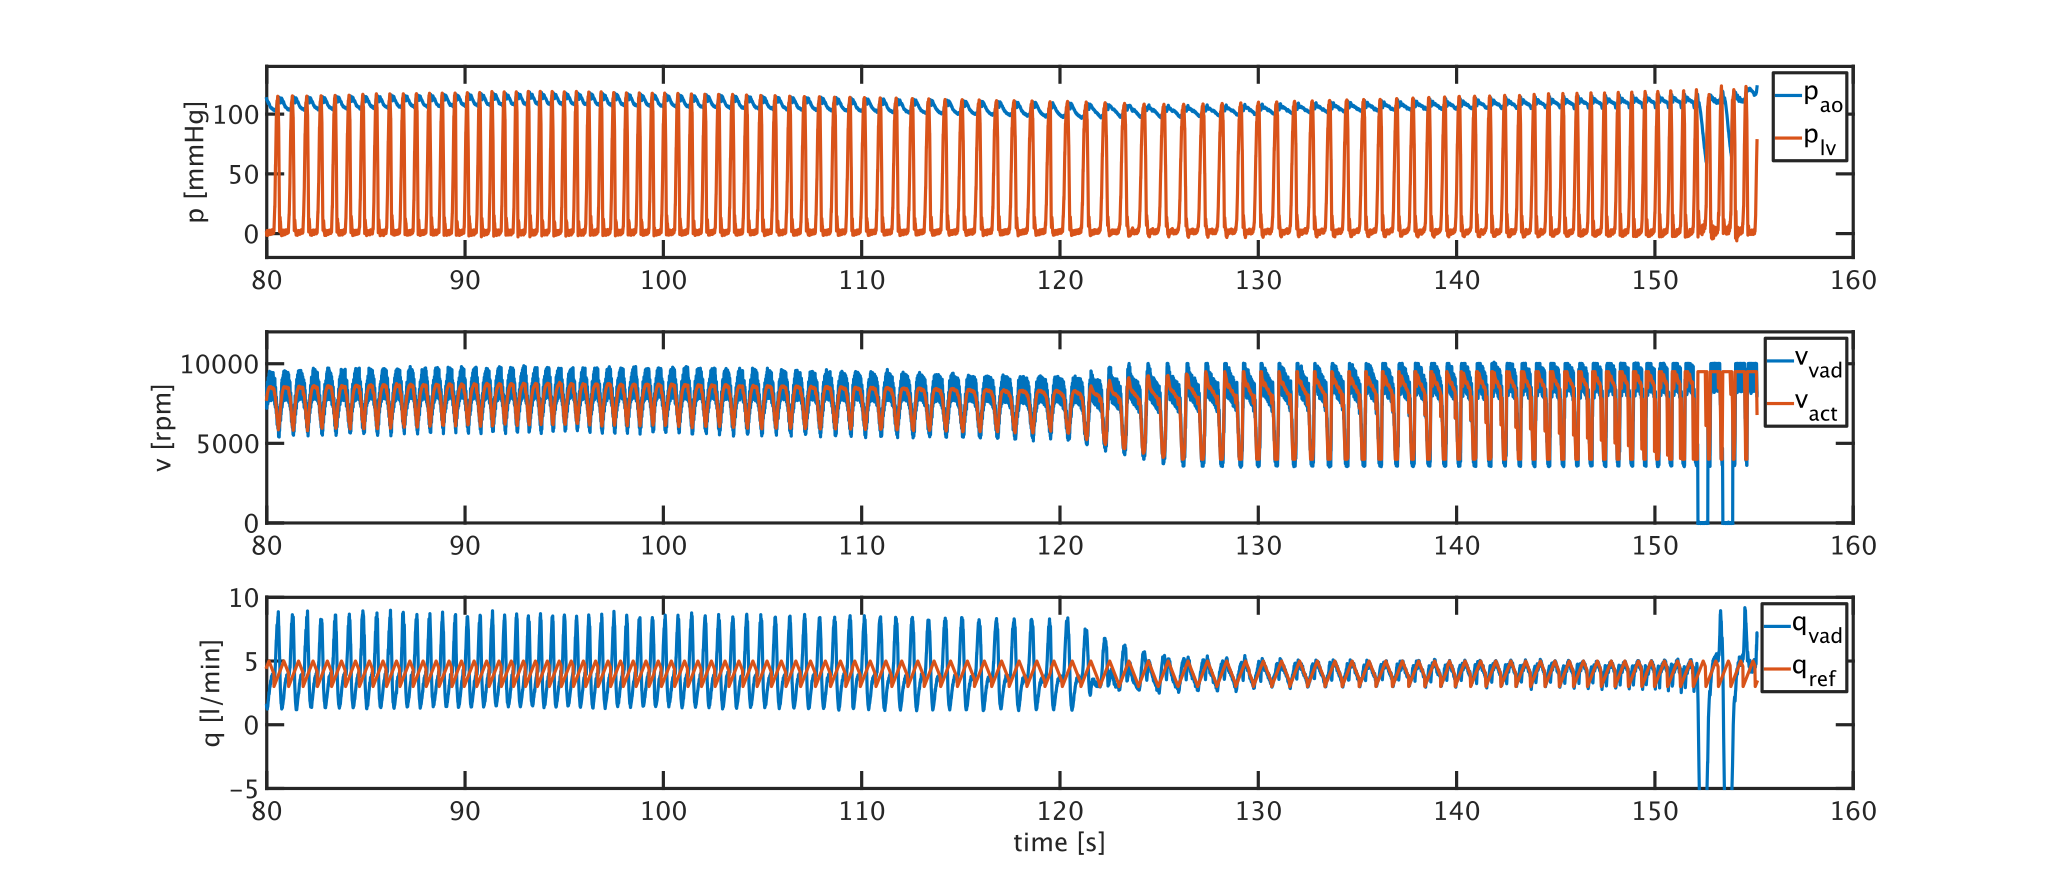
\includegraphics[width=0.95\textwidth]{images/chapt_5/ILC/ilc_var_dist_fix_triang.pdf}
  \caption[Segment of measurement for ILC with varying disturbance with $cf_{\mathrm{Lv}}=1$ for triangular reference flow with data resampling]{Segment of measurement for ILC with varying disturbance with $cf_{\mathrm{Lv}}=1$ for triangular reference flow with data resampling. Top:  pressure values of the MCL. Middle: actuating variable and measured rotational speed of the VAD. Bottom: targeted flow trajectory and measured flow through the VAD}
  %\label{fig:ilc_var_dist_fix_triang}
   \label{fig:anh_12}
\end{figure}

\begin{figure}[ht!]
  \centering
  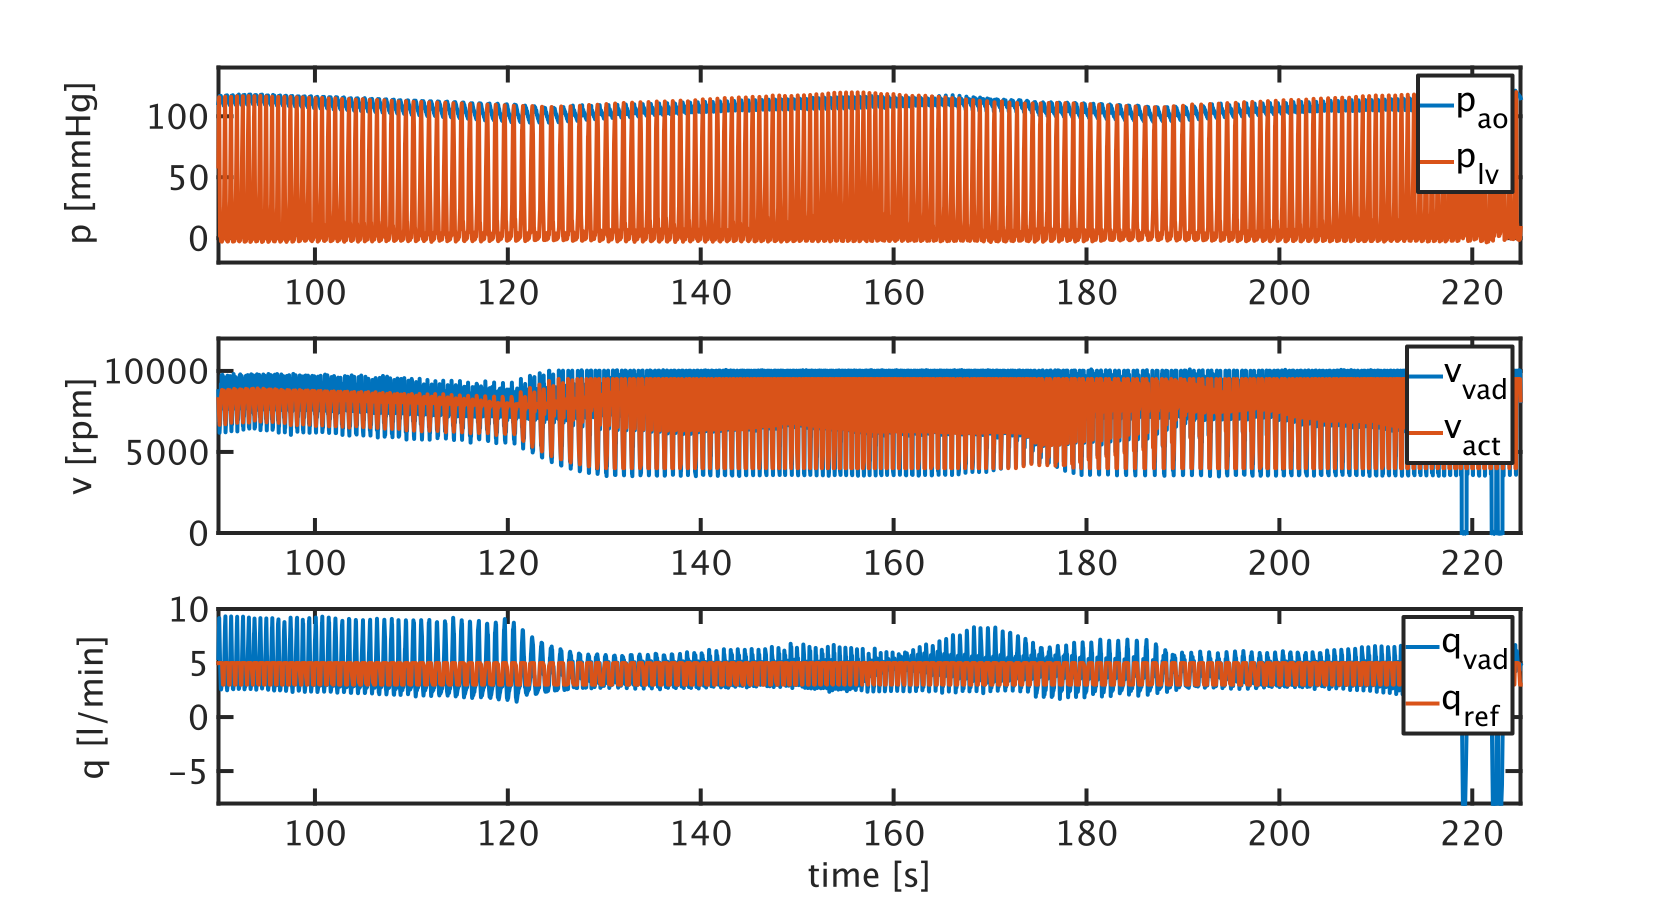
\includegraphics[width=0.95\textwidth]{images/chapt_5/ILC/ilc_var_dist_unfix_rect.pdf}
  \caption[Segment of measurement for ILC with varying disturbance with $cf_{\mathrm{Lv}}=1$ for rectangular reference flow without data resampling]{Segment of measurement for ILC with varying disturbance with $cf_{\mathrm{Lv}}=1$ for rectangular reference flow without data resampling. Top:  pressure values of the MCL. Middle: actuating variable and measured rotational speed of the VAD. Bottom: targeted flow trajectory and measured flow through the VAD}
  %\label{fig:ilc_var_dist_unfix_rect}
   \label{fig:anh_13}
\end{figure}

\begin{figure}[ht!]
  \centering
  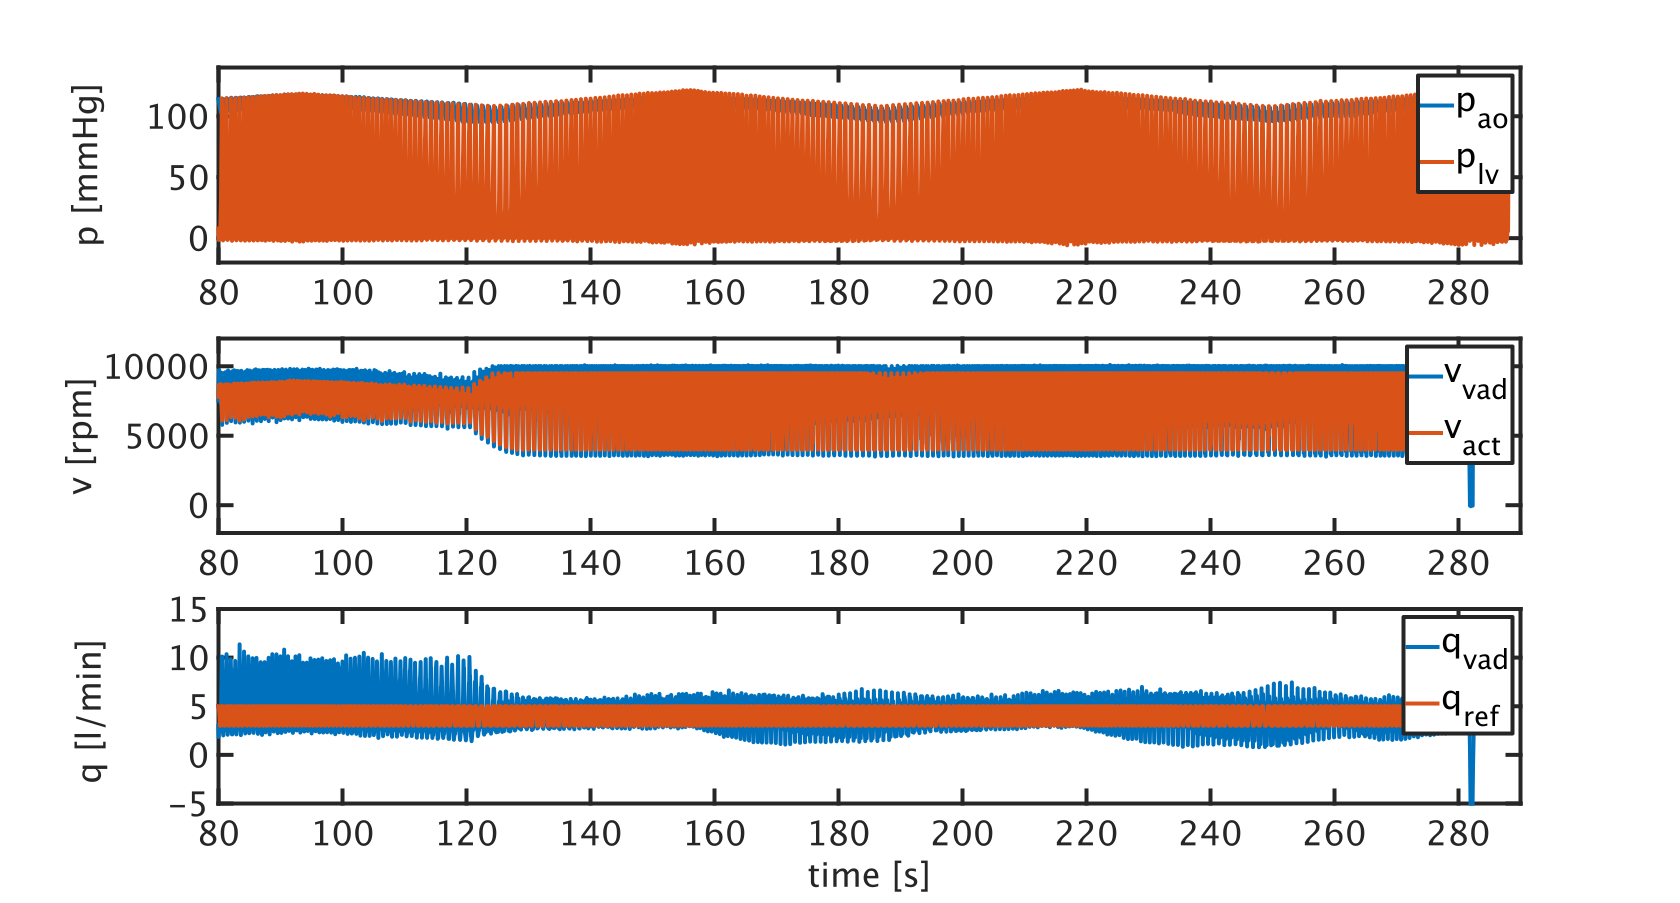
\includegraphics[width=0.95\textwidth]{images/chapt_5/ILC/ilc_var_dist_fix_rect.pdf}
  \caption[Segment of measurement for ILC with varying disturbance with $cf_{\mathrm{Lv}}=1$ for rectangular reference flow with data resampling]{Segment of measurement for ILC with varying disturbance with $cf_{\mathrm{Lv}}=1$ for rectangular reference flow with data resampling. Top:  pressure values of the MCL. Middle: actuating variable and measured rotational speed of the VAD. Bottom: targeted flow trajectory and measured flow through the VAD}
  %\label{fig:ilc_var_dist_fix_rect}
   \label{fig:anh_14}
\end{figure}



%**********************************************************
% Literaturverzeichnis (hier muss nichts ge�ndert werden) *
%**********************************************************

\bibliographystyle{alphadin}    %\bibliographystyle{} plain dinat
\bibliography{literatur}%


\end{sloppypar}
\end{document}
